\documentclass{xdupgthesis}
% \usepackage[backend=bibtex]{biblatex}
\usepackage[backend=biber, style=gb7714-2015]{biblatex}
\usepackage{amsmath}
\usepackage{amssymb}
\usepackage[noend]{algpseudocode}
\usepackage{algorithmicx,algorithm}
\usepackage{float}
\usepackage{subfig}
\usepackage{overpic}
\usepackage{booktabs}
\usepackage{threeparttable}
\usepackage{multirow}
\usepackage{multicol}
\usepackage{diagbox}
\usepackage{graphicx}
\usepackage{longtable}
\usepackage{color}

\xdusetup{
    style = {
        cjk-font = win,
        latin-font = tac,
        % anonymous = true, %盲审 - true
        % remove-header = true  %去掉页眉(没什么用)
        % remove-page = {封面, 提名页, 声明页, 索引, 目录, 附录, 参考文献, 致谢, 作者简介} %查重用
    },
    info = {
        bib-resource = {reference.bib},
        abstract = {abstract_ch.tex}, % 中文摘要
        abstract* = {abstract_en.tex}, % 英文摘要
        los = {los.tex}, % 符号对照表
        loa = {loa.tex}, % 缩略语对照表
        bio = {author.tex}, % 作者简介
        acknowledgements = {acknowledgements.tex}, % 致谢
        title = {分布式深度学习的梯度压缩方法研究及其应用},
        title* = {Research on Gradient Compression Method for Distributed Deep Learning and Its Application},
        author = {\anon[XXX]{卢天恩}}, %盲审用
        author* = {\anon[XXX]{Lu TianEn}}, %盲审用
        department = {通信工程学院},
        graduate-type = {硕士},
        degree-type = {学术},
        degree = {工学硕士},
        major = {信息与通信工程},
        major* = {Information and Communications Engineering},
        sub-major = {多媒体信息理论},
        supervisor = {谢卫莹},
        supervisor* = {Xie WeiYing},
        supervisor-title = {教授},
        supervisor-title* = {Professor},
        % supervisor = {XXX},  %盲审用
        % supervisor* = {XXX}, %盲审用
        % supervisor-title = { }, %盲审用
        % supervisor-title* = { }, %盲审用
        student-id = {\anon[XXX]{21011210016}},
        % FIXME 需要修改成自己的 https://www.clcindex.com/category/TP3/
        clc = {TP391}, % TP302.1
        submit-date = {2024-03},
        keywords = {分布式, $\ $深度学习, $\ $梯度压缩, $\ $目标检测, $\ $图像分类},
        keywords* = {Distributed, Deep Learning, Gradient Compression, Target Detection, Image Classification}
    }
}

% Add image folder
\graphicspath{{./images/outlines} {./images/results}}

\begin{document}
\chapter{绪论}
\section{研究背景与意义}
基于神经网络架构的深度学习(Deep Learning,DL)技术,因其架构、网络模型以及可执行任务的灵活性,展现出很强的高维数据表征能力。
近年来,深度学习技术凭借其超强的灵活性和数据表征能力席卷了目标检测 \cite{liu2016ssd} \cite{lin2018don}  \cite{lin2017feature}、
图像分类 \cite{song2020large} \cite{simonyan2014very} \cite{xie2020self}、
自然语言处理 \cite{zhang2016deep} \cite{lee2009unsupervised}、
视频理解 \cite{brattoli2020rethinking} \cite{xie2018rethinking} \cite{yuan2020central} 等诸多应用领域,引领现在和将来的技术潮流。
自从ILSVRC(ImageNet Large Scale Visual Recognition Challenge)比赛桂冠被AlexNet \cite{krizhevsky2012imagenet}摘取以来,神经网络模型的发展越来越快。
VGGNet \cite{simonyan2014very}、
GoogLeNet \cite{szegedy2015going}、
ResNet \cite{he2016deep}、
Transformer \cite{vaswani2017attention}等网络模型的参数量和复杂度不断增加,使得网络模型的灵活性和数据表征能力获得大幅提升、性能表现也同样更加优异。
例如,在高光谱目标检测(Hyperspectral Target Detection,HTD)任务中,研究人员将更复杂的深度神经网络(Deep Neural Network,DNN)部署到超大规模的高光谱遥感数据集上,
从而推动了高光谱图像(Hyperspectral Image,HSI)数据解释方面的重大进展 \cite{zare2017discriminative} \cite{jiang2021lren} \cite{xie2021weakly}。
% 深度神经网络(Deep Neural Network,DNN)能够通过提取多层表示和抽象,对复杂数据进行建模,因此在HSI图像分析和处理中引起了人们的极大兴趣 \cite{ball2017comprehensive} \cite{kuching2007performance}。

%%%%%%%%%%%%%%%%%%%%%%%%%%%%%%%%%%%%%%%
\renewcommand{\arraystretch}{1.3}
\begin{table*}[ht]
    \centering
    \caption{常见深度学习网络模型在ImageNet数据集上的性能表现}
    \label{tab_ModelOnImagenet}
    \begin{tabular}{c|c|c|c|c}
        \toprule
        \toprule
            网络模型 & 层数 & 模型规模(MB) & 参数量(M) & Top-5 错误率($\%$)\\
        \midrule
            AlexNet \cite{krizhevsky2012imagenet} & 8 & 233 & 60 & 16.4 \\
            VGGNet-19 \cite{simonyan2014very} & 19 & 548 & 143 & 7.32 \\
            GoogLeNet \cite{szegedy2015going} & 22 & 51 & 6.8 & 6.67 \\
            ResNet \cite{he2016deep} & 152 & 230 & 19.4 & 3.57 \\
        \bottomrule
        \bottomrule
    \end{tabular}
\end{table*}
%%%%%%%%%%%%%%%%%%%%%%%%%%%%%%%%%%%%%%%

与此同时,在许多现实世界的应用中,训练数据集的规模一直呈现日益增长的趋势。
例如,在现在和将来的地球观测(Earth Observation,EO)任务场景中,由 NASA’s Jet Propulsion Laboratory运行的AVIRIS \cite{green1998imaging} 
及其新一代AVIRIS-NG每小时就可获取将近9GB的数据,
同时 EO-1 Hyperion传感器每小时大约采集71.9GB的数据,这意味着每天将有超过1.6TB新数据的产生。
同时,由于传感器技术的蓬勃发展,在采集到的数据规模持续增加的情况下,数据质量也在不断提高,使得对存储和处理能力等方面的要求呈现指数级增长 
\cite{chang2003hyperspectral} \cite{li2017spatial} \cite{zhang2019remotely}\cite{马纪涛2023端到端分布式联合优化的空谱自编码密度估计模型}。

然而,随着数据集规模、质量以及神经网络模型参数量、复杂度的不断增加,
模型所需的训练时间和资源开销越来越大,严重拖慢了任务开发、迭代周期。
具体来说,在相同的任务和硬件设备环境下,由于网络模型的参数量和复杂度增加,每一次迭代过程将消耗更多的时间进行模型计算和信息更新;
同时数据集规模的增加,也会将导致单个Epoch训练期间,每次数据集遍历操作花费更多时间。
因此,为了充分利用、挖据大规模数据集和高复杂度网络模型之间的协同优势,
大规模和/或数据密集型的机器学习(Machine Learning,ML)、信号处理与控制等问题的解决通常需要足够并行度的并行/分布式算法 \cite{plaza2011parallel}。
也就是说,引入并行/分布式算法的目的是为了充分利用这些海量数据,
并通过在多个节点之间分配计算负载,同时使用多个节点的计算资源,
确保在网络模型快速收敛的情况下,解决大规模数据场景下高复杂度模型的训练难题
\cite{zinkevich2010parallelized} 
\cite{chilimbi2014project} 
\cite{xing2015petuum} 
\cite{moritz2015sparknet} 。

目前,在大规模数据集上采用分布式算法训练高复杂度网络模型过程中,各节点之间传输梯度、参数等模型信息的通信行为往往具有以下特点\cite{b_分布式2018}:

1)\textbf{高频次}:通信操作频繁;

2)\textbf{大流量}:单次通信传输数据量巨大;

3)\textbf{全尺寸全精度}:通信数据采用全尺寸全精度格式。 
\newline
然而,这些高频次、大流量、全尺寸全精度的通信行为,导致了整个分布式训练的时间复杂度从“计算”转移到了“通信”,即网络通信开销成为了分布式算法的主要瓶颈。
例如,在训练具有数百万个参数的深度神经网络模型(例如,AlexNet、VGGNet、ResNet和LSTM等)时,通信时长占比($\mbox{通信时长占比} = \mbox{通信总时长} / \mbox{训练总时长}$)竟然高达80$\%$ \cite{alistarh2017qsgd}\cite{lin2017deep}\cite{seide20141}。
因此,通过合理技术手段优化分布式训练过程中的网络通信效率是解决通信瓶颈问题的关键。
许多分布式计算框架的开源实现都基于MapReduce模型 \cite{dean2008mapreduce},
而Horovod \cite{sergeev2018horovod}作为大数据场景下的分布式训练框架也受到越来越多人的欢迎。

应用于并行/分布式训练的梯度压缩算法可以在很大程度上减轻网络通信瓶颈问题,但同时也面临着众多挑战。
第一,梯度压缩算法需要在减少通信量的同时,保持与未压缩梯度相当的模型准确度,但实践中压缩比越高,准确度下降的可能性就越大。
第二,分布式训练所使用的计算设备可能存在异构性,即各个设备之间具有不同的计算能力、内存大小和网络带宽,难以找到一种适用于所有机器的通用压缩算法。
第三,深度神经网络模型往往具有非常高维的梯度张量,梯度压缩操作过程可能导致内存消耗过大,限制分布式训练规模,增加了梯度压缩算法的设计难度。
第四,随着分布式网络拓扑规模、数据量以及模型参数的不断增大,梯度压缩算法的计算延迟和通信延迟可能会影响分布式的整体训练性能。

综上所述,在诸如高光谱遥感图像等大规模数据集的场景中,采用并行/分布式算法训练高复杂度网络模型仍存在诸多亟待解决的挑战和问题。
针对梯度压缩算法所面临的难点,本文在高光谱遥感图像和自然图像两种不同类型的数据集基础上,
将高光谱目标检测和自然图像分类两个典型任务作为本文的下游验证任务,开展相关的梯度压缩算法研究具有一定的创新性和应用价值,
对于推动梯度压缩技术在大规模数据集和高复杂度网络模型场景下的分布式训练应用具有重要意义。


%%%%%%%%%%%%%%%%%%%%%%%%%%%%%%%%%%%%%%%%%%%%%%%%%%%%%%%%%%%
%%%%%%%%%%%%%%%%%%%%%%%%%%%%%%%%%%%%%%%%%%%%%%%%%%%%%%%%%%%
\section{国内外研究现状}

近年来,为了解决分布式训练中的通信瓶颈问题,
即在分布式训练过程中,高频、大流量、全尺寸全精度数据格式的通信行为导致网络模型训练时间过长。
因此,国内外研究人员提出了各种分布式优化算法,主要分为以下三种类型:1)稀疏化(Sparsification)、2)量化(Quantization)、3)通信延迟(Communication Delay)。

1)\textbf{稀疏化}:
梯度稀疏化算法是根据梯度的某种度量将模型中局部或全局梯度进行排序,然后基于排序结果,选取最高 $k$ 项并与其他节点进行通信操作的方法 \cite{wangni2018gradient} \cite{wang2018atomo},原理如图 \ref{fig_Top-k} 所示。
Strom \cite{strom2015scalable}在2015年提出Scalable算法,该算法在分布式训练过程中仅将大于某个预定阈值的梯度用于通信操作。
但实际操作过程中,由于不同网络模型或同一网络模型的不同层之间的最佳阈值相差甚远,因此很难提前选取一个合适的阈值\cite{stich2018sparsified}。
Aji等人\cite{aji2017sparse}在2017年以压缩比($\mbox{压缩比}= \mbox{压缩前梯度规模} / \mbox{压缩后梯度规模}$)为目标,
将梯度绝对值作为度量,并采用动态选取阈值取代了预定阈值,但实验结果表明这种方法在小压缩比的情况下,会导致网络模型的收敛速度以及最终准确率有所下降。
Lin等人 \cite{lin2017deep}基于现有的梯度压缩方法,利用动量校正和局部梯度修剪的方案保证局部梯度的累计值处于一个安全的范围,改善了稀疏度过高时对模型收敛性的损伤,
并且使用动量因子屏蔽和预热训练的方案减小了梯度陈旧效应带来的影响,但是该算法仍然使用梯度绝对值作为度量,因此存在梯度选择会受范数方差影响的问题。
Cui等人 \cite{cui2020clustergrad}在2020年提出了ClusterGrad算法,使用两次K-Means聚类算法进行梯度稀疏化,动态地将梯度分成不同的簇,并只对每个簇的梯度代表进行压缩和传输,从而减少通信开销。
Peng Luo等人 \cite{luo2021novel}没有使用阈值方法对梯度进行分割,而是协同概率和梯度绝对值随机选取目标梯度用于通信操作。
梯度稀疏化压缩算法的压缩比没有理论上限,但在实践中压缩比越高,网络模型准确度下降的风险就越大,甚至可能造成网络模型无法收敛。

%%%%%%%%%%%%%%%%%%%%%%%%%%%%%%%%%%%%%%%
\begin{figure}[htb]
    \centering
    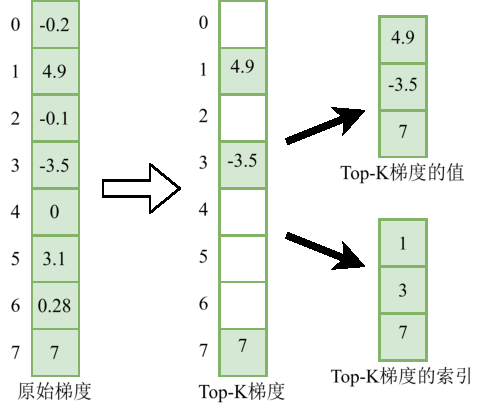
\includegraphics[height=0.53\textwidth]{Top-k.pdf}
    \caption{Top-K算法原理图}
    \label{fig_Top-k}
\end{figure}
%%%%%%%%%%%%%%%%%%%%%%%%%%%%%%%%%%%%%%%

2)\textbf{量化}:
梯度量化算法是将高精度梯度值量化为较小位宽的低精度值(浮点型或整型),并将量化后的梯度应用于各节点之间的通信操作 \cite{karimireddy2019error},原理如图 \ref{fig_Quantize}。
Seide等人 \cite{seide20141}在2014年凭借实验证明,1-bit量化方案仍然可以提供良好的性能,同时大大降低了分布式系统中的通信成本。
Wen等人 \cite{wen2017terngrad}在2017年提出了TernGrad(Ternary Gradient Compression)算法,该算法通过随机数生成器为该方案提供理论保证,以确保随机量化后的梯度(三个数值:-1,0,1)仍然是原梯度的无偏近似。
TernGrad不仅大大减少了通信时间,而且在梯度有界的前提下,其收敛性在数学上得到了证明,
但不幸的是,在大模型场景下,由于梯度方差极大膨胀,导致模型的准确度下降明显。
Alistarh等人 \cite{alistarh2017qsgd}通过探索数据并行化SGD中“通信成本”和“收敛保证”之间的关联性,提出了一系列有损压缩量化算法$\textbf{-}$量化随机梯度下降(Quantized Stochastic Gradient Descent, QSGD)。
在梯度数据方差的协助下,处理器可以通过该算法权衡每次迭代的通信数据比特数,但QSGD主要面向的是单机多GPU(Graphics Processing Unit)的分布式训练场景。
signSGD算法由Bernstein等人 \cite{bernstein2018signsgd}提出,是一种服务于分布式训练的量化方案,
该算法将每个计算节点的梯度值量化为二进制符号,然后主节点通过多数表决的方法对量化梯度进行汇总。
在神经网络模型分布式训练场景中,梯度通常用32-bit浮点数表示,因此用于梯度量化算法的压缩比上限为32。

%%%%%%%%%%%%%%%%%%%%%%%%%%%%%%%%%%%%%%%
\begin{figure}[htb]
    \centering
    \subfloat[二值化算法原理图]
        {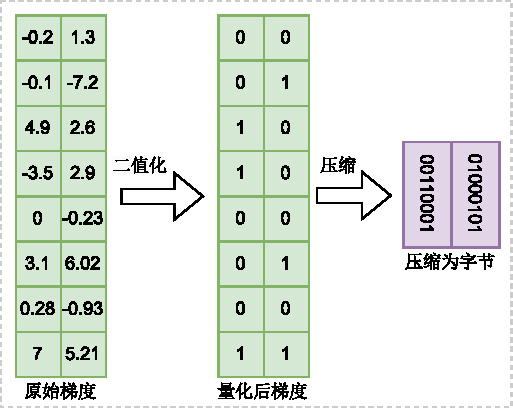
\includegraphics[width=0.50\linewidth]{量化原理图_a.pdf}}
    \subfloat[三值化算法原理图]
        {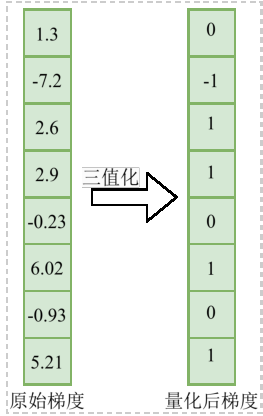
\includegraphics[width=0.252\linewidth]{量化原理图_b.pdf}}
    \caption{量化算法原理图}
    \label{fig_Quantize}
\end{figure}
%%%%%%%%%%%%%%%%%%%%%%%%%%%%%%%%%%%%%%%

3)\textbf{通信延迟}:
该类算法的思路是先在本地网络模型上进行数轮梯度更新,然后再与其他节点进行通信操作以实现全局梯度更新,从而降低各个节点之间的通信频率 \cite{chen2018lag},原理如图 \ref{fig_Communication} 所示。
McDonald等人 \cite{mcdonald2010distributed}和 Povey等人 \cite{povey2014parallel} 分别将局部迭代得到的平均梯度值应用于感知器和语音识别场景的DNN分布式训练。
Zhang等人 \cite{zhang2015deep}研究出了一种具有“弹性平均”的SGD异步方法。
McMahan等人 \cite{mcmahan2017communication}在2017年提出了联合平均算法(Federated Averaging),
该算法在每个计算节点的多次迭代步骤中执行SGD算法,并将多次迭代得到的局部梯度平均值用于网络通信,而非每次迭代获得的梯度值,从而大幅降低了各节点之间的通信频率。
实验表明,在不同的神经网络模型中,例如卷积神经网络(Convolutional Neural Network,CNN)和循环神经网络(Recurrent Neural Network,RNN),
局部迭代的通信延迟算法不仅没有显著降低网络模型的收敛速度,而且可以将必要的通信次数降低10~100倍。
%%%%%%%%%%%%%%%%%%%%%%%%%%%%%%%%%%%%%%%
\begin{figure}[htb]
    \centering
    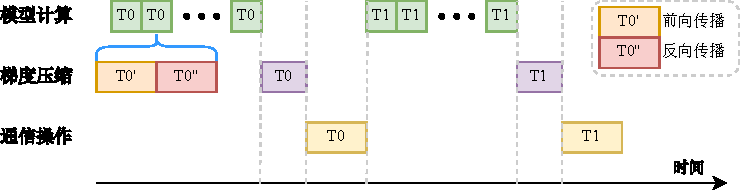
\includegraphics[width=0.9\textwidth]{通信延迟原理.pdf}
    \caption{分布式训练通信延迟算法原理图}
    \label{fig_Communication}
\end{figure}
%%%%%%%%%%%%%%%%%%%%%%%%%%%%%%%%%%%%%%%


%%%%%%%%%%%%%%%%%%%%%%%%%%%%%%%%%%%%%%%%%%%%%%%%%%%%%%%%%%%
%%%%%%%%%%%%%%%%%%%%%%%%%%%%%%%%%%%%%%%%%%%%%%%%%%%%%%%%%%%
\section{本文研究内容和章节安排}
\subsection{本文研究内容}
本文主要以大规模数据场景下进行高复杂网络模型的分布式训练为背景,深入学习和研究了各种梯度压缩算法,并对这些梯度压缩算法所面临的挑战进行了分析。
针对图像分类和高光谱目标检测等下游任务中分布式训练所面临的挑战和问题,
从梯度稀疏化以及通信延迟两个关键角度入手,展开了相关梯度压缩技术的深入研究,提出了以下两种高效的梯度压缩算法:

1)\textbf{基于近似质心的梯度压缩算法}

面对诸如高光谱目标检测等任务涉及到的大数据大模型场景时,传统单节点的计算资源、存储资源有限,难以满足部署、训练的要求。
而现有的分布式训练技术尽管可以部署、训练,但因高频、大流量、全尺寸全精度的通信行为,导致各节点之间的通信花销成为其关键瓶颈,从而大幅增加了训练时长。
因此,本文提出基于近似质心的梯度压缩算法(Gradient Compression via Approximate Centroid,GCAC),
该算法基于网络模型反向传播时梯度的近似质心,将网络模型中各梯度与近似质心的欧几里得范数作为距离度量,对模型中的梯度进行排序,
并在排序结果的基础上,利用Top-K算法选取合适的梯度用于通信操作,大幅压缩通信数据,显著降低了通信开销。

2)\textbf{基于$k$-互异近邻的梯度压缩算法}

压缩比较小的分布式训练场景中,现有的梯度稀疏化算法在整体训练速度和模型准确度都取得了不错的效果。
当期望分布式训练花费的时间进一步缩短时,自然而然的想法就是增加压缩比,进而大幅减少各节点之间通信操作数据量。
但这时,一些常见的梯度稀疏化算法(包括GCAC)都对模型的准确度产生了较大的影响,模型收敛性差,使得网络模型无法很好地发挥其优势。
针对大压缩比导致的模型收敛性差的情况,本文提出基于$k$-互异近邻的梯度压缩算法(Gradient Compression based on $k$-Reciprocal Nearest neighbors,$k$-RNGC),
该算法通过梯度计算感知与$k$-互异近邻选择算法相结合,优选出满足预设全局压缩比阈值的梯度,并协同动量修正和预热训练等组件,优化了分布式训练流程,显著降低了分布式训练过程中的网络通信数据量,大幅度加快了网络模型训练速度。

\subsection{本文章节安排}
围绕分布式训练和梯度压缩算法,本论文的具体结构组织以及各章节的主要内容描述如下:

第一章,绪论。
本章首先介绍了诸如高光谱遥感图像等大规模数据集的特点以及分布式训练的背景和意义。
然后,根据高光谱图像、超大规模自然图像等数据集的特点以及深度神经网络的发展现状,
深入分析了分布式训练在大规模数据集场景下训练高复杂度网络模型时所面临的挑战和问题。
接下来,对国内外现有的梯度压缩算法研究现状做了简要介绍和分析。
最后,阐述了本文的主要研究内容和章节安排。

第二章,相关理论基础。
本章介绍了深度学习基础、分布式训练基础、现有分布式平台介绍以及本文涉及的任务场景相关介绍。
首先,简要介绍了深度学习基础,深入分析并阐述了将分布式训练应用于大数据场景的必要性。
其次,简略介绍了分布式训练中的关键组件,包括分布式算法的实现方式、并行方式、同步方式等,同时介绍了现有的分布式平台。
最后,详细介绍了实验任务场景相关理论,包括高光谱目标检测和自然分类两个下游任务及其相关数据集和评测指标,为后续的实验设计和结果分析提供支撑。

第三章,基于近似质心的梯度压缩算法。
本章首先对网络模型中的局部梯度进行分析,深入探讨了局部梯度的分布特性,为后续算法设计打下基础。
然后,详细介绍了GCAC算法的相关理论,并给出了该算法应用于分布式训练的具体流程。
最后,在不同规模、不同类型的图像数据集上,通过在高光谱目标检测以及图像分类两大任务场景进行实验,
验证了该算法在分布式训练中的优势与不足,即在减少通信开销、提高训练效率等方面优势,以及面对大压缩比场景下的局限性。

第四章,基于$k$-互异近邻的梯度压缩算法。
首先,剖析了GCAC算法所面临的大压缩比难题,并指出导致该问题产生的原因,深入分析GCAC算法在大压缩比时所面临的挑战。
其次,详细介绍了$k$-RNGC算法的核心组件,包括局部梯度计算感知算法、$k$-互异近邻梯度选择算法、动量修正以及预热训练,并给出了各组件在分布式训练中应用流程。
然后,通过组件分析实验以及耗时分析实验,验证了$k$-RNGC算法核心组件的有效性以及必要性。
最后,在不同规模的数据集上实施了高光谱目标检测和图像分类实验,实验结果证实本章所提出算法的有效性和泛化性,充分展示了$k$-RNGC算法在实际应用中的潜力和优势。

第五章,总结与展望。本章一方面总结了论文的主要研究内容;另一方面,基于对梯度压缩算法的充分了解,提出了对未来工作的展望。


%%%%%%%%%%%%%%%%%%%%%%%%%%%%%%%%%%%%%%%%%%%%%%%%%%%%%%%%%%%
%%%%%%%%%%%%%%%%%%%%%%%%%%%%%%%%%%%%%%%%%%%%%%%%%%%%%%%%%%%
\chapter{相关理论基础}
\label{sec_chapter-2}
\section{引言}
目前以及将来的高光谱遥感图像数据,是数据规模非常大的3$\textbf{-}$D数据体,包括了空间位置信息和光谱信息。
HSI日益增加的数据规模对ML技术提出了更高的要求,尤其是在数据存储和处理方面,因此必须依赖足够大规模的并行/分布式训练技术。
值得注意的是,梯度压缩算法在大程度上推动了分布式训练技术的发展 \cite{song2021communication} \cite{ghosh2021communication} \cite{zhang2020communication} \cite{khirirat2020compressed}。
因此,为了便于后续研究本论文关注的梯度压缩算法,
本章首先介绍深度学习相关理论基础,紧接着对分布式理论基础进行阐述,
然后介绍高光谱目标检测、图像分类等下游任务场景,最后介绍与下游任务场景相关的实验数据集和性能评价指标。

\section{深度学习基础}
\subsection{网络模型架构介绍}
%%%%%%%%%%%%%%%%%%%%%%%%%%%%%%%%%%%%%%%
\begin{figure}[htb]
    \centering
    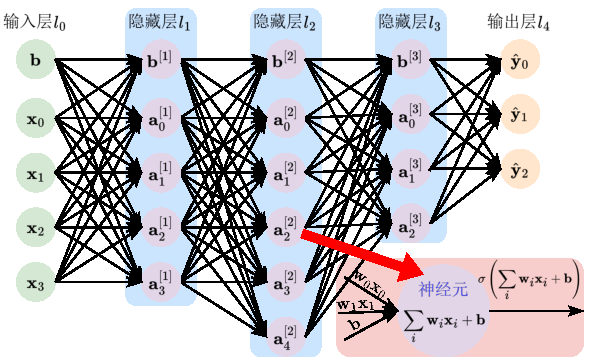
\includegraphics[width=0.98\textwidth]{神经网络结构.pdf}
    \caption{神经网络层级结构原理示意图}
    \label{fig_NetworkStruct}
\end{figure}
%%%%%%%%%%%%%%%%%%%%%%%%%%%%%%%%%%%%%%%

深度学习技术是机器学习领域的一个重要分支,
层级人工神经网络模型通常依照输入层、输出层以及大量隐藏层的网络结构搭建而成,
并堆叠了大量的非线性信息处理单元,凭借其网络结构对数据的表征、抽象能力强以及可执行任务灵活高的优势,被广泛应用于计算机视觉、自然语言处理等众多领域。
如图 \ref{fig_NetworkStruct} 所示,神经网络模型的每一层都包含大量相互连接的神经元(Neuron),而不同的神经网络架构正是体现在神经元连接方式和计算方式等方面的差异。
当输入数据通过神经网络时,网络模型中每一层神经元上的权重将会进行适当调整,即神经元被激活或抑制,从而产生相应的输出。
以卷积神经网络为例,与图 \ref{fig_NetworkStruct} 所示的全连接网络模型不同,CNN以卷积层作网络架构核心组件,
每一个卷积层都是由卷积计算单元、非线性计算单元以及可选的下采样变换单元构成,最后根据不同的下游任务选择合适的全连接层、分类器、检测器等后续组件。

在图 \ref{fig_NetworkStruct} 中,$\mathbf{X} = \{ \mathbf{x}_{0}, \mathbf{x}_{1}, ... , \mathbf{x}_{n^{[1]}} \}$表示输入数据,
$\mathbf{b}$为神经元偏置项(Bias),$\mathbf{a}$表示该神经元的激活值,
${\cdot}^{[l]}$用于表明当前层位于该网络模型中第$l$层,
$L$表示整个网络模型的总层数,
$n^{[l]}$表示第$l$层的神经元数量,
$\mathbf{w}_{i, j}^{[l]}$表示第$l-1$层中第$i$个神经元与第$l$层中第$j$个神经元之间的参数,
$\sigma(\cdot)$表示非线性激活函数(Activation Function)。

\subsection{激活函数简要介绍}
神经网络技术中,激活函数定义了该神经元在给定的输入或输入集合情况下的输出,即定义了神经网络输出的数学方程式,如图 \ref{fig_Delta} 展示了一些常见激活函数的曲线分布。

%%%%%%%%%%%%%%%%%%%%%%%%%%%%%%%%%%%%%%%
\begin{figure}[ht]
    \centering
    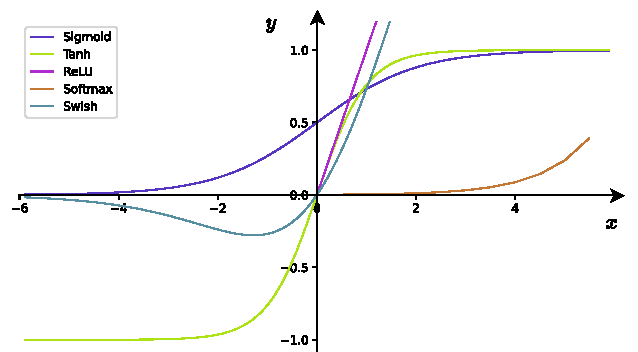
\includegraphics[width=0.86\textwidth]{delta.pdf}
    \caption{常见的激活函数曲线}
    \label{fig_Delta}
\end{figure}
%%%%%%%%%%%%%%%%%%%%%%%%%%%%%%%%%%%%%%%

Sigmoid激活函数,数学描述如公式 \eqref{eq_Sgimoid} 所示,该函数的输出区间为$(0, 1)$,相当于对每个神经元的输出进行归一化,常用于预测概率模型和神经网络的输出层。
%%%%%%%%%%%%%%%%%%%%%%%%%%%%%%%%%%%%%%%
\begin{equation}
    \sigma_{Sigmoid}\left( x \right) = \frac{1}{1+e^{-x}}
    \label{eq_Sgimoid}
\end{equation}
%%%%%%%%%%%%%%%%%%%%%%%%%%%%%%%%%%%%%%%

双曲正切(Tanh)激活函数,如公式 \eqref{eq_Tanh} 所示,输出区间为$(-1, 1)$,且当输入较大或较小时,保证输出平滑的同时,梯度较小,常用于隐藏层。
%%%%%%%%%%%%%%%%%%%%%%%%%%%%%%%%%%%%%%%
\begin{equation}
    \sigma_{Tanh}\left( x \right) = \frac{e^{x}-e^{-x}}{e^{x}+e^{-x}}
    \label{eq_Tanh}
\end{equation}
%%%%%%%%%%%%%%%%%%%%%%%%%%%%%%%%%%%%%%%

如公式 \eqref{eq_ReLU} 所示的ReLU激活函数,在深度学习领域中较为流行。
当输入为正时,不存在梯度饱和的问题,且只存在线性关系,计算速度更快。
但当输入为负,反向传播时梯度恒为零,ReLU激活函数完全失效。
%%%%%%%%%%%%%%%%%%%%%%%%%%%%%%%%%%%%%%%
\begin{equation}
    \sigma_{ReLU}\left( x \right) = 
        max(0, x) = 
            \begin{cases}
                0 & \text{if } x < 0,\\
                x & \text{if } x \ge 0.
            \end{cases}
    \label{eq_ReLU}
\end{equation}
%%%%%%%%%%%%%%%%%%%%%%%%%%%%%%%%%%%%%%%

Softmax激活函数,如公式 \eqref{eq_Softmax} 所示,该函数的输出范围为$(0, 1)$,且输出是总和为$1$的$n^{[L]}$维实向量。
该激活函数的分母结合了原始输出值的所有因子,因此可认为是$argmax$函数的概率版本。
但该激活函数零点不可微,且当输入为负时梯度为零,常用于多分类问题。
%%%%%%%%%%%%%%%%%%%%%%%%%%%%%%%%%%%%%%%
\begin{equation}
    \sigma_{Softmax}\left( x_{i} \right) = 
        \frac{e^{x_{i}}}{\sum_{t = 1}^{n^{[L]}}e^{x_{t}}}, \quad i = 1, \dots, n^{[L]}
    \label{eq_Softmax}
\end{equation}
%%%%%%%%%%%%%%%%%%%%%%%%%%%%%%%%%%%%%%%

Swish激活函数,如公式 \eqref{eq_Swish} 所示,其设计思路受到了长短期存储器(Long Short-term Memory,LSTM)和高速网络中 Gating的Sigmoid函数使用的启发。
当$\rho$为1时,激活函数曲线如图 \ref{fig_Delta} 所示。
该激活函数能够轻松替换以单个标量为输入的激活函数(例如ReLU),且无需修改隐藏容量或参数数量。
Swish的“无界”特性有助于防止产生慢速训练期间梯度逐渐接近0的问题,并且该激活函数的平滑度在优化和泛化中起到了重要作用。
%%%%%%%%%%%%%%%%%%%%%%%%%%%%%%%%%%%%%%%
\begin{equation}
    \sigma_{Swish}\left( x \right) = x * Sigmoid(\rho x)
    \label{eq_Swish}
\end{equation}
%%%%%%%%%%%%%%%%%%%%%%%%%%%%%%%%%%%%%%%


\subsection{网络模型训练流程介绍}
\label{sec_ModelTrainProduce}
深度学习技术尽管可以根据数据集是否具有标签信息划分为有监督和无监督两种训练范式,但是二者都对应数学上的凸优化问题。
然而,无论是无约束条件的凸优化问题还是有约束条件的凸优化问题,都可以通过引入拉格朗日函数转换成无约束条件的凸优化问题 \cite{chen1985optimize}。
因此,神经网络模型训练过程本质上就是求解一个无约束条件的凸优化问题的过程,如公式 \eqref{eq_Convex} 所示:
%%%%%%%%%%%%%%%%%%%%%%%%%%%%%%%%%%%%%%%
\begin{equation}
    \mathbf{\hat{W}} = \arg\min_{\mathbf{W}}{\mathcal{L} \left(\mathbf{X; W} \right)}
    \label{eq_Convex}
\end{equation}
%%%%%%%%%%%%%%%%%%%%%%%%%%%%%%%%%%%%%%%
其中,$\mathbf{X}$表示输入数据,$\mathcal{L}$通常被称为损失函数(Loss Function),
例如平均绝对误差(Mean Absolute Error,MAE)、均方误差(Mean Square Error,MSE)、交叉熵(Cross Entropy,CE)等。

整个训练过程不断通过前向传播(Forward)、反向传播(Backforward Propagation,BP)等步骤的交替迭代进行,以实现模型参数矩阵$\mathbf{W}$的最优值求解,如图 \ref{fig_SignleNodeUpdateAlgo} 所示,其中的核心步骤描述如下:

%%%%%%%%%%%%%%%%%%%%%%%%%%%%%%%%%%%%%%%
\begin{figure}[t]
    \centering
    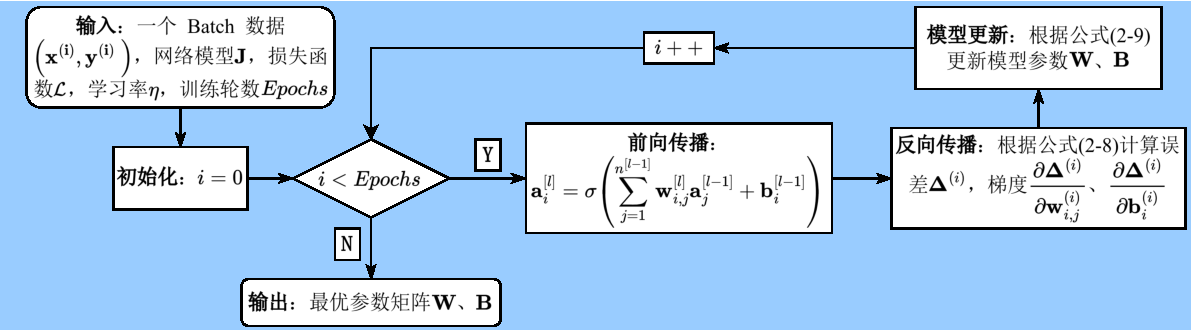
\includegraphics[width=0.98\linewidth]{SGD-Algorithm-单节点SGD.pdf}
    \caption{单节点网络模型SGD训练流程}
    \label{fig_SignleNodeUpdateAlgo}
\end{figure}
%%%%%%%%%%%%%%%%%%%%%%%%%%%%%%%%%%%%%%%

1)\textbf{初始化网络模型参数}:对网络模型中的参数矩阵$\mathbf{W}$和偏置项$\mathbf{b}$进行初始化,可采用包括随机初始化、零值初始化、特征初始化等初始化方式。

2)\textbf{前向传播}:将训练数据$\mathbf{X}$输入到网络中,
并依据
$\textbf{\mbox{输入层}} \Rightarrow \textbf{\mbox{隐藏层}} \Rightarrow \textbf{\mbox{输出层}}$
的网络结构依次计算各层神经元的激活值$\mathbf{a}_{i}^{[l]}$,并进一步求得实际输出$\hat{\mathbf{Y}}$,
如公式 \eqref{eq_a_l_i} 所示:
%%%%%%%%%%%%%%%%%%%%%%%%%%%%%%%%%%%%%%%
\begin{equation}
    \mathbf{a}_{i}^{[l]} =
        \sigma \left( \sum_{j = 1}^{n^{[l-1]}}{\mathbf{w}_{i, j}^{[l]}\mathbf{a}_{j}^{[l - 1]} + \mathbf{b}_{i}^{[l - 1]}} \right)
    \label{eq_a_l_i}
\end{equation}
%%%%%%%%%%%%%%%%%%%%%%%%%%%%%%%%%%%%%%%

3)\textbf{反向传播}:与前向传播相比,该步骤数据流的方向恰恰相反,即依据
$\textbf{\mbox{输出层}} \Rightarrow \textbf{\mbox{隐藏层}} \Rightarrow \textbf{\mbox{输入层}}$
的方向,并根据预先定义的损失函数计算实际输出$\hat{\mathbf{y}}$与目标$\mathbf{y}$之间的误差值$\mathbf{\Delta}$,
然后采用链式求导规则计算每一层的梯度$\mathbf{g}$,如公式 \eqref{eq_Partial} 所示:

% \textcolor{red}{FIXME: 求解梯度是应该是$\prod_{k = 1}^{n^[l+1]}{\left(\frac{\partial \mathbf{\Delta}}{\partial \mathbf{a}_{k}^{[l+1]}}\frac{\partial \mathbf{a}_{k}^{[l+1]}}{\partial \mathbf{a}_{i}^{[l]}}\right)\frac{\partial \mathbf{a}_{i}^{[l]}}{\partial \mathbf{w}_{i, j}^{[l]}}}$}

%%%%%%%%%%%%%%%%%%%%%%%%%%%%%%%%%%%%%%%
\begin{equation}
    \begin{aligned}
        \mathbf{\Delta} & = 
        \mathcal{L}_{MSE}\left( \mathbf{\hat{Y}}, \mathbf{Y} \right) = \frac{1}{M} \sum_{m =
        1}^{M} {\sum_{i = 1}^{n^{[L]}}{\left(\mathbf{\hat{y}}_{i}^{[L]} - \mathbf{y}_{i} \right) ^{2}} }\\
        \mathbf{g}\left( \mathbf{w}_{i, j}^{[l]} \right) & =
        \frac{\partial \mathbf{\Delta}}{\partial \mathbf{w}_{i, j}^{[l]}} = 
        \frac{\partial \mathbf{\Delta}}{\partial \mathbf{a}_{i}^{[l]}} 
        \frac{\partial \mathbf{a}_{i}^{[l]}}{\partial \mathbf{w}_{i, j}^{[l]}} =
        \left(
            \sum_{k = 1}^{n^{[l+1]}}{
                \frac{\partial \mathbf{\Delta}}{\partial \mathbf{a}_{k}^{[l+1]}}
                \frac{\partial \mathbf{a}_{k}^{[l+1]}}{\partial \mathbf{a}_{i}^{[l]}}
            } 
        \right)
        \frac{\partial \mathbf{a}_{i}^{[l]}}{\partial \mathbf{w}_{i, j}^{[l]}} \\
        \mathbf{g}\left( \mathbf{b}_{i, j}^{[l]} \right) & = 
        \frac{\partial \mathbf{\Delta}}{\partial \mathbf{b}_{i}^{[l]}} = 
        \frac{\partial \mathbf{\Delta}}{\partial \mathbf{a}_{i}^{[l]}} 
        \frac{\partial \mathbf{a}_{i}^{[l]}}{\partial \mathbf{b}_{i}^{[l]}} =
        \left(
            \sum_{k = 1}^{n^{[l+1]}}{
                \frac{\partial \mathbf{\Delta}}{\partial \mathbf{a}_{k}^{[l+1]}}
                \frac{\partial \mathbf{a}_{k}^{[l+1]}}{\partial \mathbf{a}_{i}^{[l]}}
            } 
        \right)
        \frac{\partial \mathbf{a}_{i}^{[l]}}{\partial \mathbf{b}_{i}^{[l]}}
    \label{eq_Partial}
    \end{aligned}
\end{equation}
%%%%%%%%%%%%%%%%%%%%%%%%%%%%%%%%%%%%%%%
其中,$M$为目标种类数量,$\mathbf{g}\left( \mathbf{w}^{[l]} \right)$和$\mathbf{g}\left( \mathbf{b}^{[l]} \right)$表示第$l$层神经元相关梯度,为了方便后续描述以及公式清晰化,相关梯度将简化表示为$\mathbf{g}^{[l]}$。

4)\textbf{网络模型参数更新}:基于公式 \eqref{eq_Partial} 求得的梯度,结合预设的优化算法(如SGD、Adagrad、Adam等)完成各层神经元的参数更新。
以SGD优化算法为例,网络模型参数更新如公式 \eqref{eq_Updata} 所示:
%%%%%%%%%%%%%%%%%%%%%%%%%%%%%%%%%%%%%%%
\begin{equation}
    \begin{aligned}
        \mathbf{w}_{i, j}^{[l]} &=
        \mathbf{w}_{i, j}^{[l]} - \eta \frac{\partial \mathbf{\Delta}}{\partial \mathbf{w}_{i, j}^{[l]}}\\
        \mathbf{b}_{i}^{[l]} &=
        \mathbf{b}_{i}^{[l]} - \eta \frac{\partial \mathbf{\Delta}}{\partial \mathbf{b}_{i}^{[l]}}
        \label{eq_Updata}
    \end{aligned}
\end{equation}
%%%%%%%%%%%%%%%%%%%%%%%%%%%%%%%%%%%%%%%
其中,$\eta$表示模型训练过程中的学习率(Learning Rate,LR)。

5)\textbf{迭代}:重复步骤2)至步骤4),直至满足预设条件或模型收敛,输出最优参数矩阵。


\section{分布式训练理论基础}
结合大数据时代以及神经网络模型训练过程,不难发现,整个训练过程涉及到的数据量、计算量都非常大。
在理论层面再次表明,现在以及将来的深度学习训练场景必然对设备存储、计算等要求暴增。
无论是总线拓扑(单机多GPU)还是网状/星型拓扑(多机多GPU)的多设备并行/分布式训练,
不仅满足存储和计算要求,而且在理论上不借助其他算法就可以加速网络训练速度,
可以极大程度地发挥深度学习的优势,必将成为主流训练范式。

分布式训练是一种采用“分而治之”思想的训练技术。该训练技术将一个训练任务分配到多个计算节点上进行并行计算,旨在提高模型训练速度和模型质量。
该技术已被广泛应用于深度学习领域,尤其是面对于大规模数据集和复杂的网络模型,
例如超大规模自然图像处理、高光谱目标检测、自然语言处理等众多任务领域 \cite{JFYZ202101008}。
另外,目前常见的DL框架\cite{abadi2016tensorflow} \cite{ketkar2021introduction} \cite{jia2014caffe} \cite{gulli2017deep} \cite{seide2016cntk}均已支持分布式训练,可见其发展势头之猛。

分布式训练过程通常会协同多张GPU,以提供足够的显存、计算能力以及并行度,极大程度提高训练速度。
分布式算法的核心思路是将一个任务划分为多个小型任务进行并行计算。
详细地说,分布式训练是首先基于分布式网络拓扑架构,将一个大型的计算任务划分为许多小型任务,并交由相应的节点完成并行计算,
然后在各计算节点之间采用同步算法进行聚合、更新,以确保本次迭代过程中有效节点的计算结果都成功用于模型梯度、参数更新,重复迭代整个训练过程直至模型收敛。
需要注意的是,计算节点对应的是计算机中的进程,而各个进程并不要求与硬件设备一一对应,
也就是说多个节点可以部署在同一台设备上(即单机多GPU拓扑),也可以部署在多台设备上(即多机多GPU拓扑)。

接下来本章各小节将对分布式训练的并行方式、设备拓扑架构、各节点之间的同步更新方式以及现有分布式平台等方面进行深入介绍。

\subsection{分布式训练的并行方式}
\label{sec_DistributedParallsim}
目前,从并行方式的角度出发,现有的分布式训练技术主要有以下几种实现方式:1)数据并行(Data Parallelism) \cite{li2020pytorch}、2)模型并行(Model Parallelism) \cite{shoeybi2019megatron}、3)流水线并行(Pipeline Parallelism) \cite{huang2019gpipe}。

%%%%%%%%%%%%%%%%%%%%%%%%%%%%%%%%%%%%%%%
\begin{figure}[htb]
    \centering
    \subfloat[数据并行]{
        % \includegraphics[width=0.33\linewidth]{分布式并行方式-数据并行.pdf}
        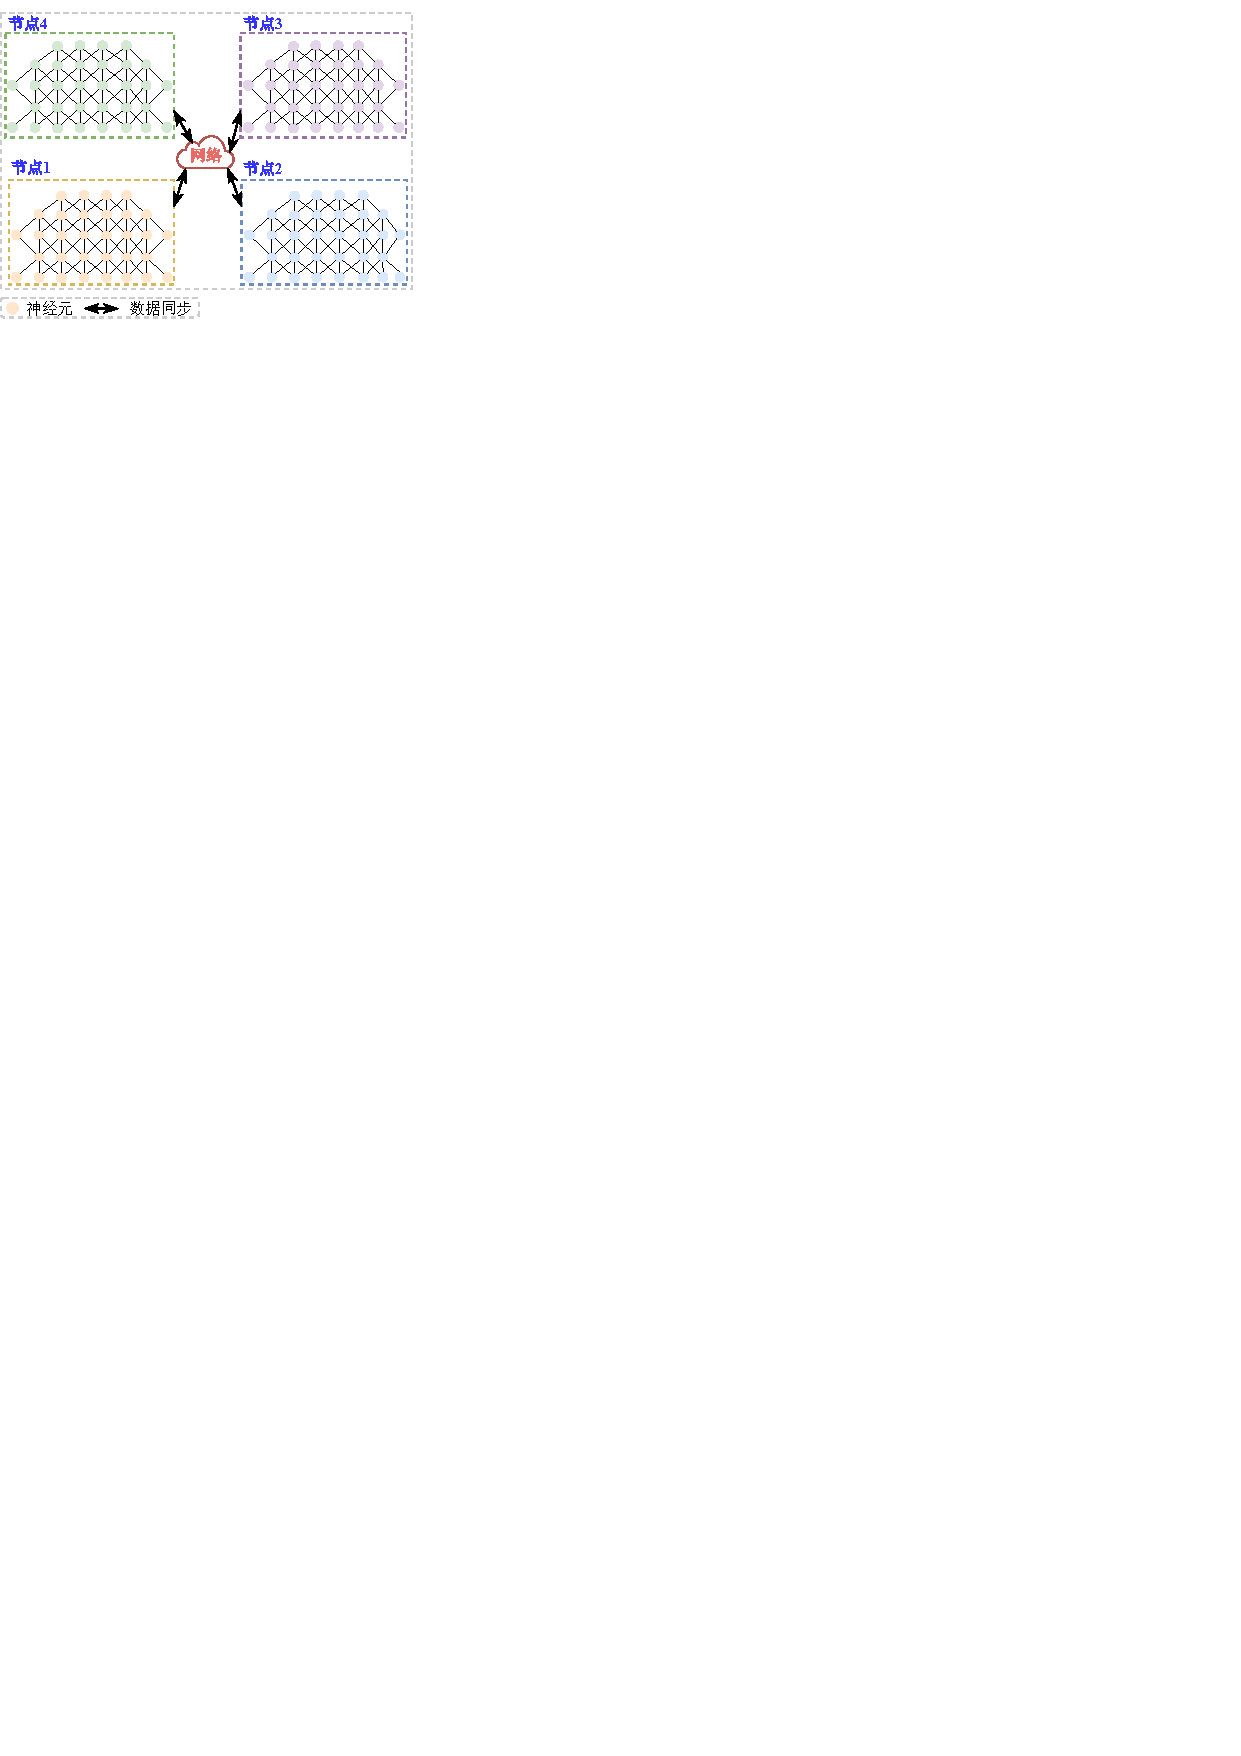
\includegraphics[width=0.33\linewidth]{分布式并行方式-数据并行-v2.pdf}
        \label{fig_DataParallelism}
    }
    \subfloat[模型并行]{
        % \includegraphics[width=0.40\linewidth]{分布式并行方式-模型并行.pdf}
        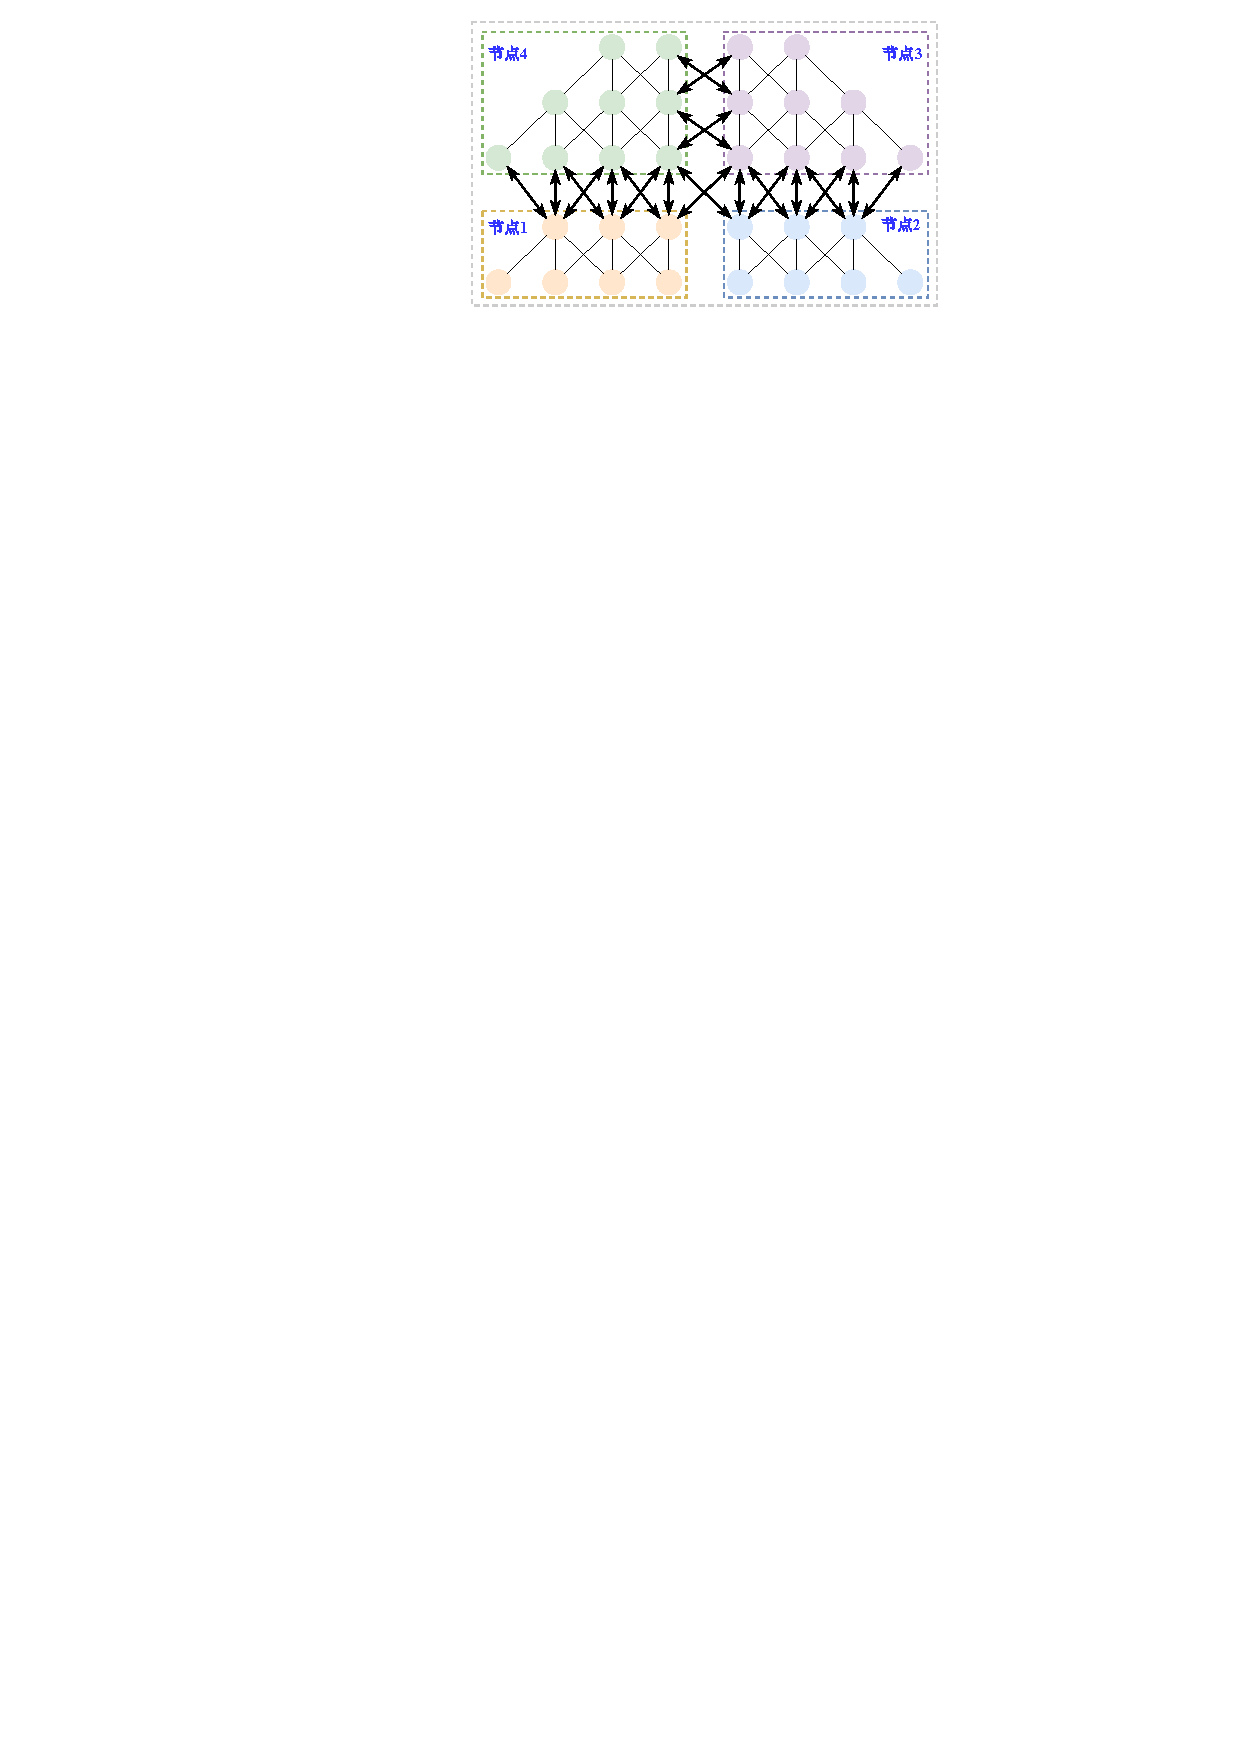
\includegraphics[width=0.40\linewidth]{分布式并行方式-模型并行-v2.pdf}
        \label{fig_ModelParallelism}
    }
    \subfloat[流水线并行]{
        % \includegraphics[width=0.22\linewidth]{分布式并行方式-流水线并行.pdf}
        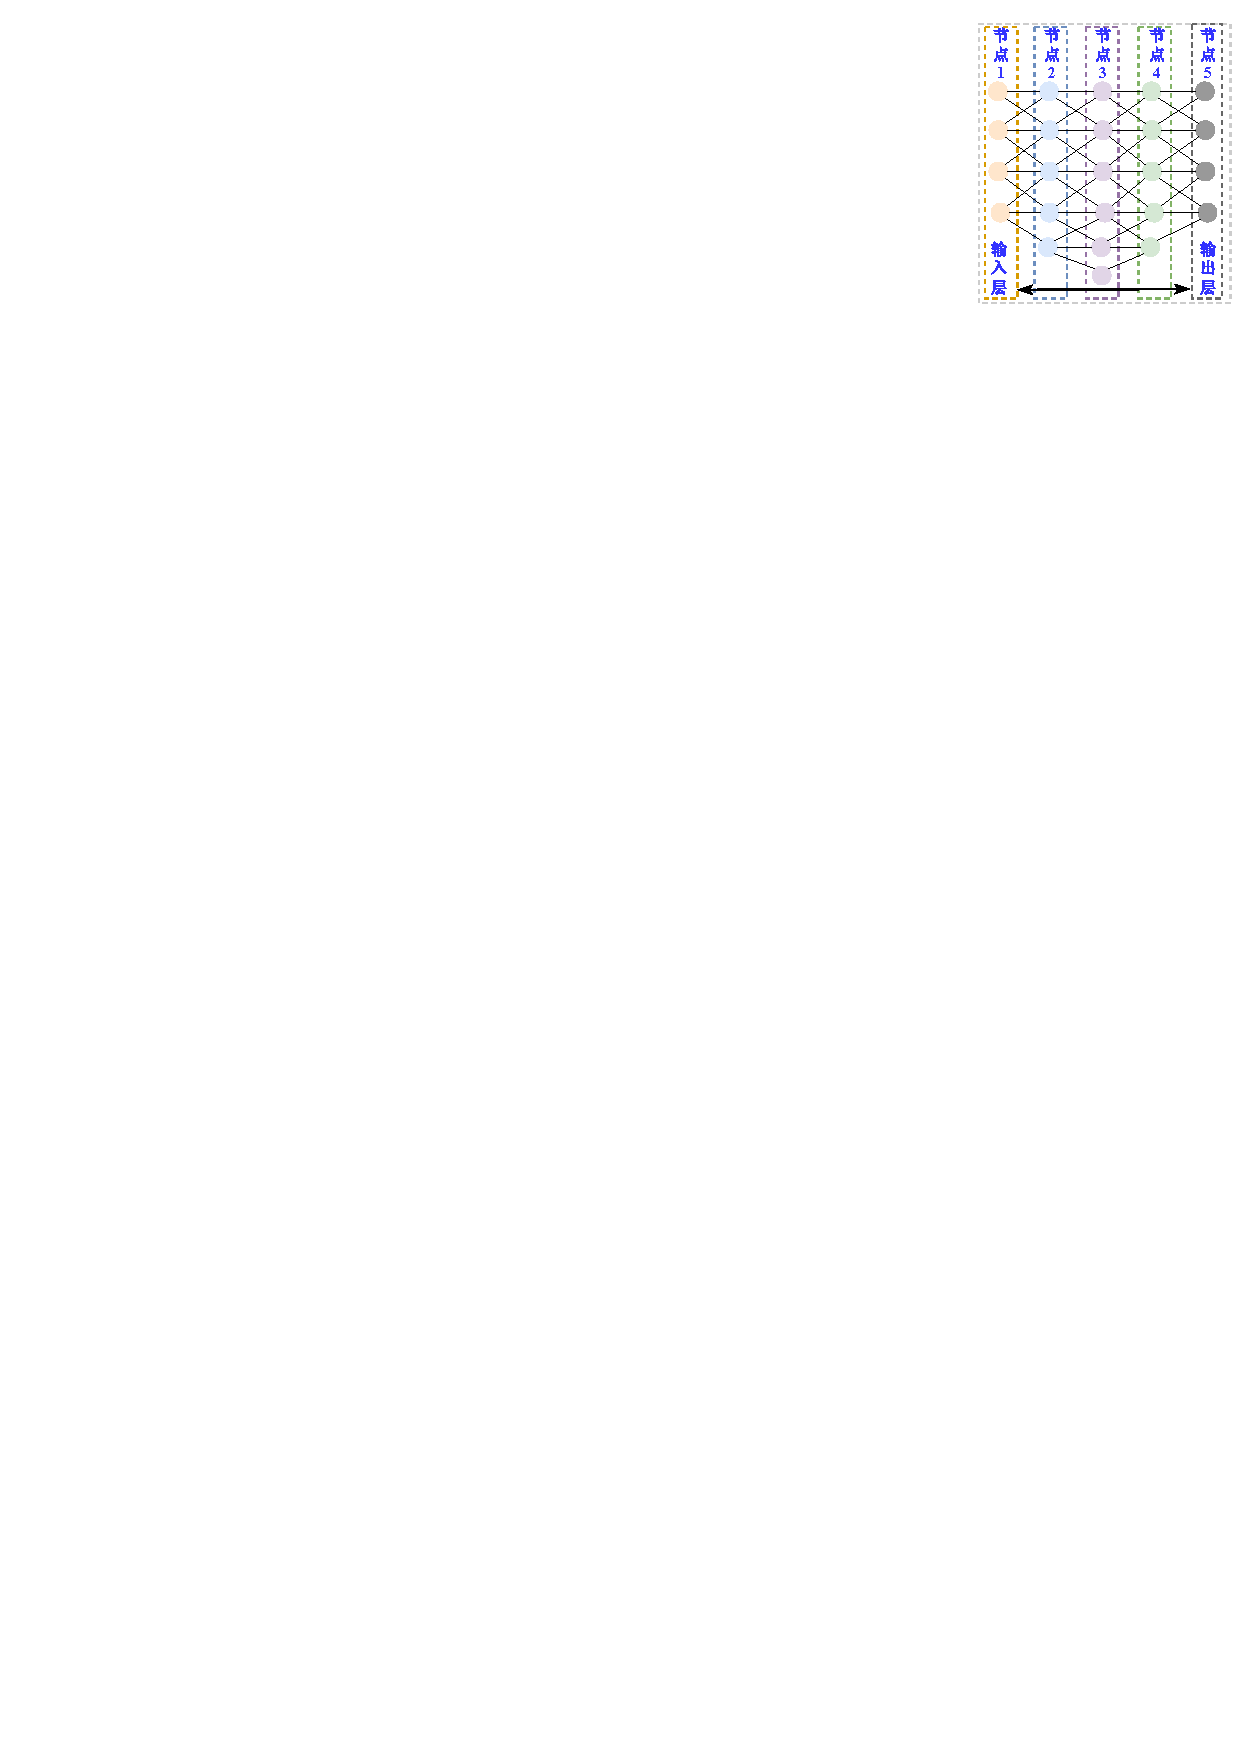
\includegraphics[width=0.22\linewidth]{分布式并行方式-流水线并行-v2.pdf}
        \label{fig_PipelineParallelism}
    }
    \caption{数据并行、模型并行和流水线并行示意图}
    \label{fig_Parallelism}
\end{figure}
%%%%%%%%%%%%%%%%%%%%%%%%%%%%%%%%%%%%%%%

1)\textbf{数据并行}:众所周知,用于训练的数据量越大,神经网络模型的效果越好,但如今单计算节点显存往往不足以存储日益增加的数据。
自然而然的解决方案就是将海量数据进行分割并分配到各个计算节点,让每个节点只负责训练本地的子数据集,这种划分数据集进行并行计算的训练模式就是数据并行,如图 \ref{fig_Parallelism} \subref{fig_DataParallelism} 所示。
后来逐渐发展成为一种广泛应用于深度学习技术领域的学习范式。
在网络模型被完整部署到每个计算节点的前提下,数据并行将超大规模的数据集进行随机且均匀地分割成多个子数据集,
每个计算节点只需负责训练被分配到的本地子数据集,然后与其余计算节点进行网络模型信息的同步以及更新。

由 \ref{sec_ModelTrainProduce} 小节介绍可知,
网络模型的整个训练过程是一个不断迭代执行的过程,也就意味着整个练过程将会进行大量迭代,
同时模型的参数矩阵正是在每次迭代中逐渐优化,而每次迭代都需要在节点之间传输大量数据(模型权重和/或梯度),势必会拖慢网络模型的整体训练节奏。
总之,数据并行在实际应用中也面临着巨大的挑战:
第一,现在以及将来的神经网络模型体积越来越大,网络参数爆炸式增长,导致分布式训练梯度同步过程中的通信数据量越来越多,逐渐成为限制模型训练的关键因素。
第二,近几年,GPU和其他神经网络加速器等设备的计算能力取得到了飞跃式的进步,
但用于各计算节点之间的网络设备带宽的发展相对迟缓 \cite{gholami2021ai}。
这意味着,算力提升与网络带宽之间的发展不匹配,导致计算节点的计算能力无法完全用于提升网络模型的训练速度,最终将会使得网络通信的瓶颈问题暴露愈加明显。

2)\textbf{模型并行}:
大型深度学习网络模型,通常包含数百万甚至数十亿个参数,如表 \ref{tab_LargeScaleModelParams} 所示。
当使用GPU进行网络模型训练加速时,由于单个计算节点上的GPU显存总是受限,往往无法将网络模型中的参数矩阵和梯度矩阵以及用于前向传播、反向传播时的辅助变量全部加载到显存中。
例如,Nvidia公司推出的GeForce RTX 2080Ti GPU采用Truing架构,有效显存只有11GB,显然易见,
当神经网络模型体积、参数量过大时,单节点单GPU的情形下可能需要数天或数周时间,甚至连模型都可能无法顺利部署。

%%%%%%%%%%%%%%%%%%%%%%%%%%%%%%%%%%%%%%%
\renewcommand{\arraystretch}{1.3}
\begin{table*}[ht]
    \centering
    \caption{常见大规模深度学习网络模型参数}
    \label{tab_LargeScaleModelParams}
    \resizebox{\linewidth}{!}{
        \begin{tabular}{c|cccccccc}
            \toprule
            \toprule
                模型 & ResNet-50 & VGGNet-19 & ELMo & BERT-Base & BERT-Large & GPT-2 Large & GPT-2 XL & GPT-3 \\
            \midrule
                参数量(亿) & 0.256 & 1.43 & 0.078 & 1.1 & 3.4 & 7.75 & 15 & 1750 \\
            \bottomrule
            \bottomrule
        \end{tabular}}
\end{table*}
%%%%%%%%%%%%%%%%%%%%%%%%%%%%%%%%%%%%%%%

为了解决该问题,将大规模网络模型进行划分的训练模式被提出,让每一个计算设备仅仅负责管理、训练被分配到的部分模型,为大规模神经网络的训练提供一种可行方案,也就是模型并行,如图 \ref{fig_Parallelism} \subref{fig_ModelParallelism}  所示。
模型并行根据训练集群中的计算节点数量将整个模型进行切分,
每一个单独的计算节点将部署一个部分模型,并负责训练整个数据集。
多个计算节点并发执行,并定期与其他节点交换信息以更新模型。
通过使用模型并行的训练策略,不仅能够使超大规模的网络模型如期部署,而且还可以大幅缩短分布式训练时间。

3)\textbf{流水线并行}:Google最初在GPipe \cite{huang2019gpipe} 提出流水线并行。
该并行方式将分布式训练过程中的计算任务划分为多个阶段,
然后将这些阶段任务分配给不同的计算节点进行并行训练,以此来减少模型训练时的显存占用,
如图 \ref{fig_Parallelism} \subref{fig_PipelineParallelism}  所示。
PipeDream \cite{harlap2018pipedream} 由MicroSoft提出,
通过模型参数的异步更新以及1F1B调度策略减少并行气泡。
由于1F1B尽早释放占用内存,因此在内存占用方面优于GPipe,但同样可能存在模型不收敛以及内存膨胀的问题。
近年来,DAPPLE \cite{fan2021dapple} 在于1F1B之基础上采用模型参数同步更新,巧妙地避开了这些问题。
另外,分布式并行计算训练场景中,由于不同的计算节点之间需要交换数据进行同步,增加了通信开销,
而通信开销大小取决于训练数据集的规模和网络模型的复杂程度,流水线并行策略对于小规模分布式训练可能不会带来明显的性能提升。

尽管分布式训练的三种并行策略各有长短,但在深度学习技术领域的训练场景中,数据并行策略可保证神经网络模型快速收敛,实现简单,额外的性能开销相对不大且扩展性极强,应用范围最为广泛,逐渐成为分布式训练的主流范式。
因此,本文将重点关注数据并行策略下的梯度压缩技术研究。

\subsection{分布式训练的拓扑架构}
本文 \ref{sec_DistributedParallsim} 小节介绍了数据并行策略,规定了输入数据的划分方式,但没有描述分布式训练场景中的各个计算节点之间的网络拓扑。
根据网络中各计算节点的通信拓扑结构,数据并行策略下的分布式训练架构主要分为以下两种:
1)中心化的参数服务器(Parameter Server,PS)拓扑架构,如图 \ref{fig_DistributedStruct} \subref{fig_ParamterServerStruct} 所示;
2)去中心化的Collective架构,如图 \ref{fig_DistributedStruct} \subref{fig_CollectiveStruct} 所示。

%%%%%%%%%%%%%%%%%%%%%%%%%%%%%%%%%%%%%%%
\begin{figure}[ht]
    \centering
    \subfloat[参数服务器架构]{
        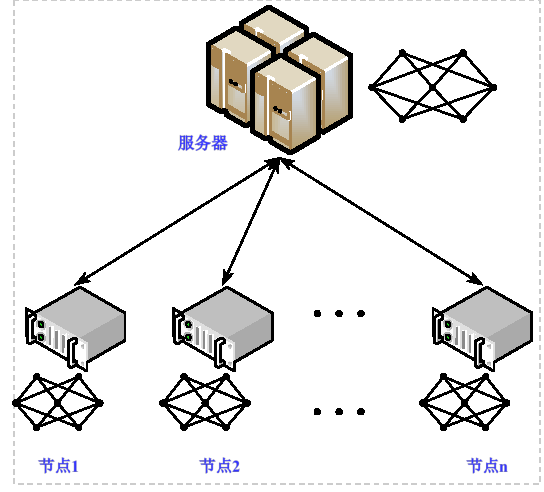
\includegraphics[width=0.40\linewidth]{分布式拓扑-服务器架构.pdf}
        \label{fig_ParamterServerStruct}
    }
    \subfloat[Collective架构]{
        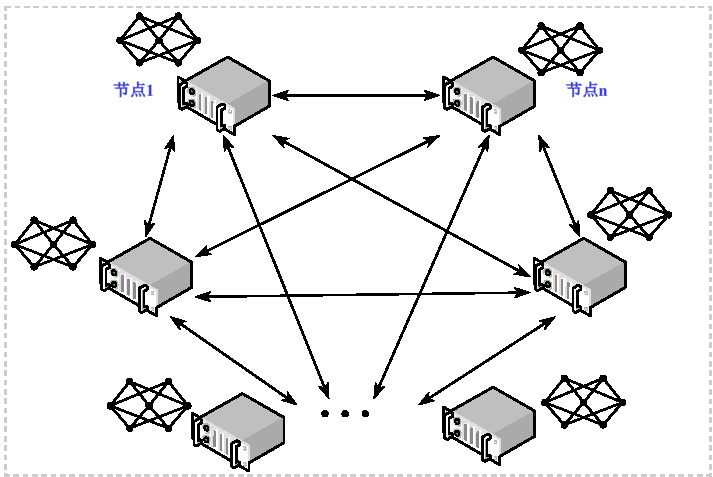
\includegraphics[width=0.548\linewidth]{分布式拓扑-Collective架构.pdf}
        \label{fig_CollectiveStruct}
    }
    \caption{数据并行策略下分布式训练场景中不同的通信拓扑架构 \cite{tang2020communication}}
    \label{fig_DistributedStruct}
\end{figure}
%%%%%%%%%%%%%%%%%%%%%%%%%%%%%%%%%%%%%%%

1)\textbf{参数服务器架构}:
参数服务器架构\cite{li2014scaling}是一种中心化(Centralized)的分布式训练通信拓扑,它通常由一个服务器(Server)和若干计算节点(Worker)构成,此时便构成了星型拓扑结构。
另外,当采用这种星型拓扑架构时,各个Worker之间相互隔离,不会发生数据交换操作,只会与Server之间通过拉取(Pull)和推送(Push)通信原语的方式进行数据交换。
% 图 \ref{fig_DistributedStruct}\subref{fig_ParamterServerStruct}展示了多机多节点的PS拓扑示意图。

在参数服务器网络拓扑中,Server持有整个神经网络模型的全部参数,负责参数的分片存储和更新;
Worker持有模型网络结构,根据分配到的子训练数据集进行模型前向传播和反向传播的并行计算,
得到网络模型对应的参数和梯度,分布式训练的大致过程如图 \ref{fig_DistributedUpdateAlgo} \subref{fig_ParameterServerTrain} 所示。
Worker每经过一次迭代训练,都可以向Server发送数据交换请求,获取网络模型的最新参数,然后基于该参数计算当前训练子数据集的梯度,择机推送给服务器;
Server等待所有Worker推送完毕后进行梯度聚合,然后采用SGD等优化算法进行全局参数更新。

参数服务器网络通信架构的优势有:
1)实现简单、原理清晰易于理解;
2)支持在不重启全部设备的情况下,动态更新Worker的数量;
3)同时支持分布式网络模型的同步训练和异步训练,能够缓解因某个Worker计算过慢而导致的同步时间过长问题。关于分布式训练过程中的网络模型的同步/异步更新将在本章的下一小节进行详细介绍。

%%%%%%%%%%%%%%%%%%%%%%%%%%%%%%%%%%%%%%%
\begin{figure}[t]
    \centering
    \subfloat[参数服务器架构]{
        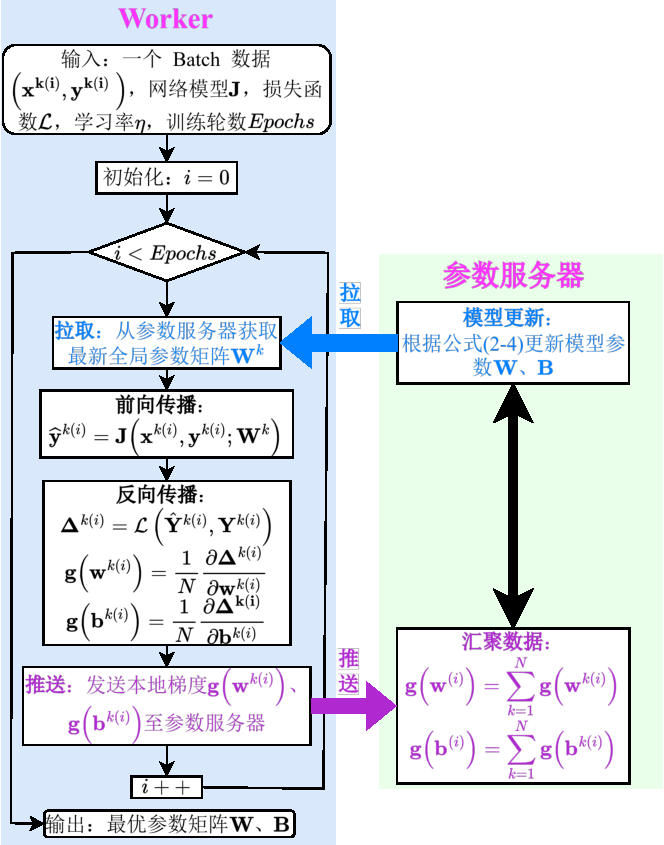
\includegraphics[width=0.63\linewidth]{SGD-Algorithm-参数服务器架构同步SGD.pdf}
        \label{fig_ParameterServerTrain}
    }
    \subfloat[Collective架构]{
        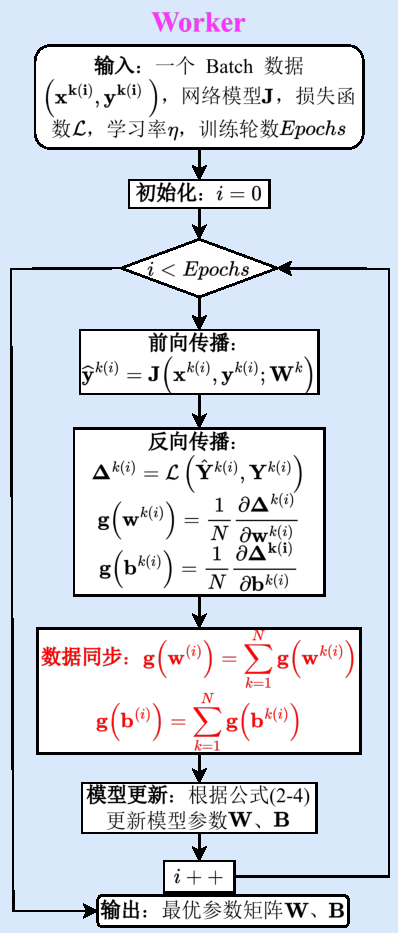
\includegraphics[width=0.34\linewidth]{SGD-Algorithm-Collective架构同步SGD.pdf}
        \label{fig_CollectiveTrain}
    }
    \caption{不同拓扑架构下同步更新的网络模型训练流程}
    \label{fig_DistributedUpdateAlgo}
\end{figure}
%%%%%%%%%%%%%%%%%%%%%%%%%%%%%%%%%%%%%%%

2)\textbf{Collective架构}:
参数服务器网络通信架构致命缺点是,随着Worker数量的增加,Server与各个Worker之间的网络通信带宽受限问题暴露的愈加明显,严重阻碍了分布式训练的速度,该问题被称为通信瓶颈。
为了解决该问题,仅仅通过增加Server的数量并不一定能够可行,因为目前主流的启发式的参数划分方案仍可能导致各个Server的任务负载不均衡 \cite{chen2020elastic},从而导致多对一的通信瓶颈问题。

目前,解决了参数服务器网络拓扑架构中通信瓶颈问题的方案是去中心化(Decentralized)的Collective架构。
在该架构中,没有模型参数管理Server,每一个Worker都是平等的,都持有网络模型的最新全局信息,执行相同的工作,
但各个Worker之间需要通过多次通信操作,以实现梯度同步,并且网络通信时需要使用Allreduce原语。

聚合通信,来源于HPC(High Performance Computing)领域的消息传递接口(Message Passing Interface,MPI)技术,它能够在多个进程之间进行高效通信,被广泛用于大规模数值计算领域,包括流体力学模拟、天气预报等。
Allreduce则是众多聚合通信原语(Reduce、Scatter、Allreduce、Allgather等)中的一种,它支持所有Reduce规则运算,包括求和、求平均值以及求最值等。
在数据并行策略的分布式训练过程中,使用Allreduce原语对网络模型的梯度、参数等信息进行聚合操作, 可以大幅改善其训练速度。

图 \ref{fig_DistributedUpdateAlgo} \subref{fig_CollectiveTrain} 
展示了基于Allreduce通信原语的数据并行策略下的分布式训练过程:
首先,Worker加载网络模型并读取子训练数据集,并进行前向、反向传播,获取局部梯度;
然后,各Worker通过Allreduce原语实现梯度聚合、交换,得到最新全局梯度;
最后,各Worker基于最新全局梯度进行模型参数更新,进入下一次迭代训练过程。

Allreduce原语在MPI技术中仅仅被规定用来全局性地规约数据,并没有给出具体的实现。
因此,不同的实现方式在通信次数、通信数据量等方面存在差异,
表 \ref{tab_Allreduce} 列出了目前常见Allreduce原语的实现方式,
包括Reduce + Broadcast、Recursive Halving and Doubling、Butterfly和Ring Allreduce等,
其中,$N$表示网络通信拓扑架构中的Worker数量,$\alpha$表示单次通信固定的启动花销,
$\beta$表示发送单位数据量的时延($\beta = 1/\mbox{带宽}$)。
%%%%%%%%%%%%%%%%%%%%%%%%%%%%%%%%%%%%%%%
\renewcommand{\arraystretch}{1.3}
\begin{table*}[ht]
    \centering
    \caption{Allreduce原语常见实现的通信时间 \cite{b_分布式2018}}
    \label{tab_Allreduce}
    \begin{tabular}{cc}
        \toprule
        \toprule
            实现逻辑 & 通信时间 \\
        \midrule
            Reduce + Broadcast & $2(\alpha + \beta) N$ \\
            Recursive Halving and Doubling & $2(\alpha + \beta) \log_{2}{N}$ \\
            Butterfly & $(\alpha + \beta) \log_{2}{N}$ \\
            Ring Allreduce & $2(\alpha + \frac{\beta}{N})(N-1)$ \\
        \bottomrule
        \bottomrule
    \end{tabular}
\end{table*}
%%%%%%%%%%%%%%%%%%%%%%%%%%%%%%%%%%%%%%%

虽然Allreduce原语的实现各种各样,
但Patarasuk等人在2009年提出的Ring All Reduce算法 \cite{patarasuk2009bandwidth} 在分布式训练中最受欢迎。
Ring All Reduce算法采用较少的点对点通信轮数,就可以完成各个Worker之间的全局模型信息的同步,
同时它还被证明是带宽最优的。
Baidu在2017年首次将Ring All Reduce算法应用到大规模神经网络模型的训练场景中。
值得注意的是,Uber开源的Horovod框架\cite{sergeev2018horovod}改善了现有的分布式训练通信模块,
协同MXNet \cite{chen2015mxnet}、TensorFlow \cite{abadi2016tensorflow}、PyTorch \cite{paszke2019pytorch}等深度学习框架,使用Ring Allreduce算法加速了分布式训练过程。

由于网络通信拓扑中的所有Worker都使用了相同的Allreduce接口调用,
因此,Allreduce算法的引入导致在分布式训练过程中,全局梯度更新操作只能采用同步的方式,而无法采用异步更新。
这意味着,基于Allreduce算法的分布式训练不支持异步训练以及动态更新网络拓扑,健壮性和容错性也相对较差。

\subsection{分布式训练的同步方式}
在了解了分布式训练的并行方式、网络拓扑架构之后,本小节将介绍分布式训练的同步方式。
分布式训练过程中,各个Worker不仅需要根据训练子数据集进行并行计算,得到各自的局部梯度,
还需要进行梯度聚合以更新网络模型,而同步方式恰恰控制了各个Worker的训练进度。
目前现有的分布式训练同步方式可以分为同步(Synchronize)更新与异步(Asynchronize)更新两种。

\textbf{同步更新方式}:这种同步方式需要在每一轮迭代结束后,各个Worker相互等待对方计算结束,然后根据具体拓扑架构采取合适的通信原语进行数据交换,最后完成梯度聚合、参数更新并进入下一轮的迭代训练过程。

该同步方式可以控制每一个Worker的训练进度保持一致,能保证分布式训练与单机训练时的算法等价性,
有利于神经网络模型快速收敛。然而,同步更新的缺点就是网络拓扑中的各个Worker需要相互等待,
可能发生掉队者(Straggler)问题,即由于计算能力的不同,某些Worker长期处于等待状态,造成计算资源浪费。

\textbf{异步更新方式}:当分布式训练采用异步更新的同步方式时,
对网络拓扑中各Worker的模型、计算能力、存储能力等方面没有一致性的要求,它们在每次独立的并行迭代计算完成后,不需要相互等待。
这种同步方式能够使计算集群的资源利用率最大化,但可能会导致各个Worker上的模型信息不一致,
以致于网络模型收敛速度慢甚至发散的问题。

在实际分布式训练应用场景中,大规模网络模型训练任务往往部署在Worker同质化程度较高的集群上,
即网络拓扑中各个Worker的计算能力、存储能力、网络通信带宽基本一致。
因此,本论文提出的梯度压缩算法是都基于数据并行策略和同步更新方式的Collective拓扑架构之上。

\subsection{现有分布式平台介绍}
在深度学习技术领域,无论分布式拓扑架构采用PS亦或是Collective,它们都会在现有通信库的API基础上实现底层通信操作接口。

在PS网络拓扑架构中,由于点对点(Point to Point,P2P)通信请求频繁,一般采用Socket实现进程间通信。
如Google开源的远程过程调用(Remote Procedure Call,RPC)库,也就是gRPC,
作为PyTorch和TensorFlow的底层通信库。gRPC采用Protobuf数据序列化格式进行网络模型的梯度、参数交换,大大提高了通信传输速率。
MXNet则采用了消息队列库ZeroMQ进行底层数据通信。
ZeroMQ是一个开源的分布式消息传递库,采用了零拷贝技术,旨在提供高性能、高可靠和高可扩展性的消息传输,支持多种消息传递模式,包括一对一、一对多、多对一和多对多等多种拓扑架构。

Collective网络架构则有更多的通信库可供选择,
例如,MVAPICH实现了MPI标准协议的同时进行了一些列的优化工作 \cite{anthony2020efficient} \cite{jain2019scaling} \cite{awan2019optimized} \cite{awan2019scalable}。
NVIDIA开发的通信库NCCL(NVIDIA Collective Communications Library)对单机多节点和多机多节点的GPU集群应用场景进行了优化,
NCCL通过指定CUDA核函数使用固定数量的多线程进行处理,实现了数据计算与高效快速搬移的并行处理。
GLOO通信框架由Facebook提出并开源,基于MPI、NCLL等代码库之上,实现并优化了特定场景下分布式深度学习领域中的常见通信算法。

主流的深度学习框架主要有PyTorch \cite{paszke2019pytorch}、TensorFlow \cite{abadi2016tensorflow}、MXNet \cite{chen2015mxnet}等,
并随着分布式训练的流行,都引入了分布式的相关算法。
PyTorch提供了丰富的分布式训练API,包括DataParallel、DistributedDataParallel等,可以快速上手,易用性较高,支持单机多GPU、多机多节点训练。
TensorFlow同样提供了易用的分布式API,在大规模训练任务中性能表现更好,可扩展性更强。
MXNet分布式训练性能也很出色,几乎可以与TensorFlow相媲美,支持大规模训练任务。
Uber开源的Horovod分布式训练库,可以PyTorch、TensorFlow、MXNet等框架配合使用,性能非常出色,
分布式训练的API相对易用。截至目前,Horovod在GitHub上的Star数量接近14K,受到广大用户的喜爱。
因此,本论文中所涉及的验证实验都将部署在Horovod + PyTorch的分布式平台上。


\section{任务场景介绍}
\subsection{高光谱目标检测流程}
%%%%%%%%%%%%%%%%%%%%%%%%%%%%%%%%%%%%%%%
\begin{figure}[ht]
    \centering
    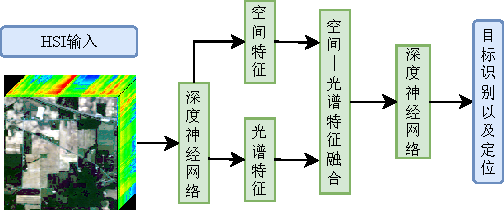
\includegraphics[width=0.74\linewidth]{高光谱目标检测流程.pdf}
    \caption{高光谱目标检测大致流程示意图}
    \label{fig_HTD}
\end{figure}
%%%%%%%%%%%%%%%%%%%%%%%%%%%%%%%%%%%%%%%
相较于传统遥感图像而言,高光谱遥感图像中目标场景更加多样、地物的空间和光谱两大特性更加精细,
因此,通过HSI进行目标检测任务(例如物质勘测、海洋探测等)具有重要意义。
HTD已被广泛应用于监测和实施农业、地质、环境资源评估、城市规划、军事/国防、灾害管理等众多领域 \cite{goetz1985imaging} \cite{teke2013short} \cite{plaza2011parallel}。

从本质上讲,目标检测可以看作是分类和定位的问题 \cite{nasrabadi2013hyperspectral} \cite{zhu2019binary}。
目标检测算法首先通过将目标场景中感兴趣目标的光谱信息和空间信息进行融合,
然后基于融合信息将HSI划分为背景和目标两大类别,最后通过各种现有的检测算法进行识别与定位。
图 \ref{fig_HTD} 展示了高光谱目标检测任务场景的大致流程,其核心步骤主要包括以下三步:

1)利用深度学习技术提取高光谱图像中高级别层次的光谱、空间特征信息;

2)将提取到的空间特征信息和光谱特征信息进行融合;

3)采用Fast R-CNN、YOLO等现有目标检测算法进行识别与定位。


\subsection{相关网络模型介绍}
本小节将介绍本文实验中涉及到的网络模型,主要包括对抗自编码网络(Adversarial Autoendoer,AAE)、VGGNet、ResNet等。

\textbf{AAE}:
2015年Makhzani等人 \cite{makhzani2015adversarial}将先验分布与AE隐空间相结合,并在AE和判别器的基础之上提出了AAE网络,具体网络结构如图 \ref{fig_AAE-Architecture} 所示。
在该图中,上面一行为AE网络模型,
$q\left( \mathbf{z}|\mathbf{x} \right)$表示编码器网络模型,负责对输入数据进行学习、重构,
$p\left( \mathbf{x}|\mathbf{z} \right)$表示解码器网络模型,
$\mathbf{x}$和$\mathbf{\hat{x}}$分别表示编码器的输入数据和解码器的重构结果,
$\mathbf{z}$表示AE网络模型隐空间的输出结果。
该图中下面一行的网络模型被称为判别器,负责区分输入样本是预设的概率分布还是AE网络的隐空间输出,
$p\left(\mathbf{z}\right)$表示概率分布。
AE网络模型隐空间的后验分布表示如下:
%%%%%%%%%%%%%%%%%%%%%%%%%%%%%%%%%%%%%%%
\begin{equation}
    q\left(\mathbf{z}\right) = 
        \int_{x} q\left(\mathbf{z}|\mathbf{x}\right) p_{d}\left(\mathbf{x}\right)dx 
\end{equation}
%%%%%%%%%%%%%%%%%%%%%%%%%%%%%%%%%%%%%%%
生成器的目标是生成分布相似高质量数据,以欺骗判别器,而判别器的目标则是准确地区分生成的数据和真实的数据。
与传统GAN网络模型相比,AAE网络不仅表现更加稳定可靠,而且可以生成与训练数据分布相似的高质量重构数据,常用于图像生成、数据增强、目标检测等各种任务。
%%%%%%%%%%%%%%%%%%%%%%%%%%%%%%%%%%%%%%%
\begin{figure}[ht]
    \centering
    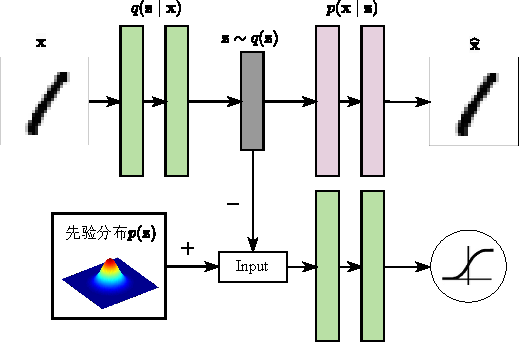
\includegraphics[width=0.8\linewidth]{AAE-Architecture.pdf}
    \caption{对抗自编码网络结构示意图 \cite{makhzani2015adversarial}}
    \label{fig_AAE-Architecture}
\end{figure}
%%%%%%%%%%%%%%%%%%%%%%%%%%%%%%%%%%%%%%%

\textbf{VGGNet}:
VGGNet是一种卷积神经网络模型,设计理念简单,将大量小卷积核($3\times3$)和池化层($2\times2$)堆叠成一个很深的网络结构,例如VGG-16,VGG-19等,
如图 \ref{fig_VGG-ResNet} \subref{fig_VGG} 展示了该类型网络的核心结构。
其中,VGG-16包含16个卷积层和3个全连接层,是最受欢迎的一个网络模型变体。
本文在自然图像分类场景下,会将提出的梯度压缩算法应用于该网络进行算法验证。

%%%%%%%%%%%%%%%%%%%%%%%%%%%%%%%%%%%%%%%
\begin{figure}[t]
    \centering
    \subfloat[VGGNet]{
        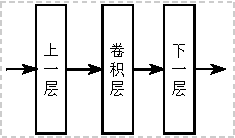
\includegraphics[width=0.3\linewidth]{VGG-Resnet-Inception_1.pdf}
        \label{fig_VGG}
        }
    \subfloat[ResNet]{
        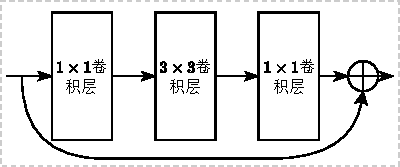
\includegraphics[width=0.42\linewidth]{VGG-Resnet-Inception_2.pdf}
        \label{fig_ResNet}
        }
    \caption{VGGNet和ResNet网络模型核心结构示意图}
    \label{fig_VGG-ResNet}
\end{figure}
%%%%%%%%%%%%%%%%%%%%%%%%%%%%%%%%%%%%%%%

\textbf{ResNet}:
ResNet是一种残差块堆叠而成的深度神经网络,它的设计思想在于引入残差块,
如图 \ref{fig_VGG-ResNet} \subref{fig_ResNet} 所示。
一个残差块包含多个卷积层以及一个恒等映射,将输入数据与卷积层的输出数据进行相加,从而帮助网络模型学习残差信息,解决了深度神经网络训练时梯度消失或爆炸的问题。
相较于VGGNet,该网络模型通常更深,具有更好的泛化能力,计算效率高的优点,
但也具有计算量大、模型参数多等劣势。
本文将在ResNet-56以及ResNet-110两个不同大小的网络模型上验证所提出的梯度压缩算法。

\section{实验数据集与评价指标}
\subsection{实验数据集}
\textbf{AeroRIT} \cite{rangnekar2020aerorit}:
AeroRIT数据集是由罗彻斯特理工学院大学校园上空的塞斯纳飞机上的两种摄像系统采集得到,
第一个采集系统是工作在RGB域的80 magepixel(MP)的框架型硅传感器,
第二个采集系统使用的是可见红外(VNIR)高光谱Headwal Photonics Micro Hyperspec E系列CMOS传感器。
该数据集中的图像数据包含372个波段,波长范围从397 nm到1003 nm,空间尺寸分辨率为$1973\times3975$,包含了将近700万个注释数据,却只被划分为5个类别。

由于该数据集的空间分布不规则,我们进行了适当的切割处理,
即选取位于原始图像的某块矩形图像作为训练数据集,该矩形区域的对于应原始图像左上角和右下角的坐标分别为$(401, 101)$和$(1600, 3900)$。
因此,在评估实验中,对所有波段的图像数据来说,其裁切后的实际有效空间分辨率为$1200\times3800$,高光谱目标和背景分别占用48.67Mb和3196.13Mb内存空间,
如表 \ref{tab_HSI-Water} 描述了验证高光谱目标检测实验中的目标和背景的像素、占比等总体分布情况。
如图 \ref{fig_Result-AeroRIT} \subref{fig_Result-AeroRIT-pseudo-color} 
以及图 \ref{fig_Result-AeroRIT} \subref{fig_Result-AeroRIT-ground-truth} 
两幅子图所示,分别展示了该数据集的伪彩图和目标真实标签的分布状况。

%%%%%%%%%%%%%%%%%%%%%%%%%%%%%%%%%%%%%%%
\renewcommand{\arraystretch}{1.3}
\begin{table*}[ht]
    \centering
    % \caption{ Xiongan New Area(Matiwan Village) 和 AeroRIT 高光谱遥感数据集的目标以及背景的样本数量和空间占比}
    \caption{ Xiongan 和 AeroRIT HSI中目标和背景的样本数量以及空间占比}
    \label{tab_HSI-Water}
    \begin{tabular}{cccc}
        \toprule
        \toprule
            数据集 & 类别 & 样本数量 & 占比($\%$)\\
        \midrule
            \multirow{2}{*}{Xiongan New Area(Matiwan Village)} & 水 & 165647 & 2.80 \\
             & 背景 & 5759353 & 97.20 \\
        \toprule
            \multirow{2}{*}{AeroRIT} & 水 & 68576 & 1.50 \\
            & 背景 & 4491424 & 98.50 \\
        \bottomrule
        \bottomrule
    \end{tabular}
\end{table*}
%%%%%%%%%%%%%%%%%%%%%%%%%%%%%%%%%%%%%%%

\textbf{Xiongan New Area(Matiwan Village)} \cite{yi2020aerial}:
2017年10月,该航空高光谱遥感图像采用中国科学院技术物理研究所设计的可见光及近红外成像光谱仪拍摄。
该数据集有256个波段,波长范围为400至1000nm,空间分辨率为$3750\times1580$,包含19种土地覆盖类别。
在本文的验证实验中,“水”将被视为感兴趣的高光谱目标,而其他类别被视为背景样本,
分别占用近0.896GB和31.104GB的内存空间,具体的像素数量及其空间占比如表 \ref{tab_HSI-Water} 所示。
如图 \ref{fig_Result-Xiongan} \subref{fig_Result-Xiongan-pseudo-color} 
以及图 \ref{fig_Result-Xiongan} \subref{fig_Result-Xiongan-ground-truth} 
两幅子图所示,分别展示了该数据集的伪彩图和目标真实标签的分布状况。
为了简化后续图表标题,“Xiongan New Aera(Matiwan Village)”将被简化为“Xiongan”。

\textbf{CIFAR10}:
该数据数据集包含10种具有标签的图片集合,它们相互独立、互不重叠。
每一种类型的图片包括5000张训练样本以及1000张测试样本,每张图片大小为$32\times32$,如图 \ref{fig_CIFAR10_image} 展示了类别标签和一些图片样张。
在本论文的自然图像分类实验中,我们将首先使用图片增强技术对该数据集进行简单预处理,然后再将预处理后的图像作为训练数据。

%%%%%%%%%%%%%%%%%%%%%%%%%%%%%%%%%%%%%%%
\begin{figure}[ht]
    \centering
    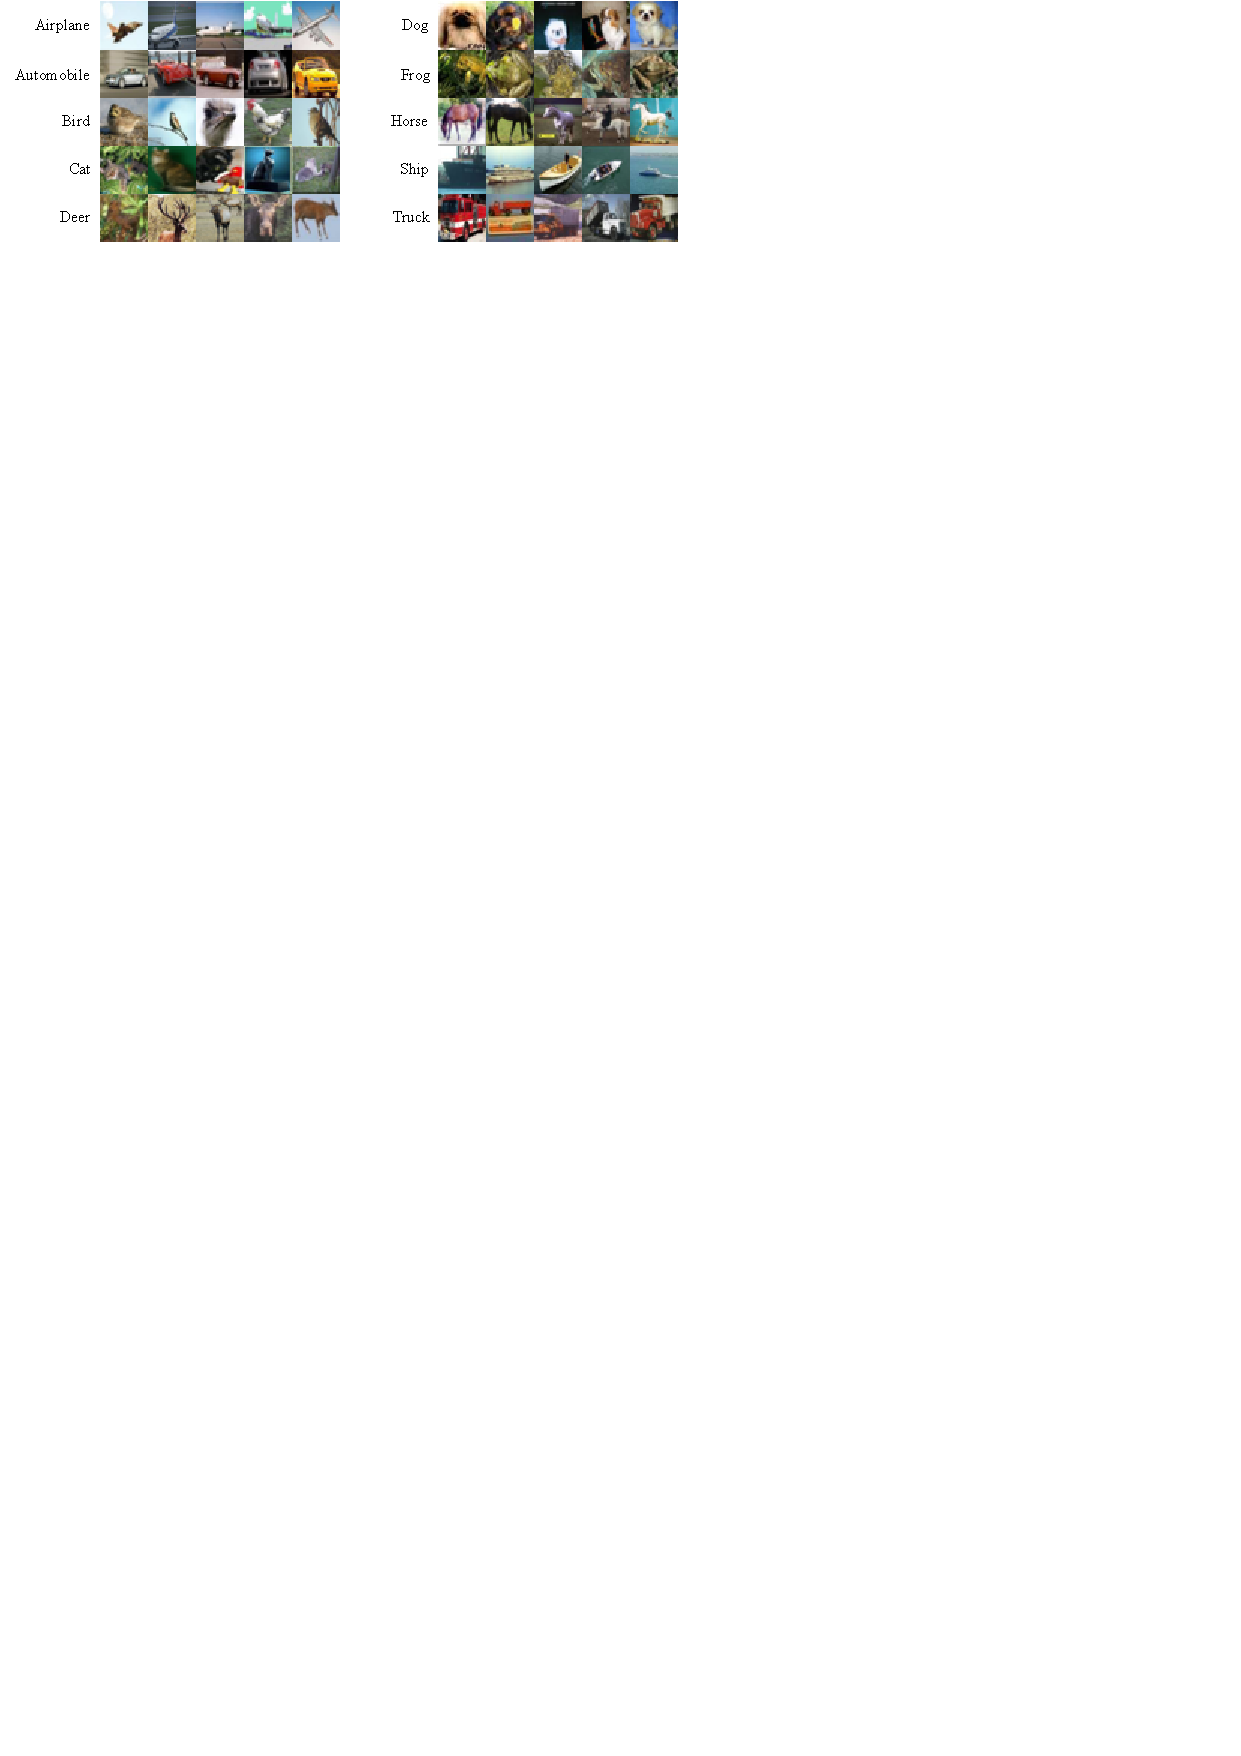
\includegraphics[width=0.98\textwidth]{CIFAR10_image-v2.pdf}
    \caption{CIFAR10数据集标签及其部分图片样张}
    \label{fig_CIFAR10_image}
\end{figure}
%%%%%%%%%%%%%%%%%%%%%%%%%%%%%%%%%%%%%%%

\subsection{评价指标}
在目标检测领域,从评价个体的角度可以将性能指标分以下两种:主观评价、客观评价。
主观评价,通常指的是人们基于实验结果,采用视觉与直观感受进行评价的一种评价指标,但评价结果会受到较强的主观因素的影响。
客观评价,通常指的是采用某种量化数据对实验结果进行客观分析,可以很好的避免主观因素介入,应用更为广泛。
本文将根据不同的下游任务进行不同性能评价指标的选择。
例如,高光谱目标检测任务采用主观评价和客观评价,而自然图像分类任务将仅采用客观评价。
接下来,本小节将对本文中涉及到到的评价指标进行阐述。

ROC(Receiver Operating Characteristic)曲线 \cite{swets2000better}:
它是一种检测器性能的二维评价指标,是一条关于检测器的检测率和误报率的曲线。
但为了通过单个标量来表示检测器的性能,通常采取的措施是计算ROC曲线下的面积,被称为AUC\cite{bradley1997use},如公式 \eqref{eq_AUC_FPR} 所示。
%%%%%%%%%%%%%%%%%%%%%%%%%%%%%%%%%%%%%%%
\begin{equation}
    \begin{aligned}
        F_{0}\left(\tau\right) &= \frac{TP\left(\tau\right)}{TP\left(\tau\right)+FN\left(\tau\right)} \\
        F_{1}\left(\tau\right) &= \frac{TP\left(\tau\right)}{TN\left(\tau\right)+FP\left(\tau\right)}
    \end{aligned}
\end{equation}
%%%%%%%%%%%%%%%%%%%%%%%%%%%%%%%%%%%%%%%
其中,$\tau$表示给定的分割阈值,并定义分数大于等于分割阈值的像素为正样本,
$F_{0}\left(\tau\right)$表示检测率,$F_{1}\left(\tau\right)$表示虚警率,
给定阈值$\tau$时,
$TP\left(\tau\right)$表示被预测为正样本的目标像素数量,
$FN\left(\tau\right)$表示被预测为负样本的目标像素数量,
$FP\left(\tau\right)$表示被预测为正样本的背景像素数量,
$TN\left(\tau\right)$表示被预测为负样本的背景像素数量。
虚警率(False Positive Rate,FPR)以及AUC计算公式 \eqref{eq_AUC_FPR} 如下:
%%%%%%%%%%%%%%%%%%%%%%%%%%%%%%%%%%%%%%%
\begin{equation}
    \begin{aligned}
        FPR &= \int_{0}^{1} F_{1}(s)ds \\
        AUC &= \int_{0}^{1} F_{0}(s)dF_{1}(s)
    \end{aligned}
    \label{eq_AUC_FPR}
\end{equation}
%%%%%%%%%%%%%%%%%%%%%%%%%%%%%%%%%%%%%%%

在本文高光谱目标检测任务场景中,将采用AUC和FPR作为其客观评价指标,
AUC$\left(F_{0}(\tau), F_{1}(\tau)\right)$的值越大表示检测精度越高,
AUC$\left(F_{1}(\tau), F_{0}(\tau)\right)$的值越小表示虚警率越低。

本文自然图像分类任务任务场景中,将采用Top-k分类精度($acc_{k}$)作为客观评价指标,$k$通常设为${\{1, 5\}}$,具体来说,其计算公式 \eqref{eq_Top-k} 如下:
%%%%%%%%%%%%%%%%%%%%%%%%%%%%%%%%%%%%%%%
\begin{equation}
    acc_{k} = \frac{N_{C^{k}}}{N_{C^{T}}}
    \label{eq_Top-k}
\end{equation}
%%%%%%%%%%%%%%%%%%%%%%%%%%%%%%%%%%%%%%%
其中,$N_{C^{k}}$表示所有测试结果中前$k$类标签中正确的预测数量,$N_{C^{T}}$表示所有测试图像的标签数量。

除了以上常用的评价指标之外,梯度压缩算法的复杂度、鲁棒性等性能指标也可作为目标检测任务、分类任务的参考指标。

\section{本章小结}
本章主要针对深度学习技术、分布式训练、高光谱目标检测任务、图像分类任务等涉及到的知识进行介绍。
首先介绍了深度学习的相关基础理论知识,紧接着介绍了分布式训练相关的理论基础,并指出了目前大数据大模型场景下引入分布式训练的必要性,
然后阐述了分布式训练中的并行方式、拓扑架构、同步方式等必要组件,同时对现有分布式平台进行简单介绍,并选择使用Horovod作为本论文实验的部署平台。
接下来,介绍了高光谱目标检测以及图像分类的相关知识,包括检测流程以及相关网络模型。
最后,对本文下游任务的相关实验数据集与评价指标进行阐述。


%%%%%%%%%%%%%%%%%%%%%%%%%%%%%%%%%%%%%%%%%%%%%%%%%%%%%%%%%%%
%%%%%%%%%%%%%%%%%%%%%%%%%%%%%%%%%%%%%%%%%%%%%%%%%%%%%%%%%%%
\chapter{基于近似质心的梯度压缩算法}
\label{sec_chapter-3}
\section{引言}
本章首先根据第\ref{sec_chapter-2}章相关理论基础,发现并指出了目前分布式训练的技术难点,
即高频的、全尺寸全精度数据格式的网络通信行为可能导致分布式训练速度慢,甚至无法在短时间内顺利完成训练。
为了解决该技术难题,本章提出了基于近似质心的梯度压缩算法(Gradient Compression via Approximate Centroid,GCAC),
该算法根据网络模型每一层的梯度分布状况选择接近质心的梯度进行优选,降低了不同Worker之间网络通信的数据量,并采用Horovod + PyTorch网络框架搭建分布式平台进行实现和验证。

本章第 \ref{sec_GCC} 节详细介绍提出的基于近似质心的梯度压缩算法;
第 \ref{sec_ResultAndAnalisy} 节对提出的基于近似质心的梯度压缩算法进行实验验证,主要包括高光谱目标检测和图像分类两大任务场景,并对实验结果进行分析;
第 \ref{sec_Summary-3} 节对本章的研究工作进行总结。

\section{基于近似质心的梯度压缩算法}
\label{sec_GCC}
\subsection{网络模型中局部梯度分析}
\label{sec_LocalGradient}
在分布式训练过程中,虽然Allreduce算法优化加速了各Worker之间的梯度同步,但是待传输梯度数据量过大仍然可能导致通信瓶颈问题。
为了减少分布式训练的通信开销并最大化利用分布式集群中各个Worker的利用率,我们将梯度压缩算法应用于分布式训练技术。
同时,本节对梯度特征进行了实验性分析,以更好地实施梯度压缩算法。

目前,大多数梯度压缩算法以梯度值或范数大小作为重要性度量,通常需要满足以下两个隐含条件才能取得比较不错的效果:

1)梯度值或范数越小,对模型优化贡献越小;

2)梯度值或范数的标准差足够大。

然而,在实际训练过程中,上述提及的两个隐含条件不总是成立。因此,我们抓取并分析了局部梯度之间的冗余相关性,以便更好地裁剪冗余梯度。
如图 \ref{fig_Gradient-Distribution-1} (a) 展示了压缩前的梯度分布状况,可以看到,绝大多数梯度值较小且接近于0。
当采用基于梯度值的梯度压缩算法且压缩比设置为2时,压缩后的梯度分布状况如图 \ref{fig_Gradient-Distribution-1} (b) 所示,
其中位于设定阈值线(红色点状线)之间的梯度将被重置为0,并且不会参与网络各Worker之间的网络通信。
需要注意的是,当采用这种重要性度量时,梯度值或范数越大,通常该梯度对网络模型参数优化的贡献越大;
但度量相对较小的梯度无法被证明其重要性小,因为度量较小不一定是因为其梯度值或范数小,
也可能是因为在分布式训练的一次迭代中所有梯度的值或范数都比较大。
在这种情况下,裁剪掉梯度值或范数小的梯度无疑将严重影响网络模型的性能表现。
另外,当局部梯度值或范数的标准差很小时,以压缩比为目标去选择一个合适的分割阈值通常是困难的。
一旦选择的阈值不合适,大量梯度关键信息将会被裁剪,同样会导致网络模型性能下降严重。

%%%%%%%%%%%%%%%%%%%%%%%%%%%%%%%%%%%%%%%
\begin{figure}[t]
    \centering
    \subfloat[压缩前梯度分布]{
        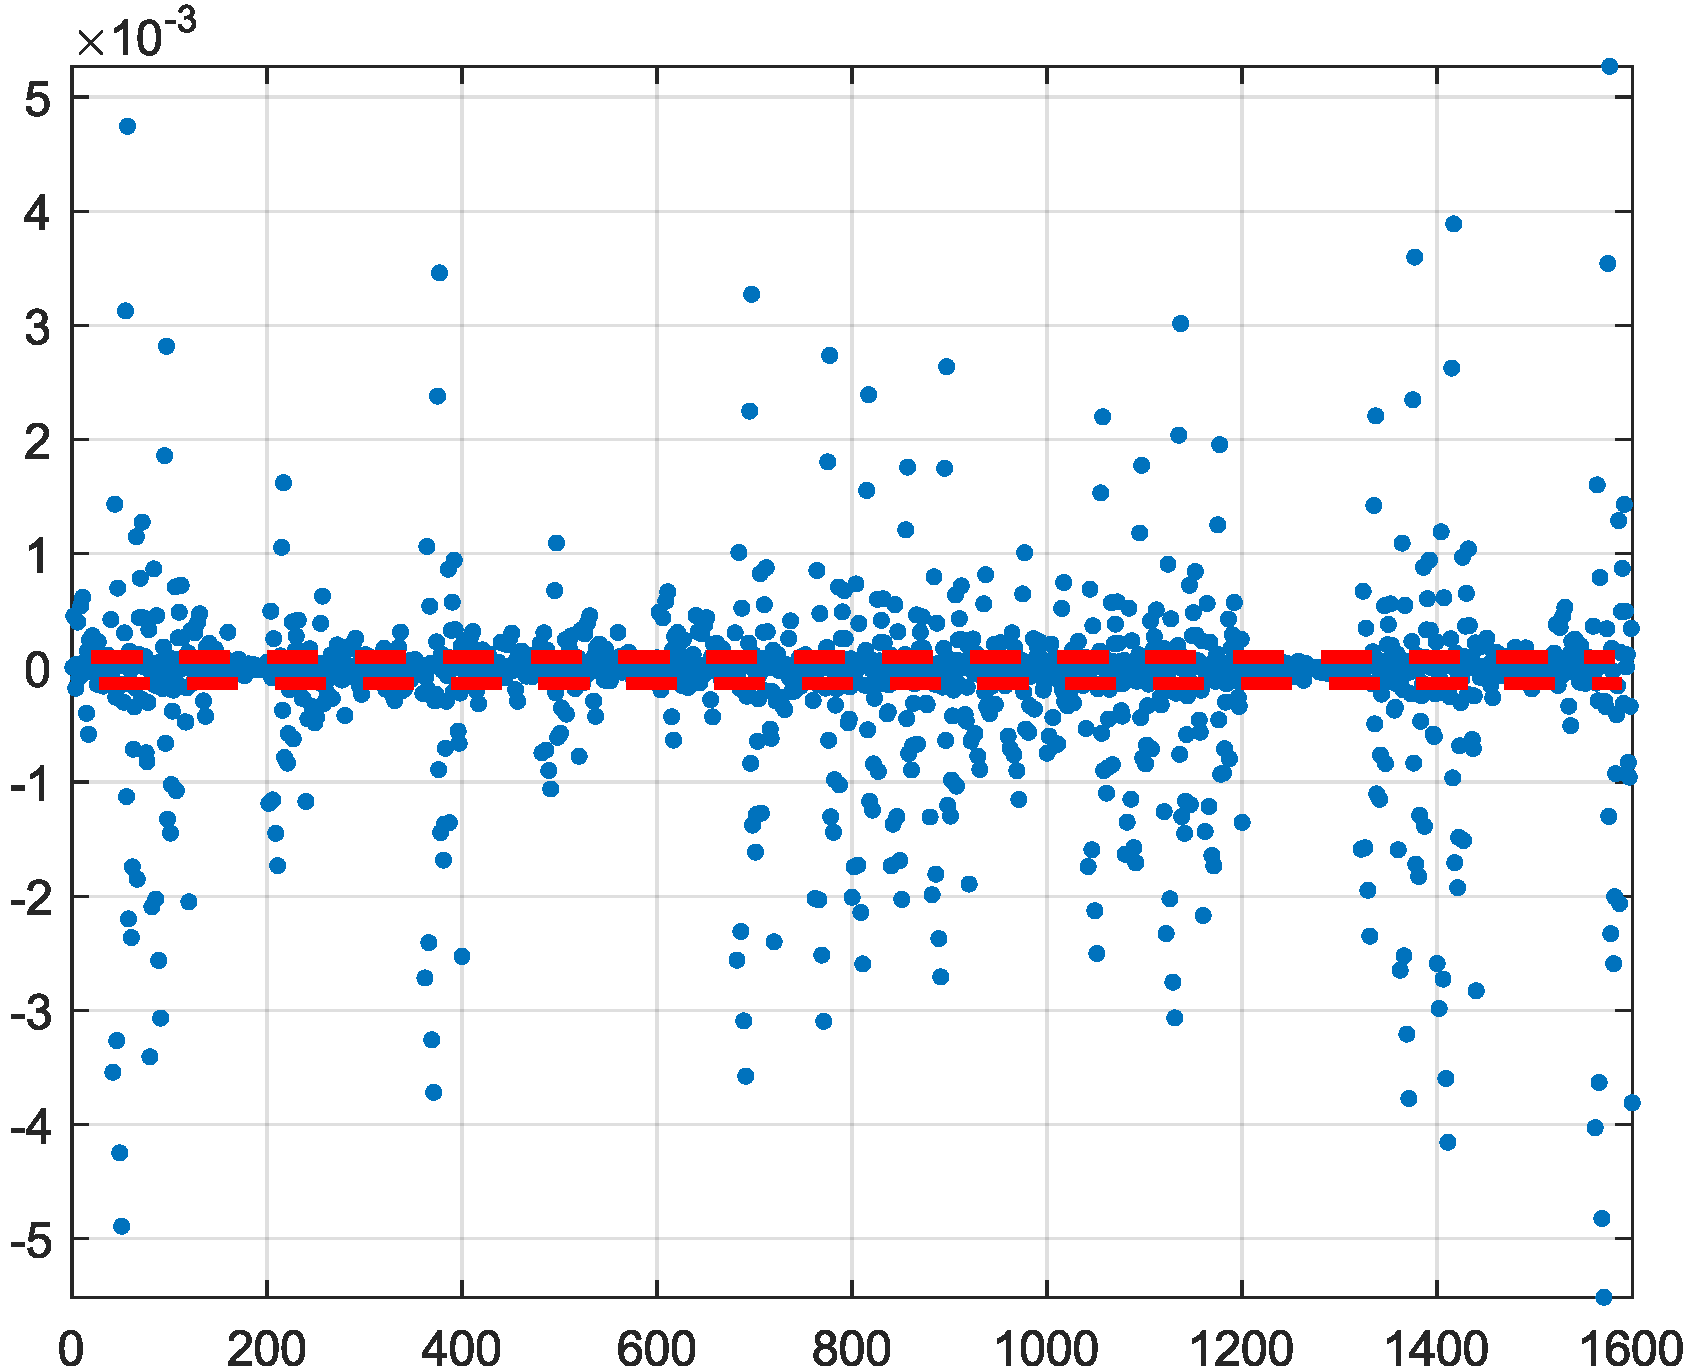
\includegraphics[width=0.47\linewidth]{gradient-0.pdf}
        \label{fig_Gradient-Distribution-Before-Compression}
    }
    \subfloat[压缩后梯度分布]{
        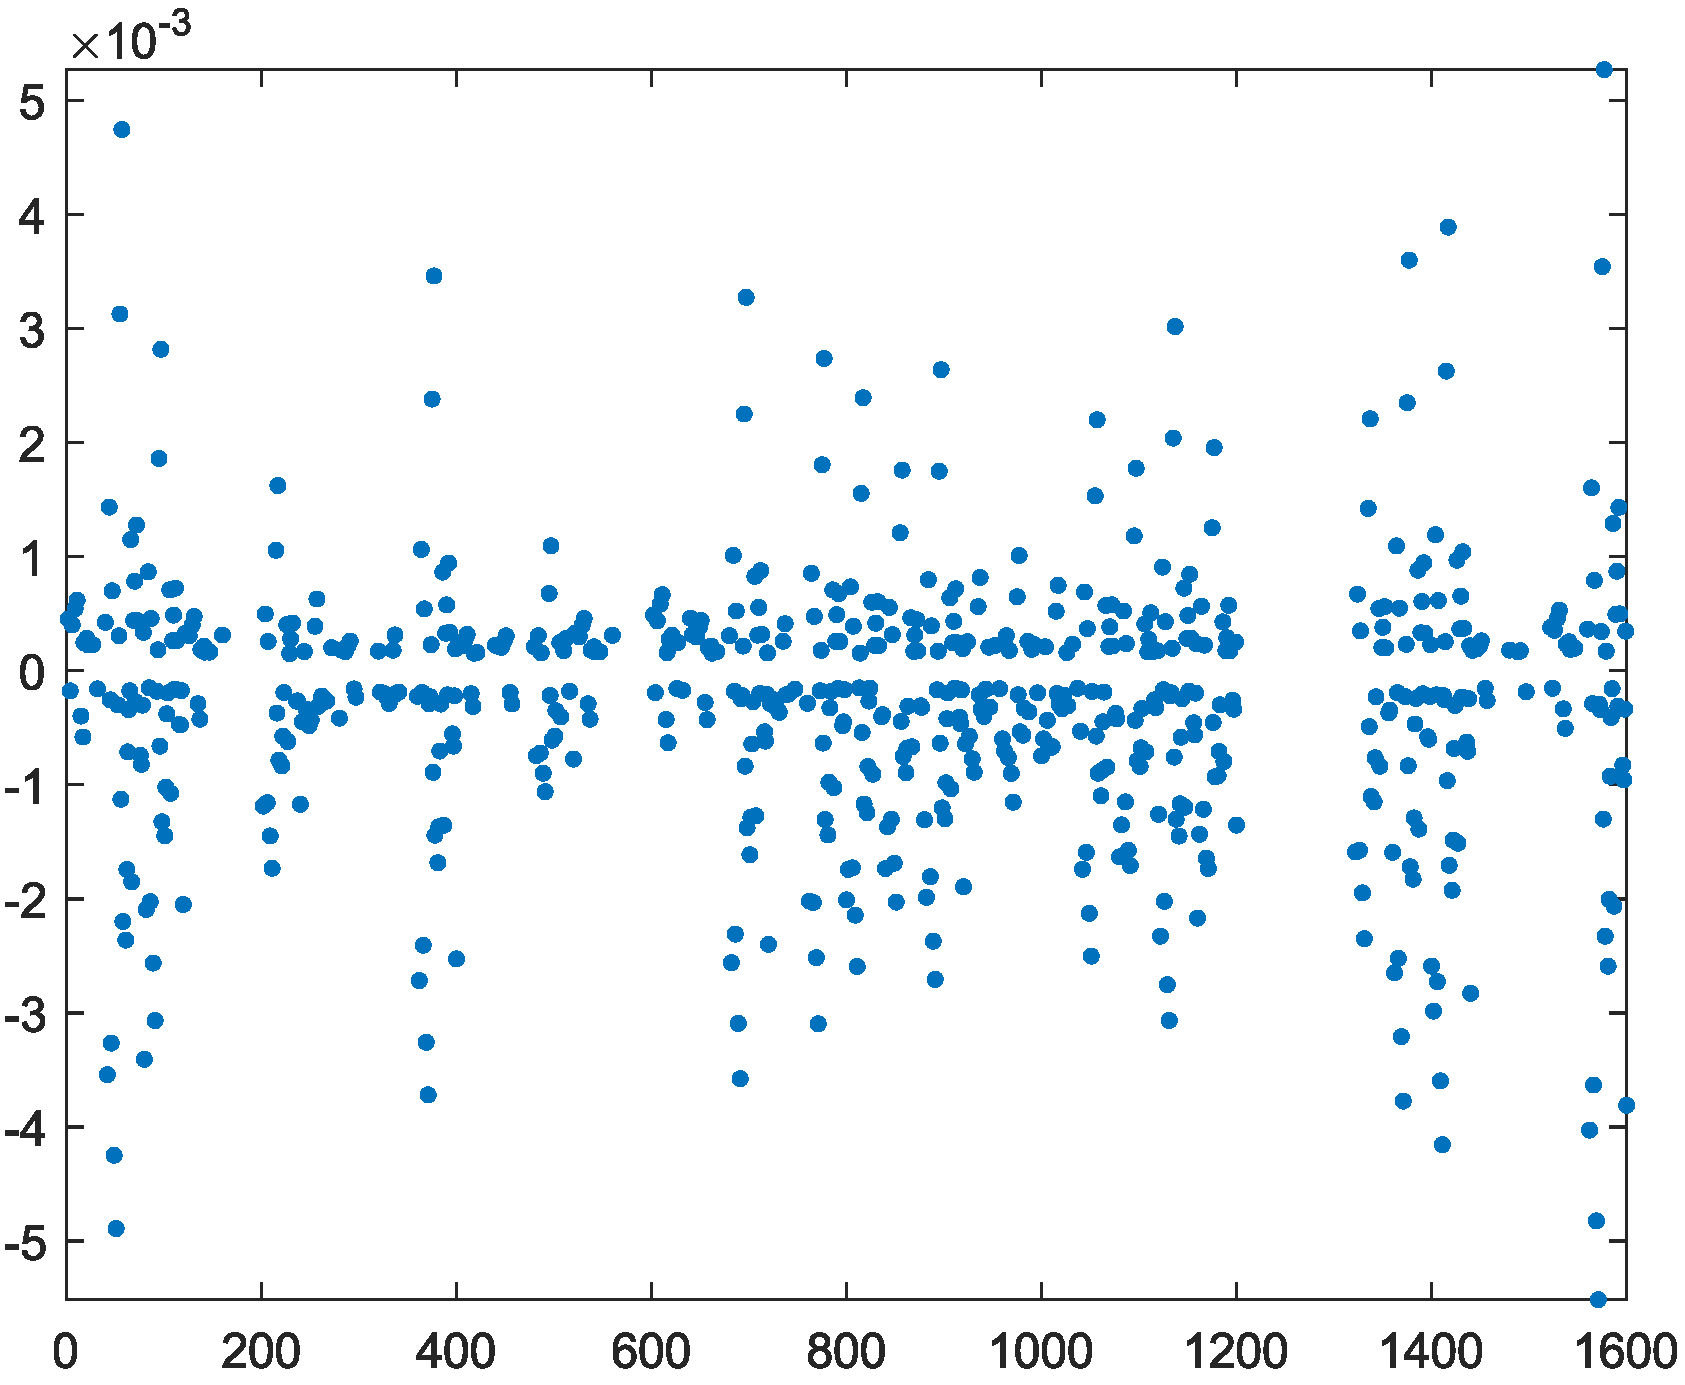
\includegraphics[width=0.47\linewidth]{gradient-1.pdf}
        \label{fig_Gradient-Distribution-After-Compression}
    }
    \caption{网络模型采用传统方法压缩前后的梯度分布}
    \label{fig_Gradient-Distribution-1}
\end{figure}
%%%%%%%%%%%%%%%%%%%%%%%%%%%%%%%%%%%%%%%

基于以上分析可知,仅仅依赖梯度值或范数大小就决定某个梯度是否重要存在不可靠的情况。
因此,我们在受到Fletcher等人\cite{fletcher2008robust}的启发,
基于Euclidean空间中的质心揭示共同属性的假设,即质心等效于局部梯度张量的中心或公共属性,
将梯度映射到Euclidean空间并计算梯度张量的质心,
并通过分析Euclidean空间中的点进一步揭示各个梯度之间的冗余关系,
提出一种基于质心的重要性度量方法,克服了传统方法不总满足的依赖条件。

%%%%%%%%%%%%%%%%%%%%%%%%%%%%%%%%%%%%%%%
\begin{figure}[ht]
    \centering
    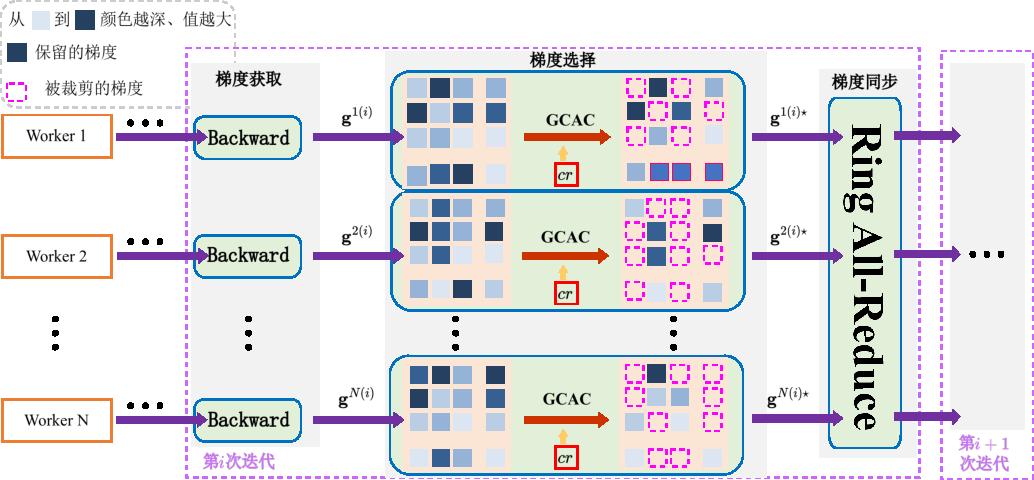
\includegraphics[width=0.884\textwidth]{GCC-Outline.pdf}
    \caption{基于近似质心的梯度压缩算法应用框图}
    \label{fig_GCC-Outline}
\end{figure}
%%%%%%%%%%%%%%%%%%%%%%%%%%%%%%%%%%%%%%%
\subsection{基于近似质心的梯度压缩算法}
为了避免 \ref{sec_LocalGradient} 小节所讨论的梯度值或范数依赖条件问题,
本小节将介绍我们提出基于近似质心的梯度压缩算法。
GCAC算法的核心思想是从信息冗余的角度出发,替换掉那些可被代替的梯度。
如图 \ref{fig_GCC-Outline} 为GCAC算法的应用框图,展示了GCAC算法如何在分布式训练过程中发挥作用。

第$m$个Worker上网络模型的第$k$层梯度$\mathbf{g}^{m[k]}\in \mathbb{R}^{\left(n^{m[k]}+1 \right) \times Q^{m[k]}}$构成的梯度矩阵如公式 \eqref{eq_Gradient-matrix} 所示:
%%%%%%%%%%%%%%%%%%%%%%%%%%%%%%%%%%%%%%%
\begin{equation}
  \mathbf{g}^{m[k]} =
  \begin{bmatrix}
          g^{m[k]}_{0, 0} & \dots  &  g^{m[k]}_{0, Q^{m[k]}} \\
          \vdots        & \ddots & \vdots \\
          g^{m[k]}_{n^{m[k]}, 0} & \dots  & g^{m[k]}_{n^{m[k]}, Q^{m[k]}} \\
  \end{bmatrix}%_{Q^{m[k]} \times R^{m[k]}}   % 矩阵下标
  \label{eq_Gradient-matrix}
\end{equation}
%%%%%%%%%%%%%%%%%%%%%%%%%%%%%%%%%%%%%%%
其中,$Q^{m[k]}$表示$m$节点中第$k$层中神经元梯度的尺寸。
局部梯度矩阵的质心$\mathcal{C}^{m[k]}$可通过计算公式 \eqref{eq_Gradient-Centroid} 求得:
%%%%%%%%%%%%%%%%%%%%%%%%%%%%%%%%%%%%%%%
\begin{equation}
    \begin{aligned}
        \psi \left(\mathcal{C}\right) & \triangleq
            \sum_{i = 0}^{n^{m[k]}} \sum_{j = 0}^{Q^{m[k]}}
                \left\lVert \mathcal{C} - g_{i,j}^{m[k]} \right\rVert_{2}, \\
        \mathcal{C}^{m[k]} &=
            \arg \min_{\mathcal{C}\in \mathbb{R}^{d}}\psi\left(\mathcal{C}\right)
        % \mathcal{C}^{m[k]} = \arg \min_{\mathcal{C}\in \mathbb{R}^{d}}
        %     \sum_{i = 0}^{n^{m[k]}} \sum_{j = 0}^{Q^{m[k]}}
        %         {\left\lVert \mathcal{C} - g_{i,j}^{m[k]} \right\rVert}_{2}
    \end{aligned}
    \label{eq_Gradient-Centroid}
\end{equation}
%%%%%%%%%%%%%%%%%%%%%%%%%%%%%%%%%%%%%%%
基于已获得的质心,可通过公式 \eqref{eq_Gradient-Closed2-Centroid} 获取最接近质心的梯度$\mathbf{g}_{i^{\star}, j^{\star}}^{m[k]}$:
%%%%%%%%%%%%%%%%%%%%%%%%%%%%%%%%%%%%%%%
\begin{equation}
    \begin{aligned}
        \mathbf{g}_{i^{\star}, j^{\star}}^{m[k]} & =
            \mathop{\arg\min}\limits_{g_{i', j'} \in \mathbb{R}^{d}}
                {\left\lVert \mathbf{g}_{i', j'}^{m[k]} - \mathcal{C}^{m[k]} \right\rVert}_2, \\
        & s.t. i'\in \left\{0, 1, \dots, Q^{m[k]}\right\}, j'\in \left\{0, 1, \cdots, Q^{m[k]} \right\}
    \end{aligned}
    \label{eq_Gradient-Closed2-Centroid}
\end{equation}
%%%%%%%%%%%%%%%%%%%%%%%%%%%%%%%%%%%%%%%
根据质心相关特性可知,$\mathbf{g}_{i^{\star}, j^{\star}}^{m[k]}$可被本层网络模型中其他梯度线性表示,
裁剪掉这些接近质心的冗余梯度并不会对网络模型参数优化产生太大的影响。
值得注意的是,通过深入分析公式 \eqref{eq_Gradient-Centroid} 
以及公式 \eqref{eq_Gradient-Closed2-Centroid},可得出以下两个结论:

1)\textbf{通过公式 \eqref{eq_Gradient-Centroid} 求解局部梯度质心是极其耗时的}:由于梯度矩阵中各梯度不满足均匀分布的特性,则需要进行遍历求解,时间复杂度为$O\left(n^{m[k]} \times Q^{m[k]}  \right)$;

2)\textbf{接近质心的待裁剪梯度候选者$\mathbf{g}_{i^{\star}, j^{\star}}^{m[k]}$来源于本层梯度矩阵}:
基于公式 \eqref{eq_Gradient-Centroid} 得到的质心$\mathcal{C}^{m[k]}$,
采用公式 \eqref{eq_Gradient-Closed2-Centroid} 进行梯度选择得到梯度候选者,
且满足$\mathbf{g}_{i^{\star}, j^{\star}}^{m[k]} \in \mathbf{g}^{m[k]}$。

因此,为了解决结论1)的梯度计算耗时问题,我们在充分利用结论2)的基础上,提出了一个求解该问题的加速计算技术。
该加速计算算法是一个计算更方便、耗时更短的近似公式,其主要核心思想是最小化梯度候选者与其他梯度之间的距离之和,如公式 \eqref{eq_Gradient-equivalent-formula} 所示,
其中,$\mathbf{g}_{i^{\star}, j^{\star}}^{m[k]}$将作为本层梯度质心的近似替代者,称为“近似质心”,并在之后的计算中代替局部梯度质心的作用。
为了方便后续描述,将$\mathbf{g}_{i^{\star}, j^{\star}}^{m[k]}$简记为$\hat{\mathcal{C}}^{m[k]}$。
%%%%%%%%%%%%%%%%%%%%%%%%%%%%%%%%%%%%%%%
\begin{equation}
    \begin{aligned}
        &\mathbf{g}_{i^{\star}, j^{\star}}^{m[k]} =
            \mathop{\arg\min}\limits_{\mu} 
                \sum_{i'=0}^{n^{m[k]}} \sum_{j'=0}^{Q^{m[k]}}
                    \left\lVert 
                        g_{i', j'}^{m[k]} - \mathbf{\mu} 
                    \right\rVert_{2}, \\
        s.t. \ &\left|g_{i', j'}^{m[k]} - \mathbf{\mu}\right|>0,
        \ \mu \in \left\{ g_{0, 0}^{n[k]}, \dots, g_{Q^{m[k]}, Q^{m[k]}}^{m[k]} \right\}
    \end{aligned}
    \label{eq_Gradient-equivalent-formula}
\end{equation}
%%%%%%%%%%%%%%%%%%%%%%%%%%%%%%%%%%%%%%%

质心在Euclidean空间中是经典的数据中心估计器\cite{fletcher2008robust},被选中的近似质心$\hat{\mathcal{C}}^{m[k]}$和剩下的梯度共享某些共同属性。
换句话说,质心等效于局部梯度矩阵的中心或公共属性,然后将其余梯度视为一组基向量,
这组基向量可以将接近质心的梯度$\hat{\mathcal{C}}^{m[k]}$完备地线性表示,
也可以引导模型朝着最优的梯度下降方向进行优化。
% 裁剪掉接近质心的梯度对模型参数的优化将不会产生较大的影响。

另外,为了满足梯度压缩多样性的要求,必须对局部梯度进行排序操作。
在根据公式 \eqref{eq_Gradient-equivalent-formula} 求得最接近质心的梯度候选者$\hat{\mathcal{C}}^{m[k]}$后,
然后通过公式 \eqref{eq_Gradient-rank-formula} 进行计算“近似质心”与其他梯度之间的距离$s$(本文采用欧几里得范数作为距离度量):
%%%%%%%%%%%%%%%%%%%%%%%%%%%%%%%%%%%%%%%
\begin{equation}
    \begin{aligned}
        s_{j'}^{m[k]} &\triangleq \phi\left(\hat{\mathcal{C}}^{m[k]}, g_{i, j}^{m[k]} \right) =
            \left\lVert \hat{\mathcal{C}}^{m[k]} - g_{i, j}^{m[k]} \right\rVert_2, \\
        s.t. \ \Lambda^{m[k]} \triangleq
            n^{m[k]} \times & Q^{m[k]},
        \quad i \in \left[ 0, n^{m[k]} \right],
        \quad j \in \left[ 0, Q^{m[k]} \right],
        \quad j'\in\left[1, \Lambda^{m[k]} \right] \\
    \end{aligned}
    \label{eq_Gradient-rank-formula}
\end{equation}
%%%%%%%%%%%%%%%%%%%%%%%%%%%%%%%%%%%%%%%
并定义梯度距离和列表$\mathcal{S}\in \mathbb{R}^{\Lambda^{m[k]}}$,如公式 \eqref{eq_Gradient-sum} 所示:
%%%%%%%%%%%%%%%%%%%%%%%%%%%%%%%%%%%%%%%
\begin{equation}
    \mathcal{S}^{m[k]} \triangleq 
        \left\{ 
            s_{1}^{n[k]}, \dots, s_{\Lambda^{n[k]}}^{n[k]} 
        \right\}
    \label{eq_Gradient-sum}
\end{equation}
%%%%%%%%%%%%%%%%%%%%%%%%%%%%%%%%%%%%%%%
然后将局部的$\mathcal{S}$进行排序(默认采用升序),得到$\mathcal{S}^\star$,如公式 \eqref{eq_Gradient-sum-sort} 所示:
%%%%%%%%%%%%%%%%%%%%%%%%%%%%%%%%%%%%%%%
\begin{equation}
    {\mathcal{S}^{m[k]}}^\star = Sort\left(
            \mathcal{S}^{m[k]}, increase=True
        \right)
    \label{eq_Gradient-sum-sort}
\end{equation}
%%%%%%%%%%%%%%%%%%%%%%%%%%%%%%%%%%%%%%%
最后,根据排序后结果$\mathcal{S}^\star$有选择性地裁剪某些梯度,并在适当时机采用Allreduce通信原语进行网络模型梯度更新:

1)根据给定的梯度压缩条件(目标梯度压缩比$cr$),在$\mathcal{S}^\star$中搜索对应的索引$\kappa$,
使其满足压缩条件,得到保留目标梯度列表$\mathfrak{g}^{n[k]}$,如公式 \eqref{eq_Gradient-sum-search} 所示:
%%%%%%%%%%%%%%%%%%%%%%%%%%%%%%%%%%%%%%%
\begin{equation}
    \begin{aligned}
        \kappa &= Search \left({\mathcal{S}^{m[k]}}^\star, cr\right), \\
       \hat{\mathcal{S}}^{m[k]} &= {\mathcal{S}^{m[k]}}^{\star}\left[\kappa, \Lambda^{m[k]} \right]
            = \left\{
                s_{\kappa}^{m[k]}, s_{\kappa+1}^{m[k]}, \dots, s_{\Lambda^{m[k]}}^{m[k]}
            \right\} ,\\
        & s.t. \min_{\hat{cr} >= cr} \left\lvert \hat{cr} - cr \right\rvert \\
    \end{aligned}
    \label{eq_Gradient-sum-search}
\end{equation}
%%%%%%%%%%%%%%%%%%%%%%%%%%%%%%%%%%%%%%%
其中,$\hat{cr} \in [1, +\infty)$表示实际梯度压缩比,计算公式 \eqref{eq_Gradient-cr-hat} 所示,
$\left\lvert \hat{cr} - cr \right\rvert$表示实际梯度压缩比与目标梯度压缩比两个标量之间绝对值计算操作,然后通过得到的$\hat{\mathcal{S}}^{m[k]}$反向推导出目标梯度处于原始梯度中的位置信息$\mathfrak{g}^{m[k]}$。

%%%%%%%%%%%%%%%%%%%%%%%%%%%%%%%%%%%%%%%
\begin{equation}
    \begin{aligned}
        \hat{cr} &= \frac{\Lambda^{m[k]}}
                    {\sum_{t = 0}^{\Lambda^{m[k]}} \delta\left(
                                        s_{t}^{m[k]}\right)}, \\
        \delta\left(s^{m[k]}\right) &=
        \begin{cases}
            1 & \text{if } s^{m[k]} \in \hat{\mathcal{S}}^{m[k]},\\
            0 & \text{others}.
        \end{cases}
    \end{aligned}
    \label{eq_Gradient-cr-hat}
\end{equation}
%%%%%%%%%%%%%%%%%%%%%%%%%%%%%%%%%%%%%%%

2)网络拓扑中各Worker之间更新神经网络模型梯度、参数,如公式 \eqref{eq_Gradient-update} 所示:
%%%%%%%%%%%%%%%%%%%%%%%%%%%%%%%%%%%%%%%
\begin{equation}
    {\mathbf{g}^{n[k]}}^{\star} = 
        Update\left( \mathbf{g}^{n[k]}, \mathfrak{g}^{n[k]} \right)
    \label{eq_Gradient-update}
\end{equation}
%%%%%%%%%%%%%%%%%%%%%%%%%%%%%%%%%%%%%%%
其中,${\mathbf{g}^{n[k]}}^{\star}$表示更新后的最新网络模型梯度,处于$\mathfrak{g}^{n[k]}$位置的梯度值保持不变的同时其他梯度值被重置为0。
在分布式训练过程中,由于非零梯度保留了重要信息,仍可以用来引导网络模型继续朝着正确方向进行优化,GCAC算法应用于分布式训练的大致流程如算法 \ref{alg_GCC} 所示。

%%%%%%%%%%%%%%%%%%%%%%%%%%%%%%%%%%%%%%%
\renewcommand{\arraystretch}{1.3}
\begin{algorithm}[ht]
    \caption{单节点上GCAC算法整体框架及流程}
    \label{alg_GCC}
    \raggedright
    \hspace*{0.02in} \textbf{输入:}训练数据$X^{n[k]}$,目标梯度压缩比$cr$,最大迭代轮数$Epoch_{max}$,网络模型权重$\mathbf{W}$ \\
    \hspace*{0.02in} \textbf{输出:}训练完成的网络模型权重$\mathbf{\hat{W}}$ \\
    \hspace*{0.02in} \textbf{算法:} 
    \begin{algorithmic}[1]
        \For{$e=1$; $e \leqslant Epoch_{max}$; $e$++}
            \State 获取局部梯度$\mathbf{g}^{n[k]}$
            \For{$k=1$; $k \leqslant n^{[k]}$; $k$++}
                \State 初始化:${\mathcal{S}_{i, j}^{n[k]}}^{\star} \leftarrow \varnothing$
                \State 根据公式 \eqref{eq_Gradient-equivalent-formula} 获取最接近质心的梯度$\mathbf{g}_{i^{\star}, j^{\star}}^{n[k]}$
                \State 根据公式 \eqref{eq_Gradient-rank-formula}、\eqref{eq_Gradient-sum}、\eqref{eq_Gradient-sum-sort} 更新已排序梯度列表${\mathcal{S}_{i, j}^{n[k]}}^{\star}$
                \State 根据公式 \eqref{eq_Gradient-sum-search}、\eqref{eq_Gradient-cr-hat} 搜索满足$cr$的列表索引,并获取$\mathfrak{g}^{n[k]}$
                \State 根据公式 \eqref{eq_Gradient-update},将获取到的$\mathfrak{g}^{n[k]}$置零并更新${\mathbf{g}^{n[k]}}^{\star}$
            \EndFor
            \State 根据设定的Allreduce算法,在合适的时机与其他Worker进行梯度同步
            \State $\mathbf{\hat{W}} \leftarrow \mathbf{W}^{(t+1)} \leftarrow SGD\left( \mathbf{W}^{(t)}, {\mathbf{g}^{n[k]}}^{\star} \right)$
        \EndFor
        \State return $\mathbf{\hat{W}}$
    \end{algorithmic}
\end{algorithm}
%%%%%%%%%%%%%%%%%%%%%%%%%%%%%%%%%%%%%%%

为了更好地展示本章提出的基于近似质心的梯度压缩算法效果,如图 \ref{fig_Gradient-Compression-Distribution-2} 所示,其中,$t$是梯度列表中对应索引。
%%%%%%%%%%%%%%%%%%%%%%%%%%%%%%%%%%%%%%%
\begin{figure}[ht]
    \centering
    % \includegraphics[width=0.7\textwidth]{gradient-2111.pdf}
    \subfloat[压缩前梯度分布]{
        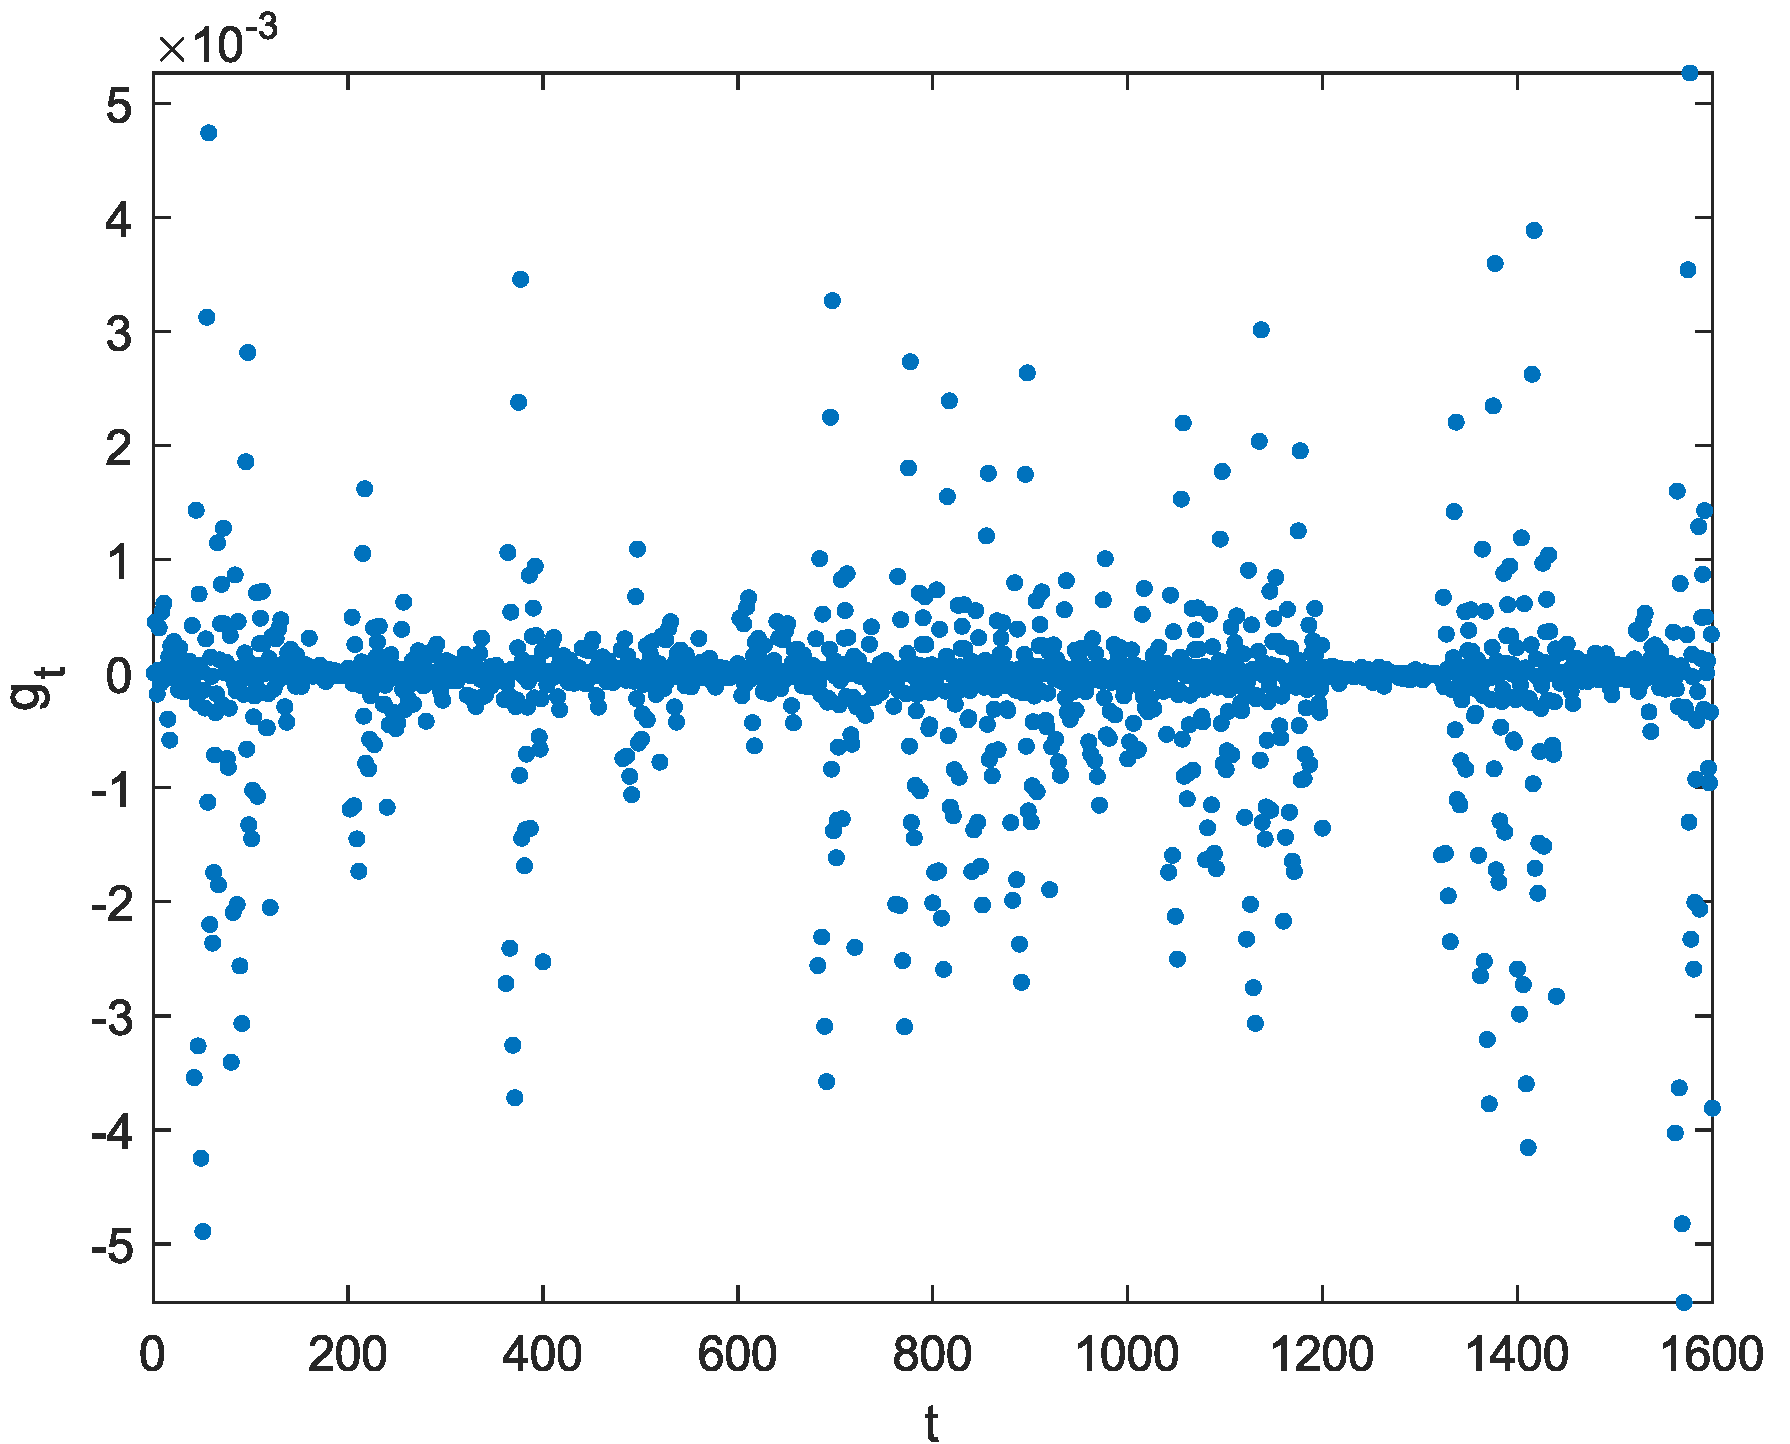
\includegraphics[width=0.47\linewidth]{gradient-gcac-a.pdf}
        \label{fig_Gradient-Distribution-Before-Compression-1}
    }
    \subfloat[压缩后梯度分布]{
        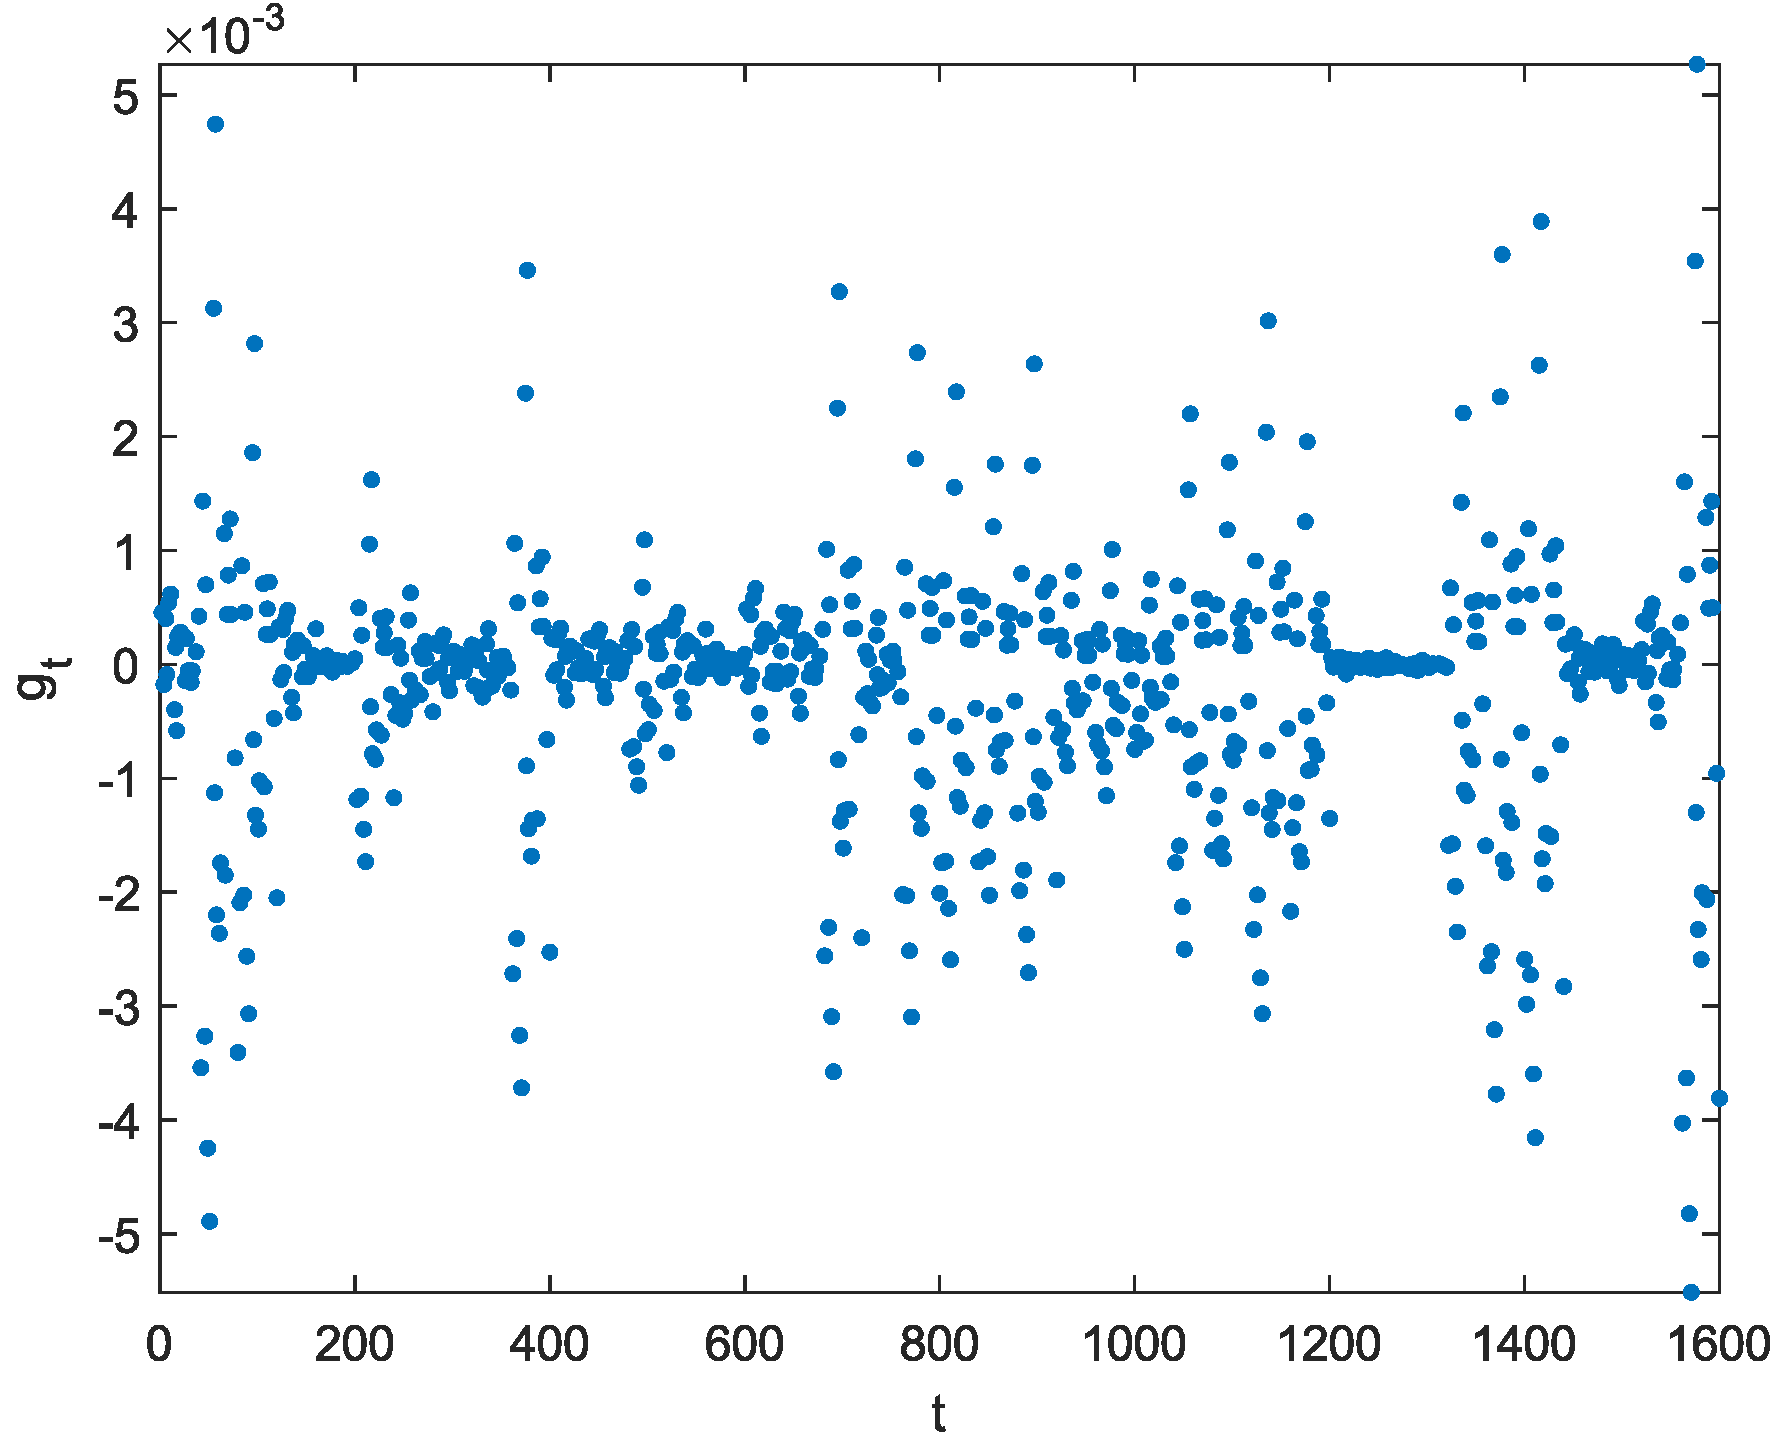
\includegraphics[width=0.47\linewidth]{gradient-gcac-b.pdf}
        \label{fig_Gradient-Distribution-After-Compression-1}
    } \\
    \subfloat[对应(a)图,压缩前梯度极坐标分布]{
        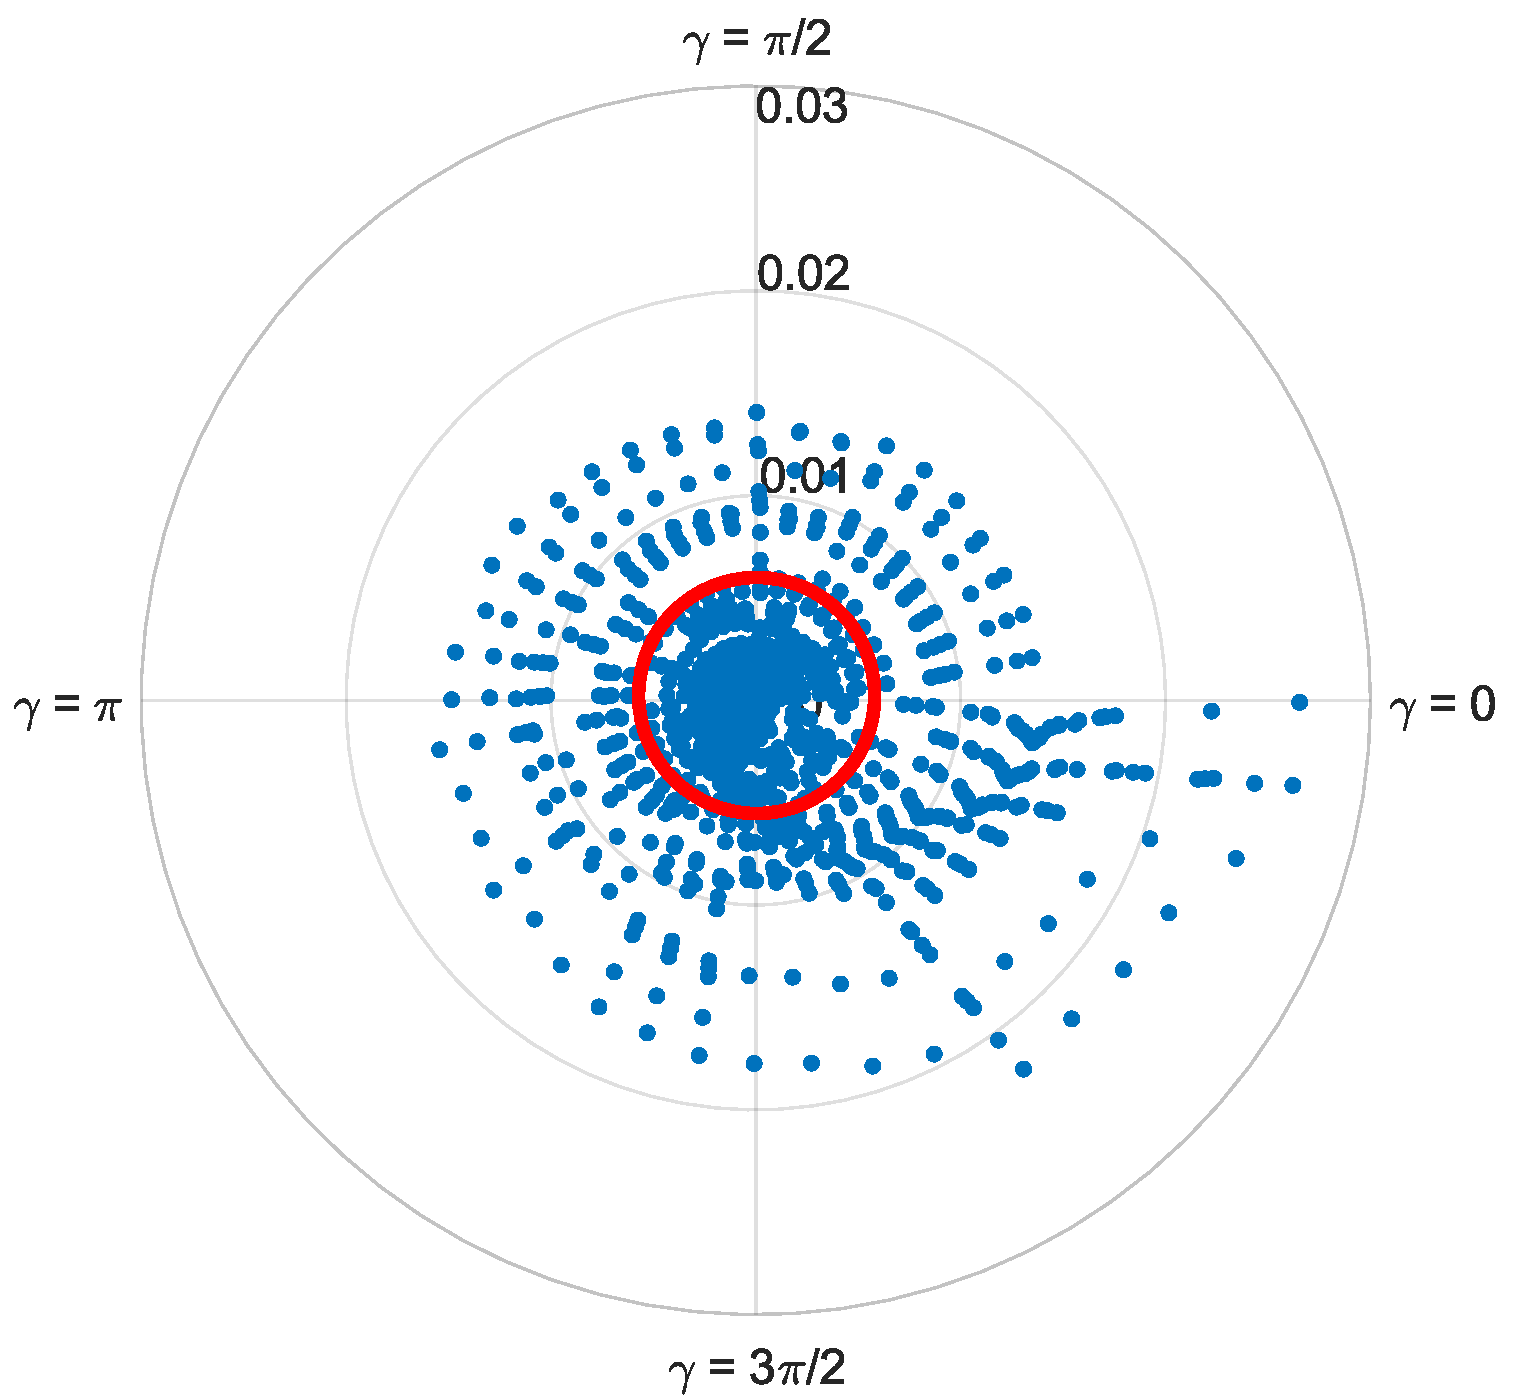
\includegraphics[width=0.47\linewidth]{gradient-gcac-c.pdf}
        \label{fig_Gradient-Distribution-Before-Compression-2}
    }
    \subfloat[对应(b)图,压缩后梯度极坐标分布]{
        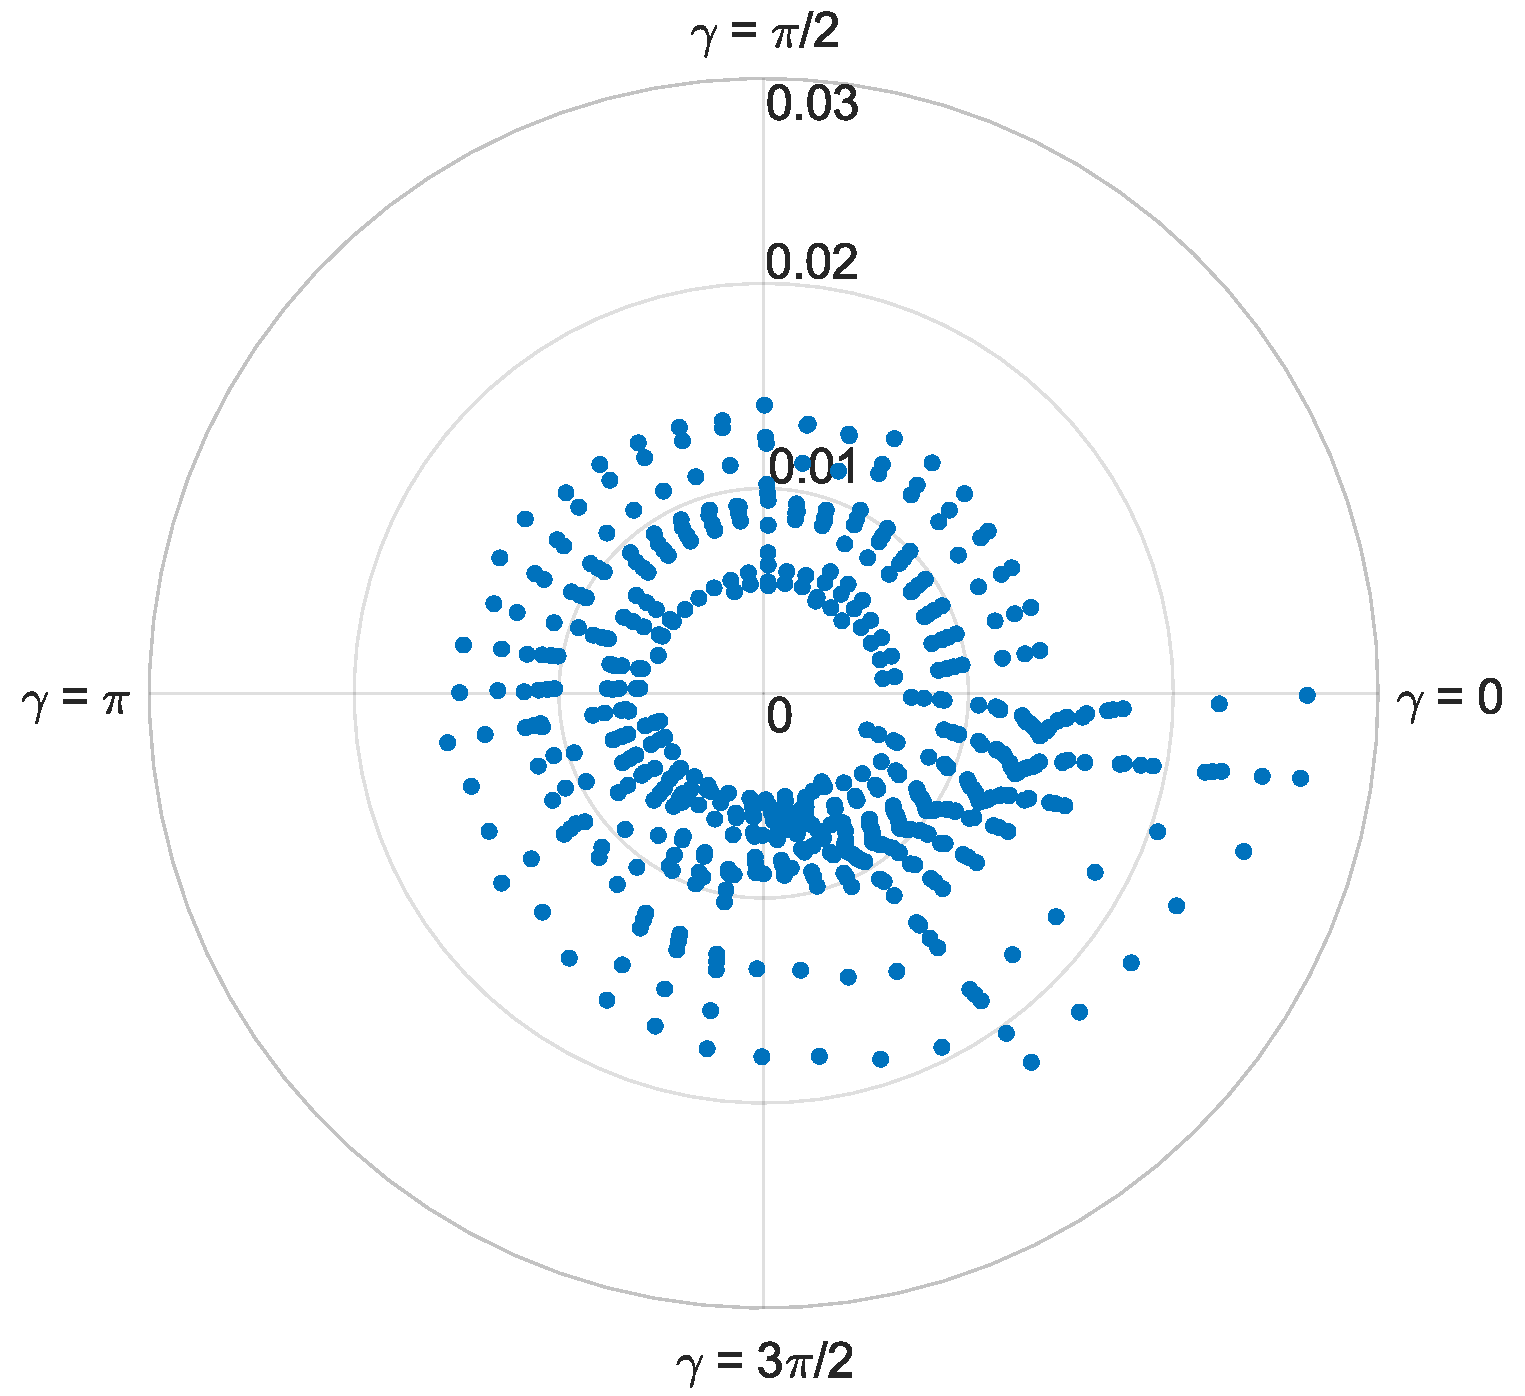
\includegraphics[width=0.47\linewidth]{gradient-gcac-d.pdf}
        \label{fig_Gradient-Distribution-After-Compression-2}
    } \\
    \caption{基于GCAC算法压缩前后梯度分布}
    \label{fig_Gradient-Compression-Distribution-2}
\end{figure}
%%%%%%%%%%%%%%%%%%%%%%%%%%%%%%%%%%%%%%%
我们针对获取到的的梯度进行了简单变换操作,即将笛卡尔坐标系中的梯度分布情况同步到极坐标中。
极角通过公式 \eqref{eq_Gradient-transform} 转换得到,极径为当前梯度$g$与近似质心$\hat{\mathcal{C}}^{m[k]}$之间的欧式距离$s_t^{m[k]}$:
%%%%%%%%%%%%%%%%%%%%%%%%%%%%%%%%%%%%%%%
\begin{equation}
    \begin{aligned}
        \gamma &= \frac{2\pi}{t}, \\
        s_t^{m[k]} &= \phi \left(\hat{\mathcal{C}}^{m[k]}, g_{t}^{m[k]} \right)
    \end{aligned}
    \label{eq_Gradient-transform}
\end{equation}
%%%%%%%%%%%%%%%%%%%%%%%%%%%%%%%%%%%%%%%

在图 \ref{fig_Gradient-Compression-Distribution-2} 的 (a) 和 (c) 子图中,不难发现,
绝大多数的梯度都分布在较小的范围内,并且十分接近该局部梯度矩阵质心,
所以这些梯度可以被那些远离质心的梯度进行表示,也就是说,当梯度压缩比较大时,仍然不会对神经网络模型性能优化产生较大影响。
图 \ref{fig_Gradient-Compression-Distribution-2} (c) 中红色圆圈对应于图 \ref{fig_Gradient-Distribution-1} (a) 中红色点状线,它们梯度压缩比都是2。
显然,圈内的梯度更加接近局部梯度矩阵的质心,它们包含高度相似的信息,并且可以通过圆外的梯度(即远离质心的梯度)进行线性组合获得,因此,他们对模型参数更新的贡献可被替代,对它们实施裁剪操作并不会对网络模型性能产生实质性的影响。

如图 \ref{fig_Gradient-Compression-Distribution-2} (b) 和 图\ref{fig_Gradient-Compression-Distribution-2} (d) 所示,
与基于梯度值或范数的梯度压缩方法(见图 \ref{fig_Gradient-Distribution-1} (b))相比,
当采用GCAC算法时,其结果保留了相对相对较大和相对较小的梯度,
因此即使不满足上述两个隐含条件,也保留了大部分重要的梯度信息。

\section{实验与结果分析}
\label{sec_ResultAndAnalisy}
\subsection{实验环境以及相关参数配置}
\label{sec_EnvironmentAndHyperParameterSet}
本章所有的验证实验都将部署在由4个Worker节点构成的Linux集群环境下。具体来说,单个Worker节点的主要硬件环境包括:
CPU处理器为主频4.50 GHz的Intel® Core™ i9-10900X、内存大小为64 GB、GPU采用的是显存大小为11 GB的GeForce GTX 2080Ti,网络接口设备带宽为1000 Mb/s。
另外,为了便于部署与管理分布式集群中各个节点实验环境,采用Docker 20.10进行镜像封装,且镜像内部主要装有OpenMPI 4.0、CUDA 11.7、Python 3.8、PyTorch 1.7以及Horovod 0.21等软件。
另外,针对高光谱目标检测任务,运行在Linux操作系统上的MATLAB 2021b被用来进行输入数据的预处理以及输出结果的后处理操作。

当处理不同的下游任务时,我们采取了不同的神经网络模型和数据集,关于下游任务、网络模型以及相关数据集具体设置如表 \ref{tab_Network4task} 所示。
另外,分布式训练部署过程涉及众多超参数设置,主要包括Batch 大小$\varphi$、
最大迭代轮数$Epochs$、学习率$\eta$、动量Momentum、权重衰减因子、优化器等,实验实施过程中需要针对不同数据集进行不同超参数设置,具体设置如表 \ref{tab_Network-Parameter} 所示。
另外,需要注意的是,当采用AAE网络模型时,其中AE子网络结构采用对称结构,编码器中隐藏层数量设置为2,每一个隐藏层神经元数量设置为1000。

%%%%%%%%%%%%%%%%%%%%%%%%%%%%%%%%%%%%%%%
\renewcommand{\arraystretch}{1.3}
\begin{table*}[ht]
    \centering
    \begin{threeparttable}
        \caption{下游任务、网络模型以及训练数据集相关设置}
        \label{tab_Network4task}
        \begin{tabular}{c|c|c}
            \toprule
            \toprule
            下游任务 & 网络模型 & 数据集 \\
            \midrule
            \multirow{2}{*}{高光谱目标检测} & \multirow{2}{*}{AAE} & AeroRIT \\
                    &         & Xiongan New Area(Matiwan Village) \\
            \midrule
            \multirow{3}{*}{图像分类} & VGGNet-16 & \multirow{3}{*}{CIFAR10} \\
                                    & ResNet-56 & \\
                                    & ResNet-110 & \\
            \bottomrule
            \bottomrule
        \end{tabular}
    \end{threeparttable}
\end{table*}
%%%%%%%%%%%%%%%%%%%%%%%%%%%%%%%%%%%%%%%

%%%%%%%%%%%%%%%%%%%%%%%%%%%%%%%%%%%%%%%
\renewcommand{\arraystretch}{1.3}
\begin{table*}[ht]
    \centering
    \begin{threeparttable}
        \caption{GCAC梯度压缩算法超参数设置}
        \label{tab_Network-Parameter}
        \begin{tabular}{c|c|c|c|c|c|c}
            \toprule
            \toprule
            数据集 & $Bs$& $Epochs$ & 学习率$\eta$ & 动量 & 权重衰减因子 & 优化器 \\
            \midrule
            AeroRIT & 310000 & 100 & \multirow{3}{*}{0.0001} & \multirow{3}{*}{-} & \multirow{3}{*}{-} & \multirow{3}{*}{Adam} \\
            Xiongan New Aera & \multirow{2}{*}{200000} &  \multirow{2}{*}{200} & & &  & \\
            (Matiwan Village) &  & & & & & \\
            \midrule
            CIFAR10 & 128 & 200 & 0.01 & 0.9 & 0.0005 & SGD \\
            \bottomrule
            \bottomrule
        \end{tabular}
    \end{threeparttable}
\end{table*}
%%%%%%%%%%%%%%%%%%%%%%%%%%%%%%%%%%%%%%%

\subsection{高光谱目标检测实验结果分析}
为了验证本章提出的梯度压缩算法的可行性,首先选择高光谱目标检测作为下游任务进行验证。
如图 \ref{fig_Result-AeroRIT} 所示,针对AeroRIT高光谱数据集,我们分别考察了不同压缩比和梯度压缩算法对高光谱目标检测结果的影响。
其中,图 \ref{fig_Result-AeroRIT} \subref{fig_Result-AeroRIT-pseudo-color} 展示了该场景的伪彩图,
而图 \ref{fig_Result-AeroRIT} \subref{fig_Result-AeroRIT-ground-truth} 则描述了该场景中感兴趣目标的分布情况,
图 \ref{fig_Result-AeroRIT} \subref{fig_Result-AeroRIT-baseline} 给出了不进行梯度压缩的情况下,对AeroRIT数据集进行分布式训练的效果图,
图 \ref{fig_Result-AeroRIT} \subref{fig_Result-AeroRIT-gcc-cr0.1}、\subref{fig_Result-AeroRIT-gcc-cr0.01}
分别展示了在压缩比$cr$分别设置为10、100的情况下,采用本章提出的梯度压缩算法(GCAC)时的检测效果图,
图 \ref{fig_Result-AeroRIT} \subref{fig_Result-AeroRIT-l1-cr0.1} 展示了在压缩比$cr$设置为10,且以L1-范数作为梯度重要性度量的情况下,进行目标检测的效果图,
图 \ref{fig_Result-AeroRIT} \subref{fig_Result-AeroRIT-dgc-cr0.1} 、图 \ref{fig_Result-AeroRIT} \subref{fig_Result-AeroRIT-Topk-cr0.1} 分别展示了在压缩比$cr$设置为10的情况下,采用DGC、Top-K算法进行分布式训练的检测效果图。

%%%%%%%%%%%%%%%%%%%%%%%%%%%%%%%%%%%%%%%
\begin{figure}[H]
    \centering
    \subfloat[伪彩图]{
        \includegraphics[width=0.473\linewidth]{aerorit-pseudo-color.pdf}
        \label{fig_Result-AeroRIT-pseudo-color}
    }
    \subfloat[Ground truth]{
        
\includegraphics[width=0.473\linewidth]{aerorit-ground-truth.pdf}
        \label{fig_Result-AeroRIT-ground-truth}
    } \\
    \subfloat[Baseline]{
        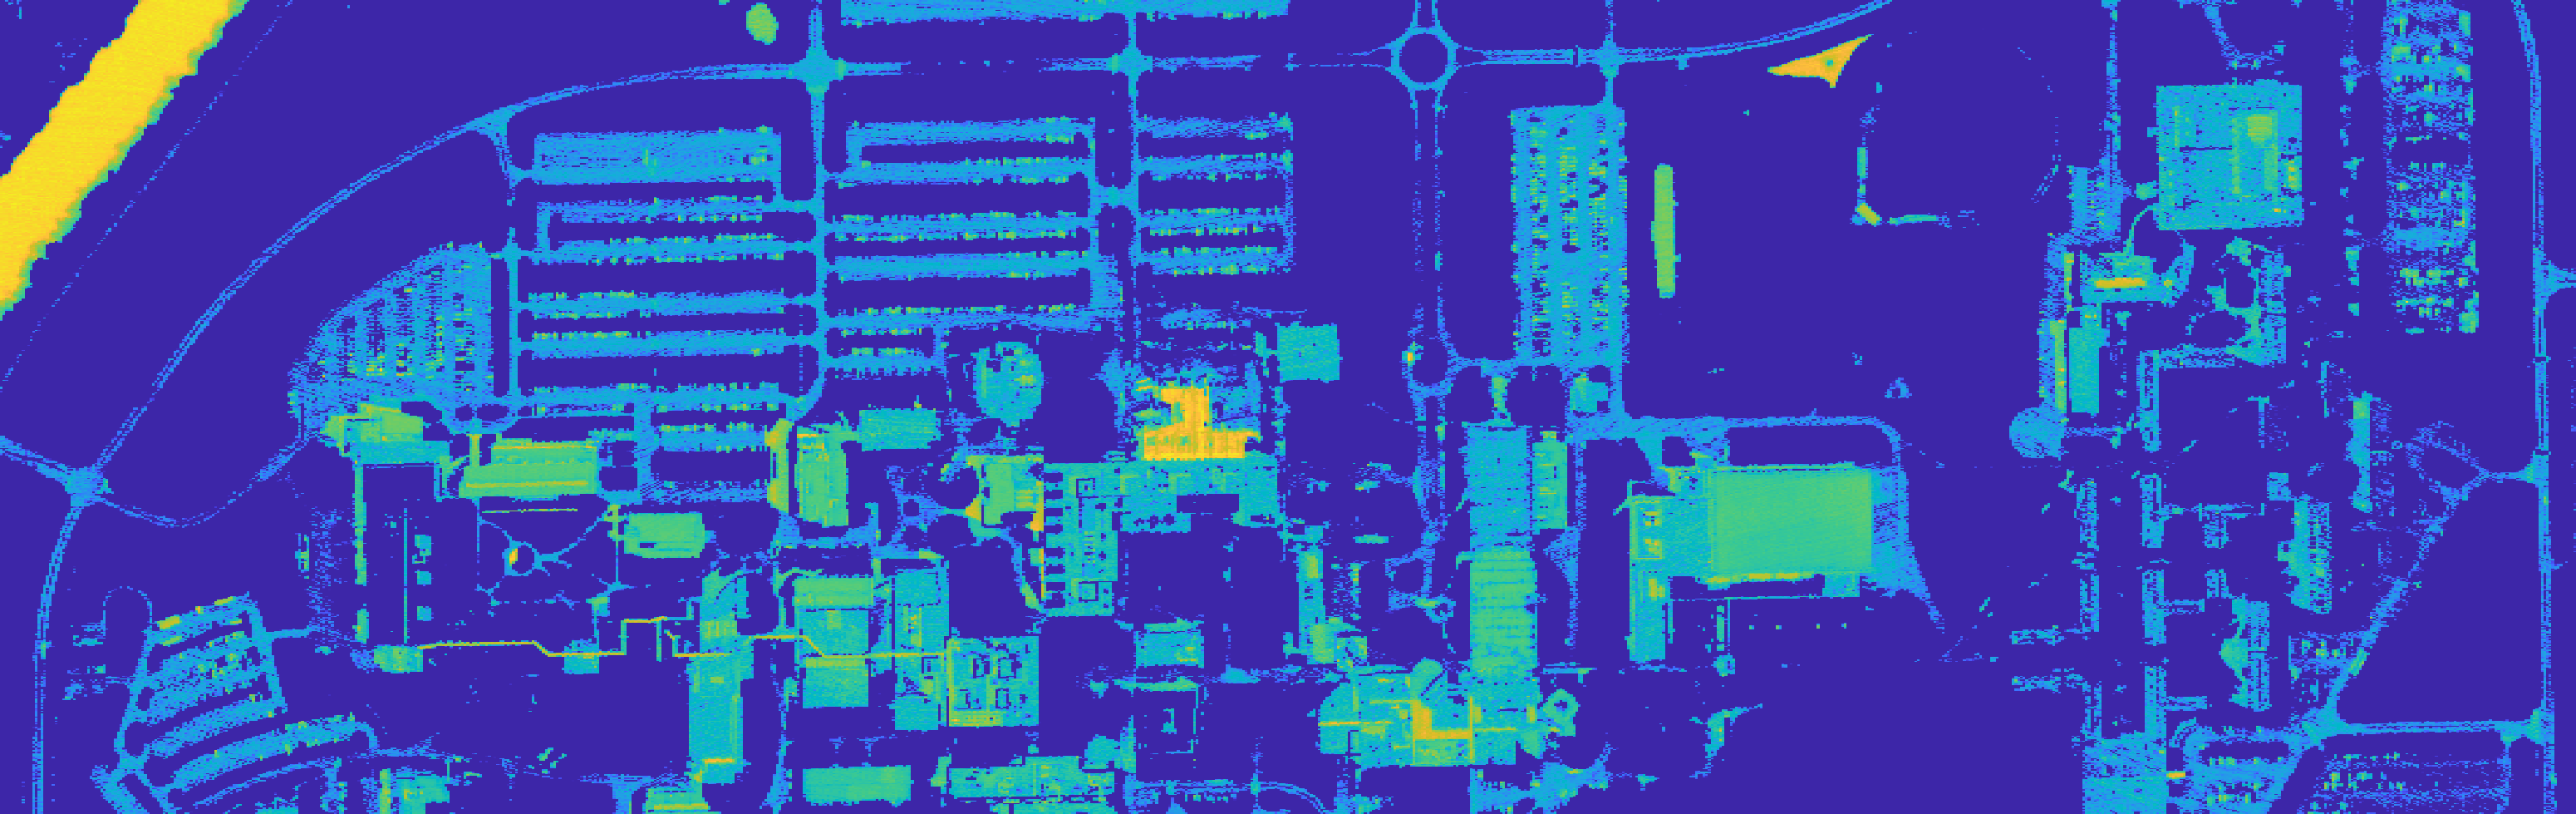
\includegraphics[width=0.473\linewidth]{aerorit-base-line.pdf}
        \label{fig_Result-AeroRIT-baseline}
    }
    \subfloat[GCAC: $cr=10$]{
        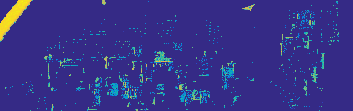
\includegraphics[width=0.473\linewidth]{aerorit-gcc-cr0.1.pdf}
        \label{fig_Result-AeroRIT-gcc-cr0.1}
    } \\
    \subfloat[GCAC: $cr=100$]{
        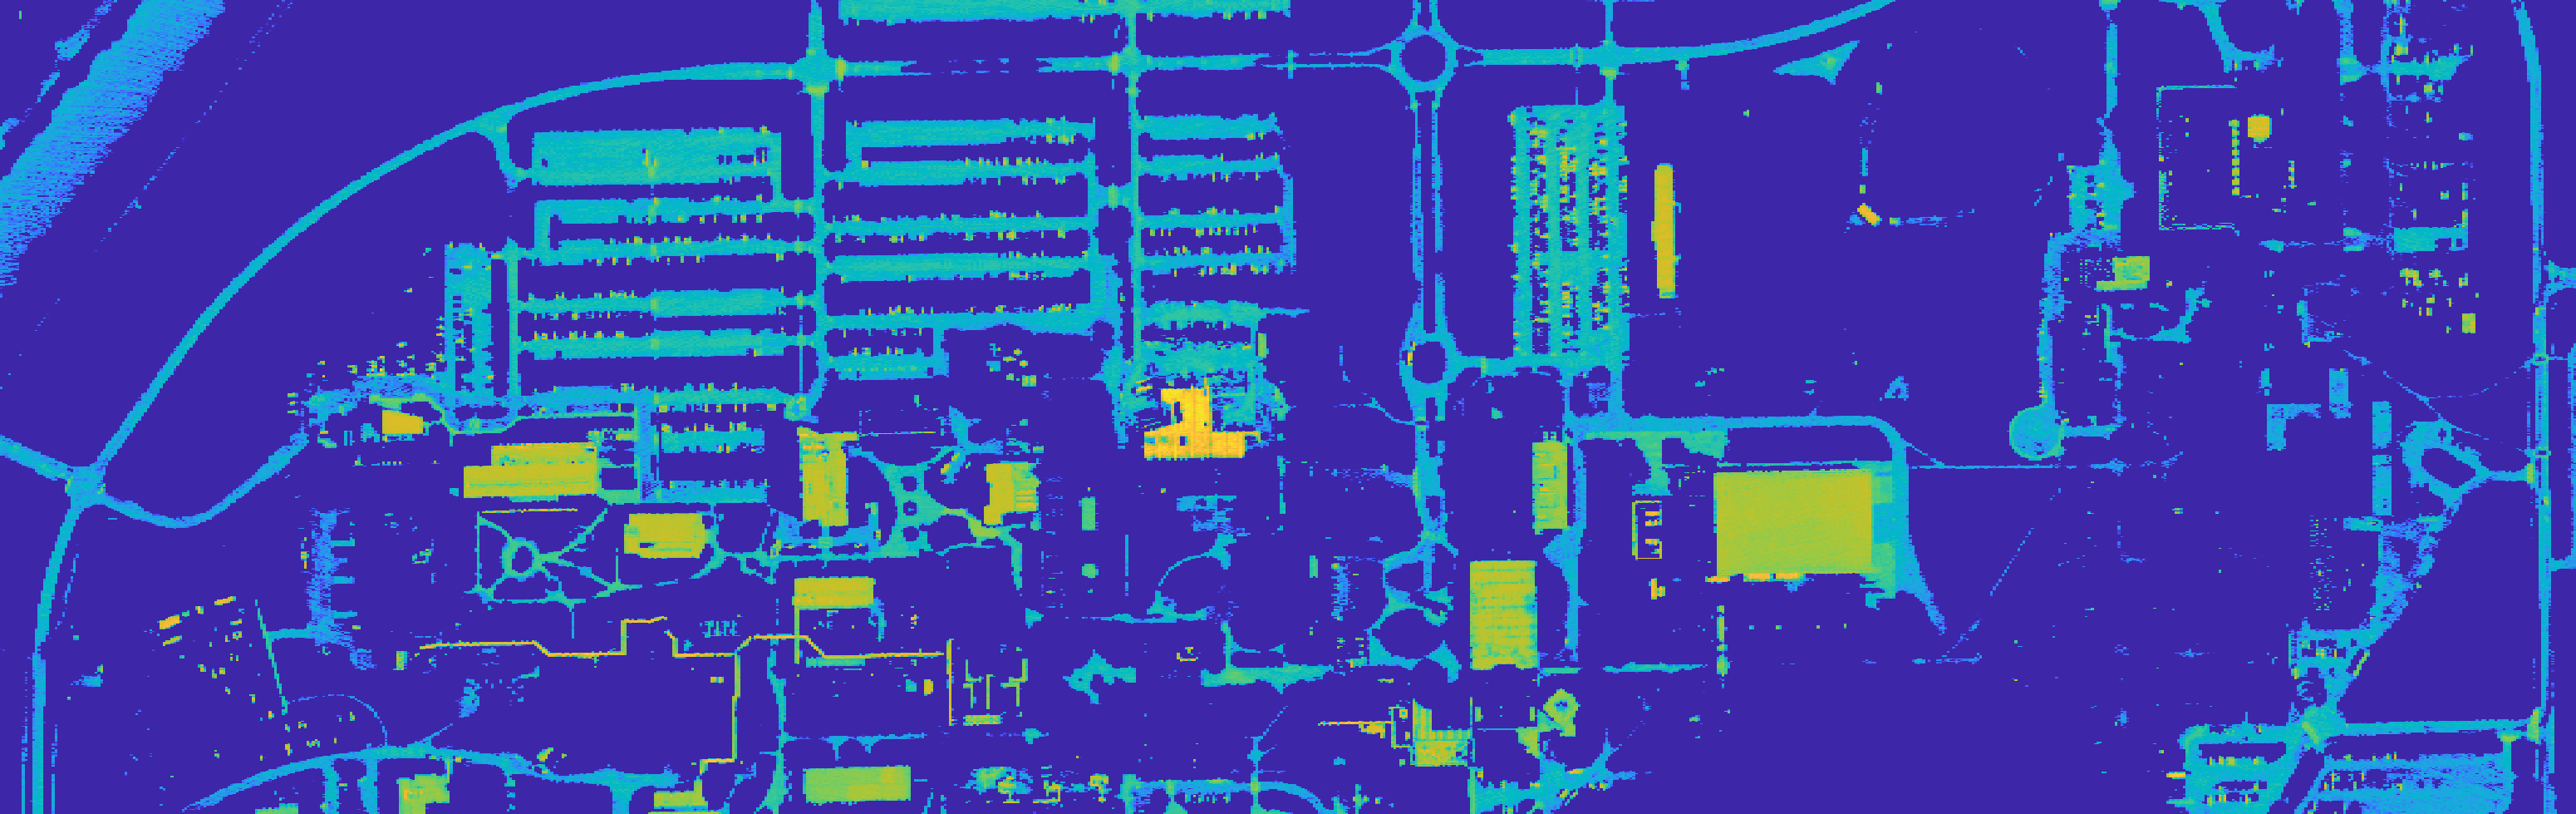
\includegraphics[width=0.473\linewidth]{aerorit-gcc-cr0.01.pdf}
        \label{fig_Result-AeroRIT-gcc-cr0.01}
    }
    \subfloat[L1: $cr=10$]{
        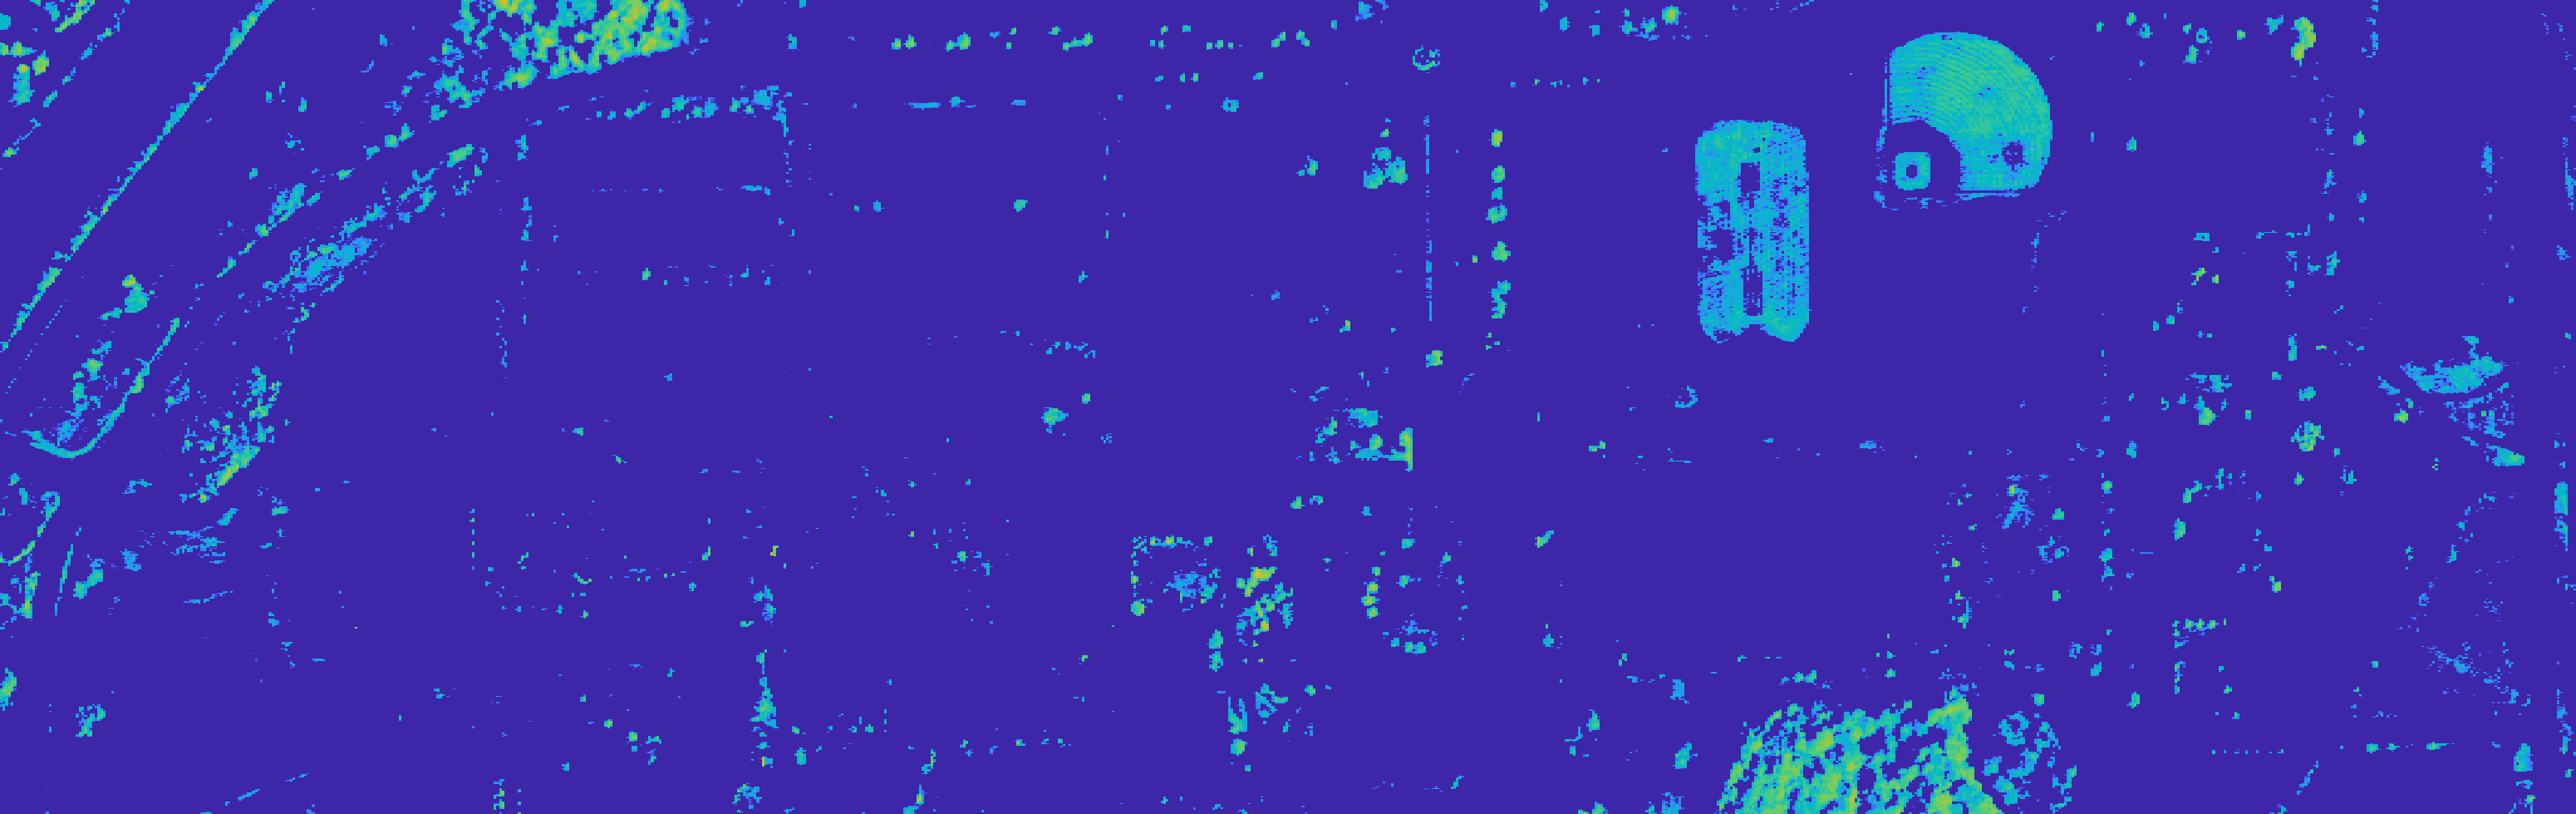
\includegraphics[width=0.473\linewidth]{aerorit-l1-cr0.1.pdf}
        \label{fig_Result-AeroRIT-l1-cr0.1}
    } \\
    \subfloat[DGC: $cr=10$]{
        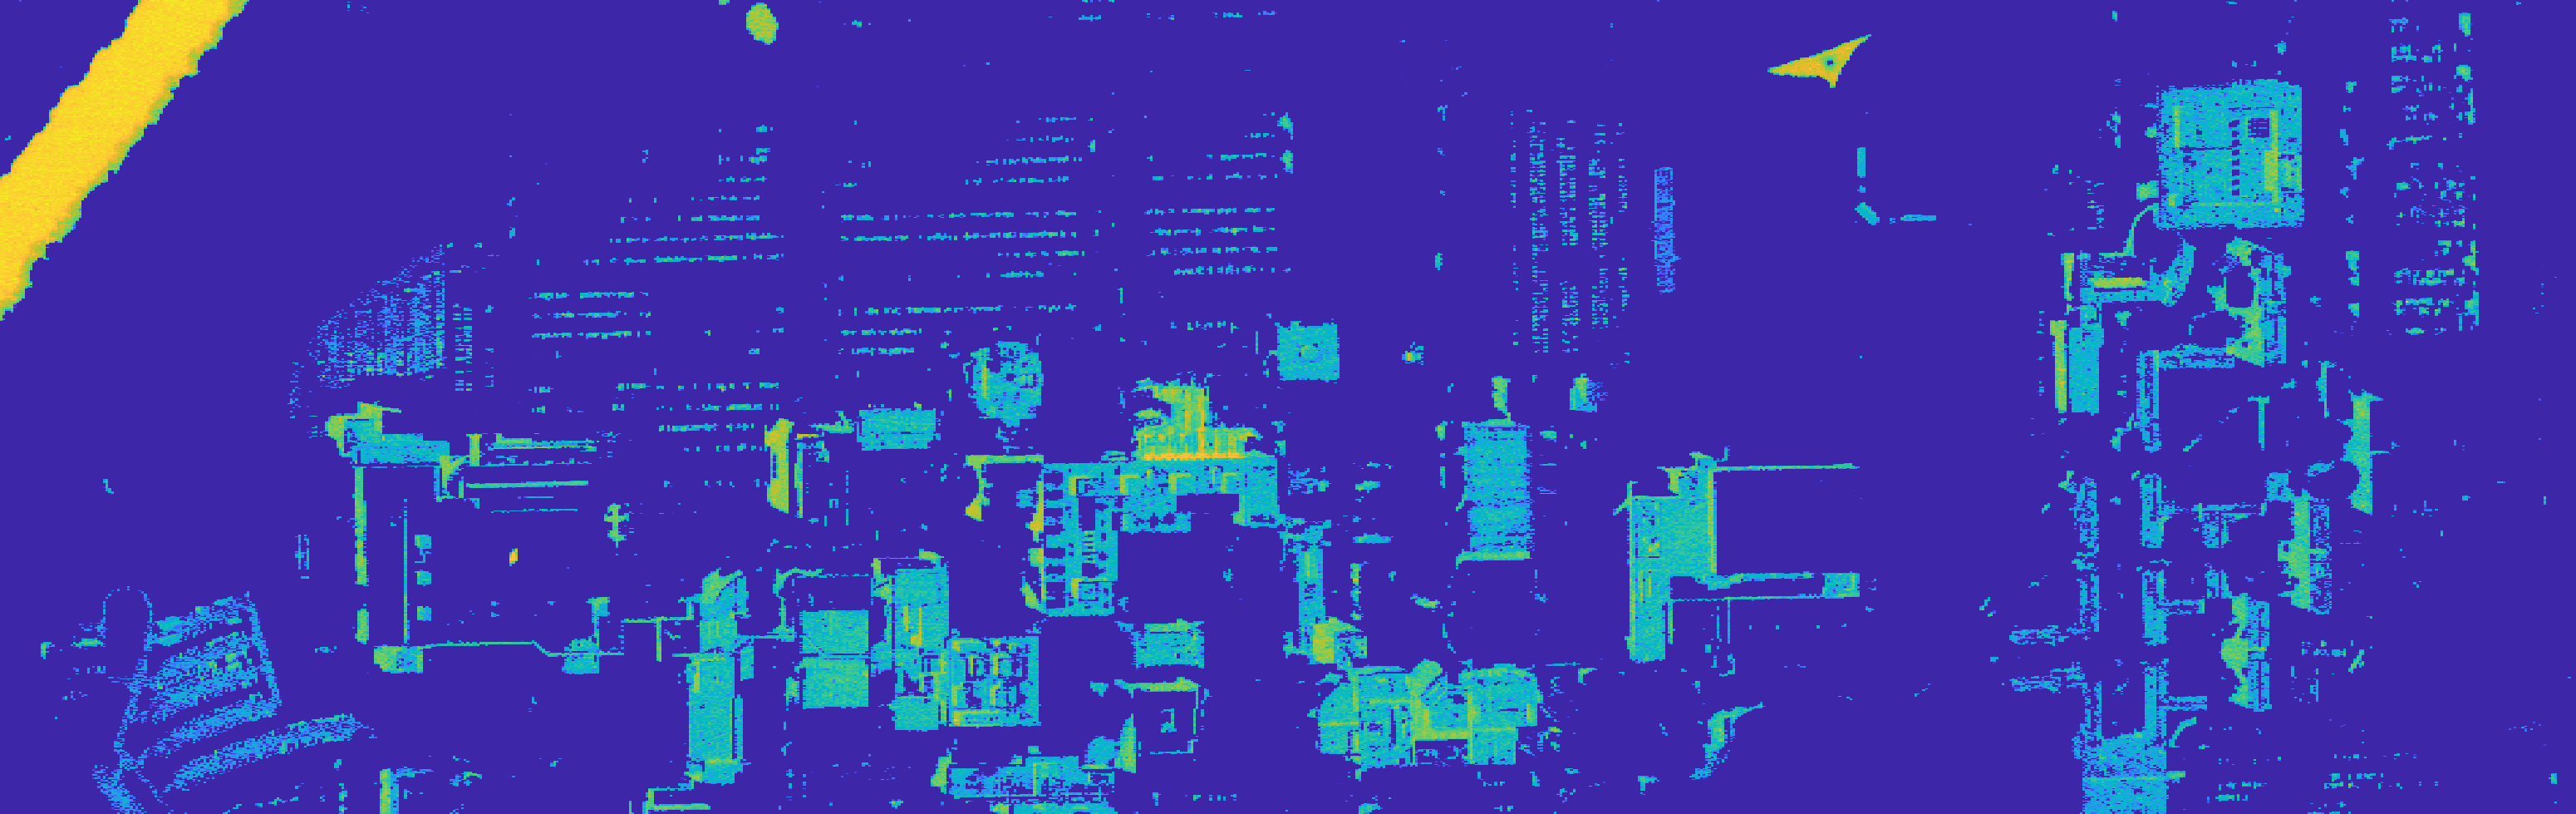
\includegraphics[width=0.473\linewidth]{aerorit-dgc-cr0.1.pdf}
        \label{fig_Result-AeroRIT-dgc-cr0.1}
    }
    \subfloat[Top-K: $cr=10$]{
        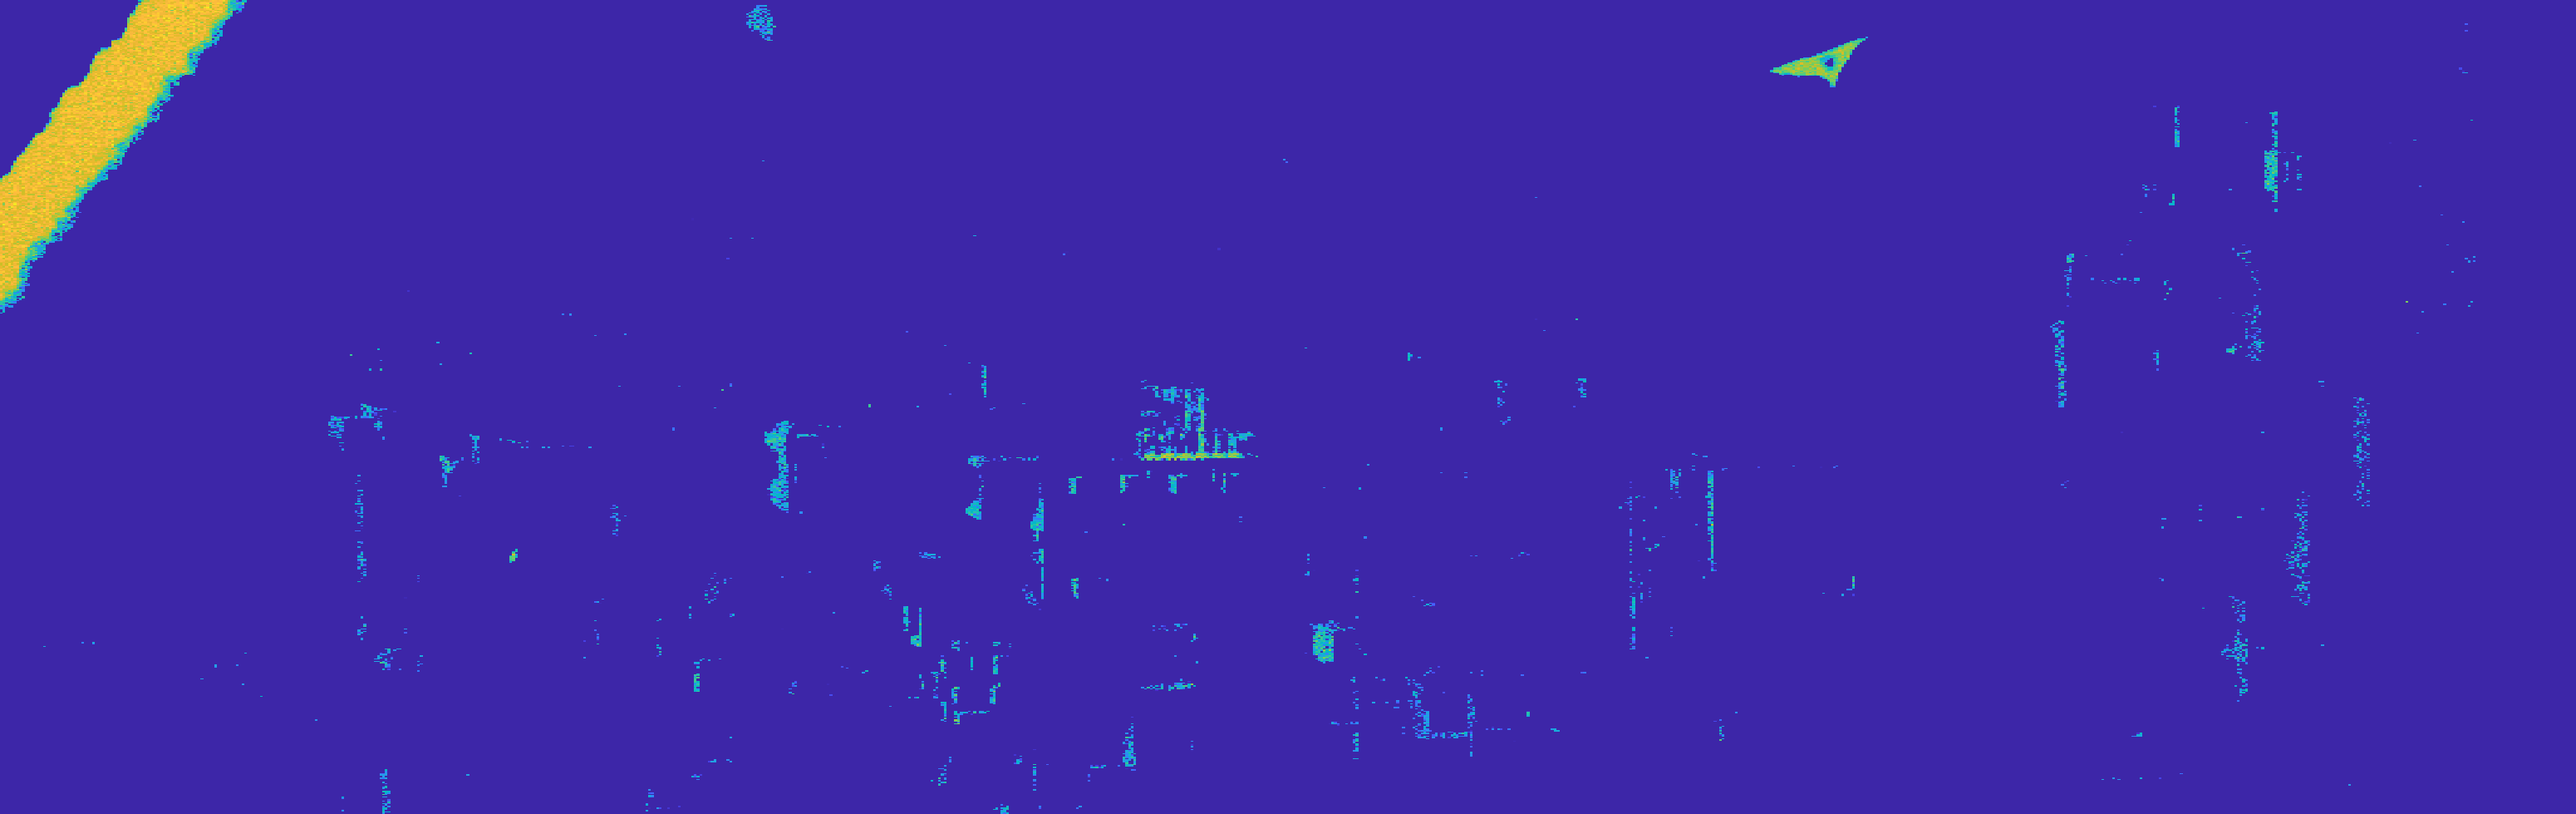
\includegraphics[width=0.473\linewidth]{aerorit-topk-cr0.1.pdf}
        \label{fig_Result-AeroRIT-Topk-cr0.1}
    }
    \caption{AeroRIT数据集上,使用不同梯度压缩算法进行分布式训练的高光谱目标检测可视化结果}
    \label{fig_Result-AeroRIT}
\end{figure}
%%%%%%%%%%%%%%%%%%%%%%%%%%%%%%%%%%%%%%%

在高光谱目标检测任务中,我们不仅仅在AeroRIT数据集上进行实验,
同时也在规模更大的遥感数据集Xiongan New Area(Matiwan Village)上进行了验证。
图 \ref{fig_Result-Xiongan} 展示了分布式训练的高光谱目标检测效果对比。
其中,
\subref{fig_Result-Xiongan-pseudo-color} $\thicksim$ \subref{fig_Result-Xiongan-top-k-cr0.1}
子图分别展示了高光谱数据集Xiongan New Area(Matiwan Village)的伪彩图、感兴趣目标的真实标签分区情况(Ground truth)、不进行梯度压缩的高光谱目标检测效果图(Baseline)、
采用GCAC算法并设置压缩比$cr$为10和100的情况下,进行高光谱目标检测效果图,以及压缩比$cr$为10的情况下,采用L1-范数作为梯度重要性度量、DGC、Top-K等梯度压缩算法的高光谱目标检测效果图。

%%%%%%%%%%%%%%%%%%%%%%%%%%%%%%%%%%%%%%%
\begin{figure}[ht]
    \centering
    \subfloat[伪彩图]{
        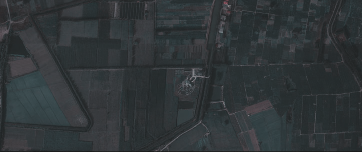
\includegraphics[width=0.485\linewidth]{xiongan-pseudo-color.pdf}
        \label{fig_Result-Xiongan-pseudo-color}
    }
    \subfloat[Ground truth]{
        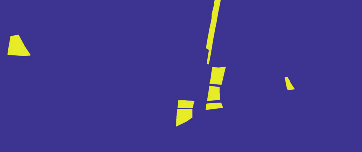
\includegraphics[width=0.485\linewidth]{xiongan-ground-truth.pdf}
        \label{fig_Result-Xiongan-ground-truth}
    } \\
    \subfloat[Baseline]{
        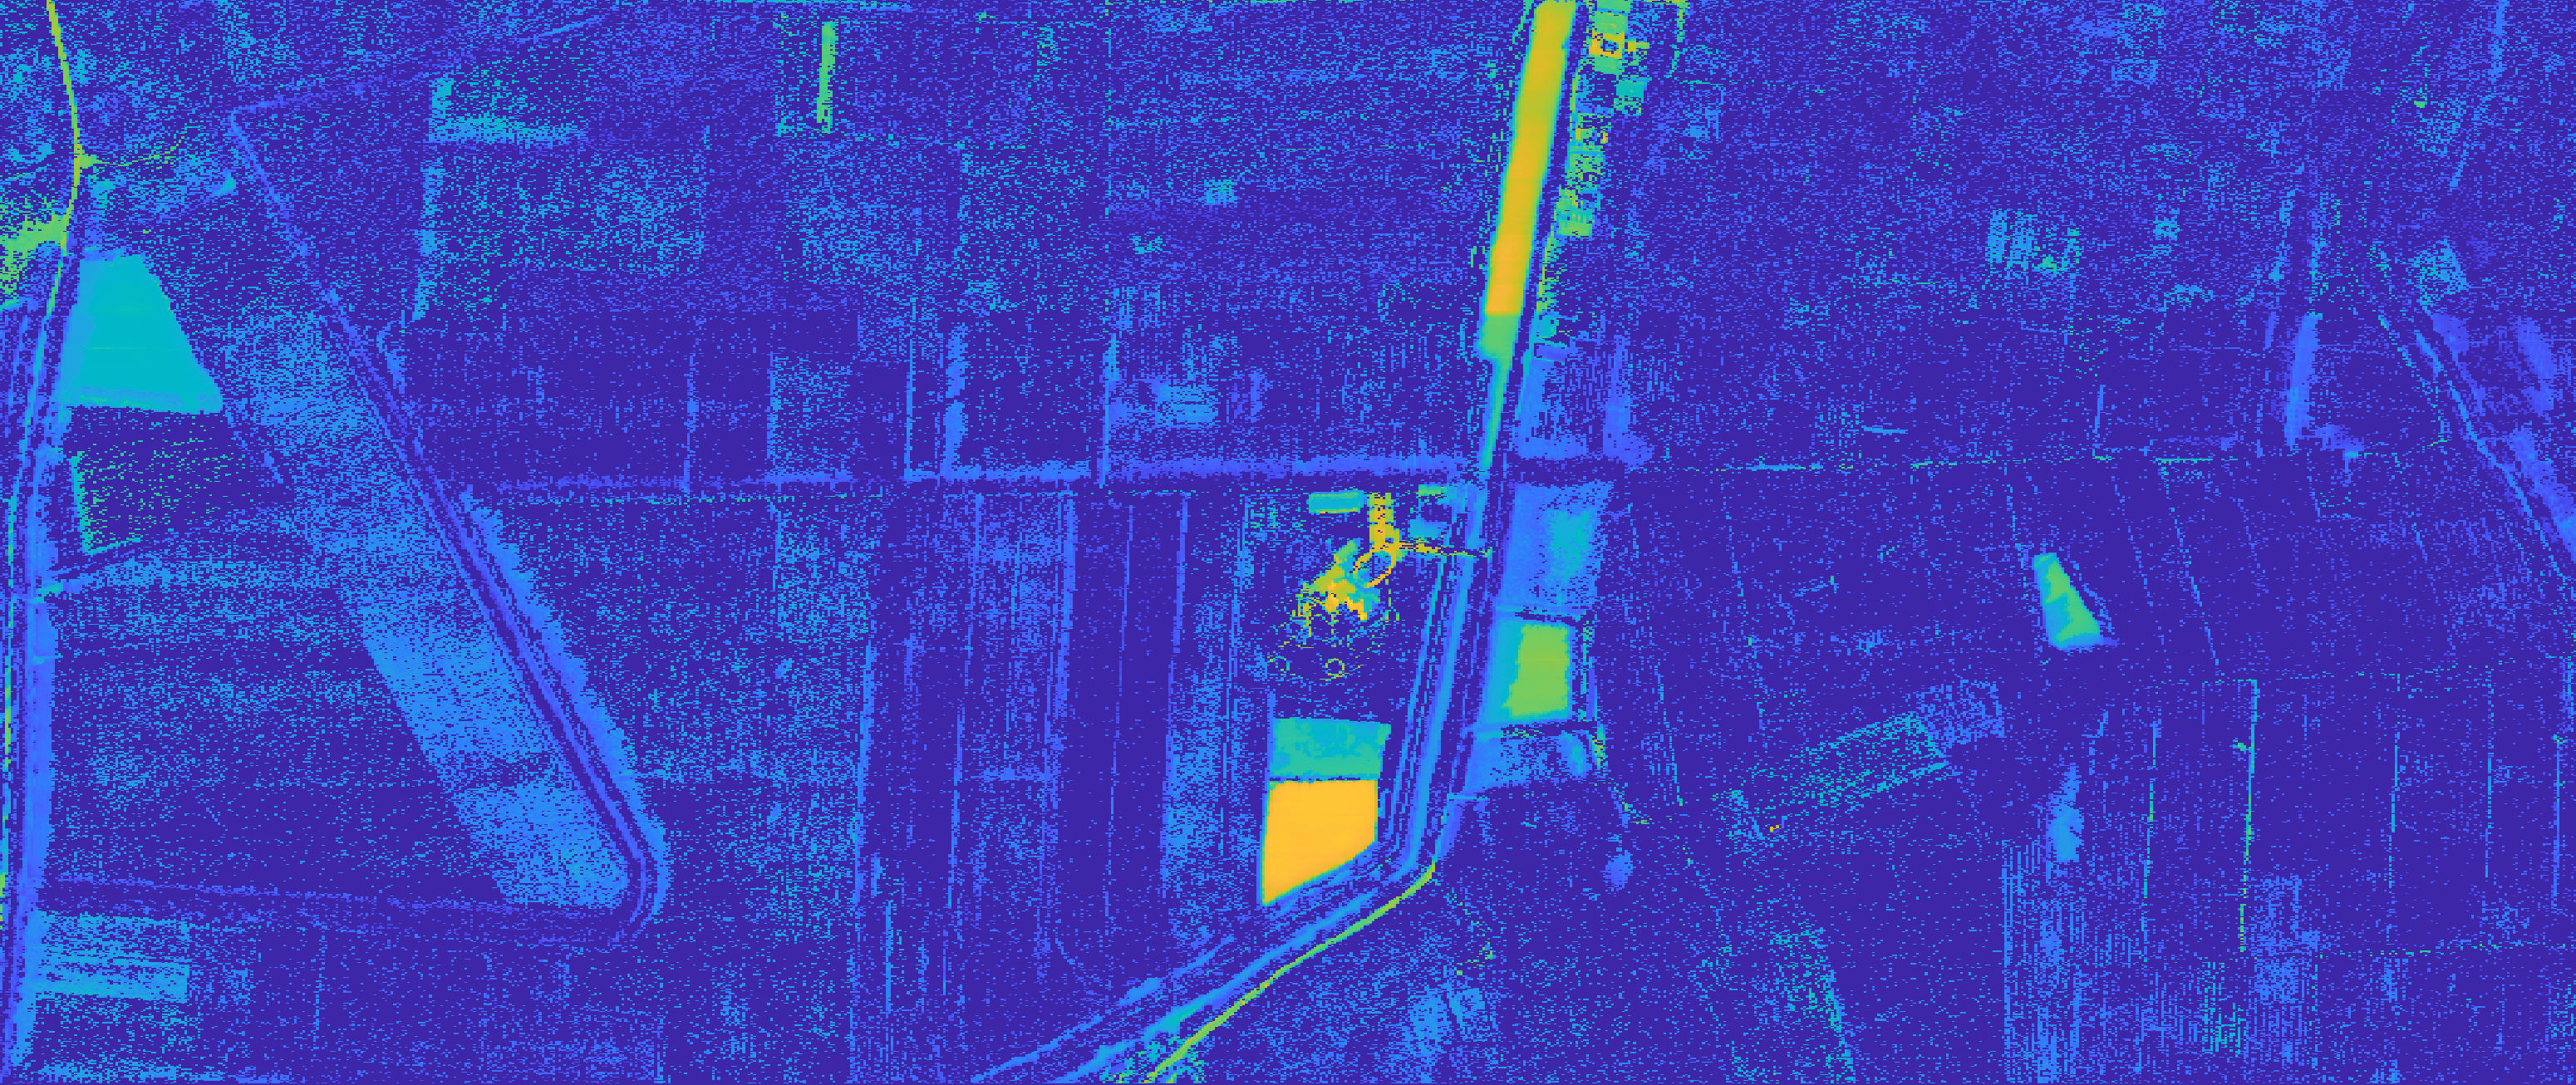
\includegraphics[width=0.485\linewidth]{xiongan-base_line.pdf}
        \label{fig_Result-Xiongan-baseline}
    }
    \subfloat[GCAC: $cr=10$]{
        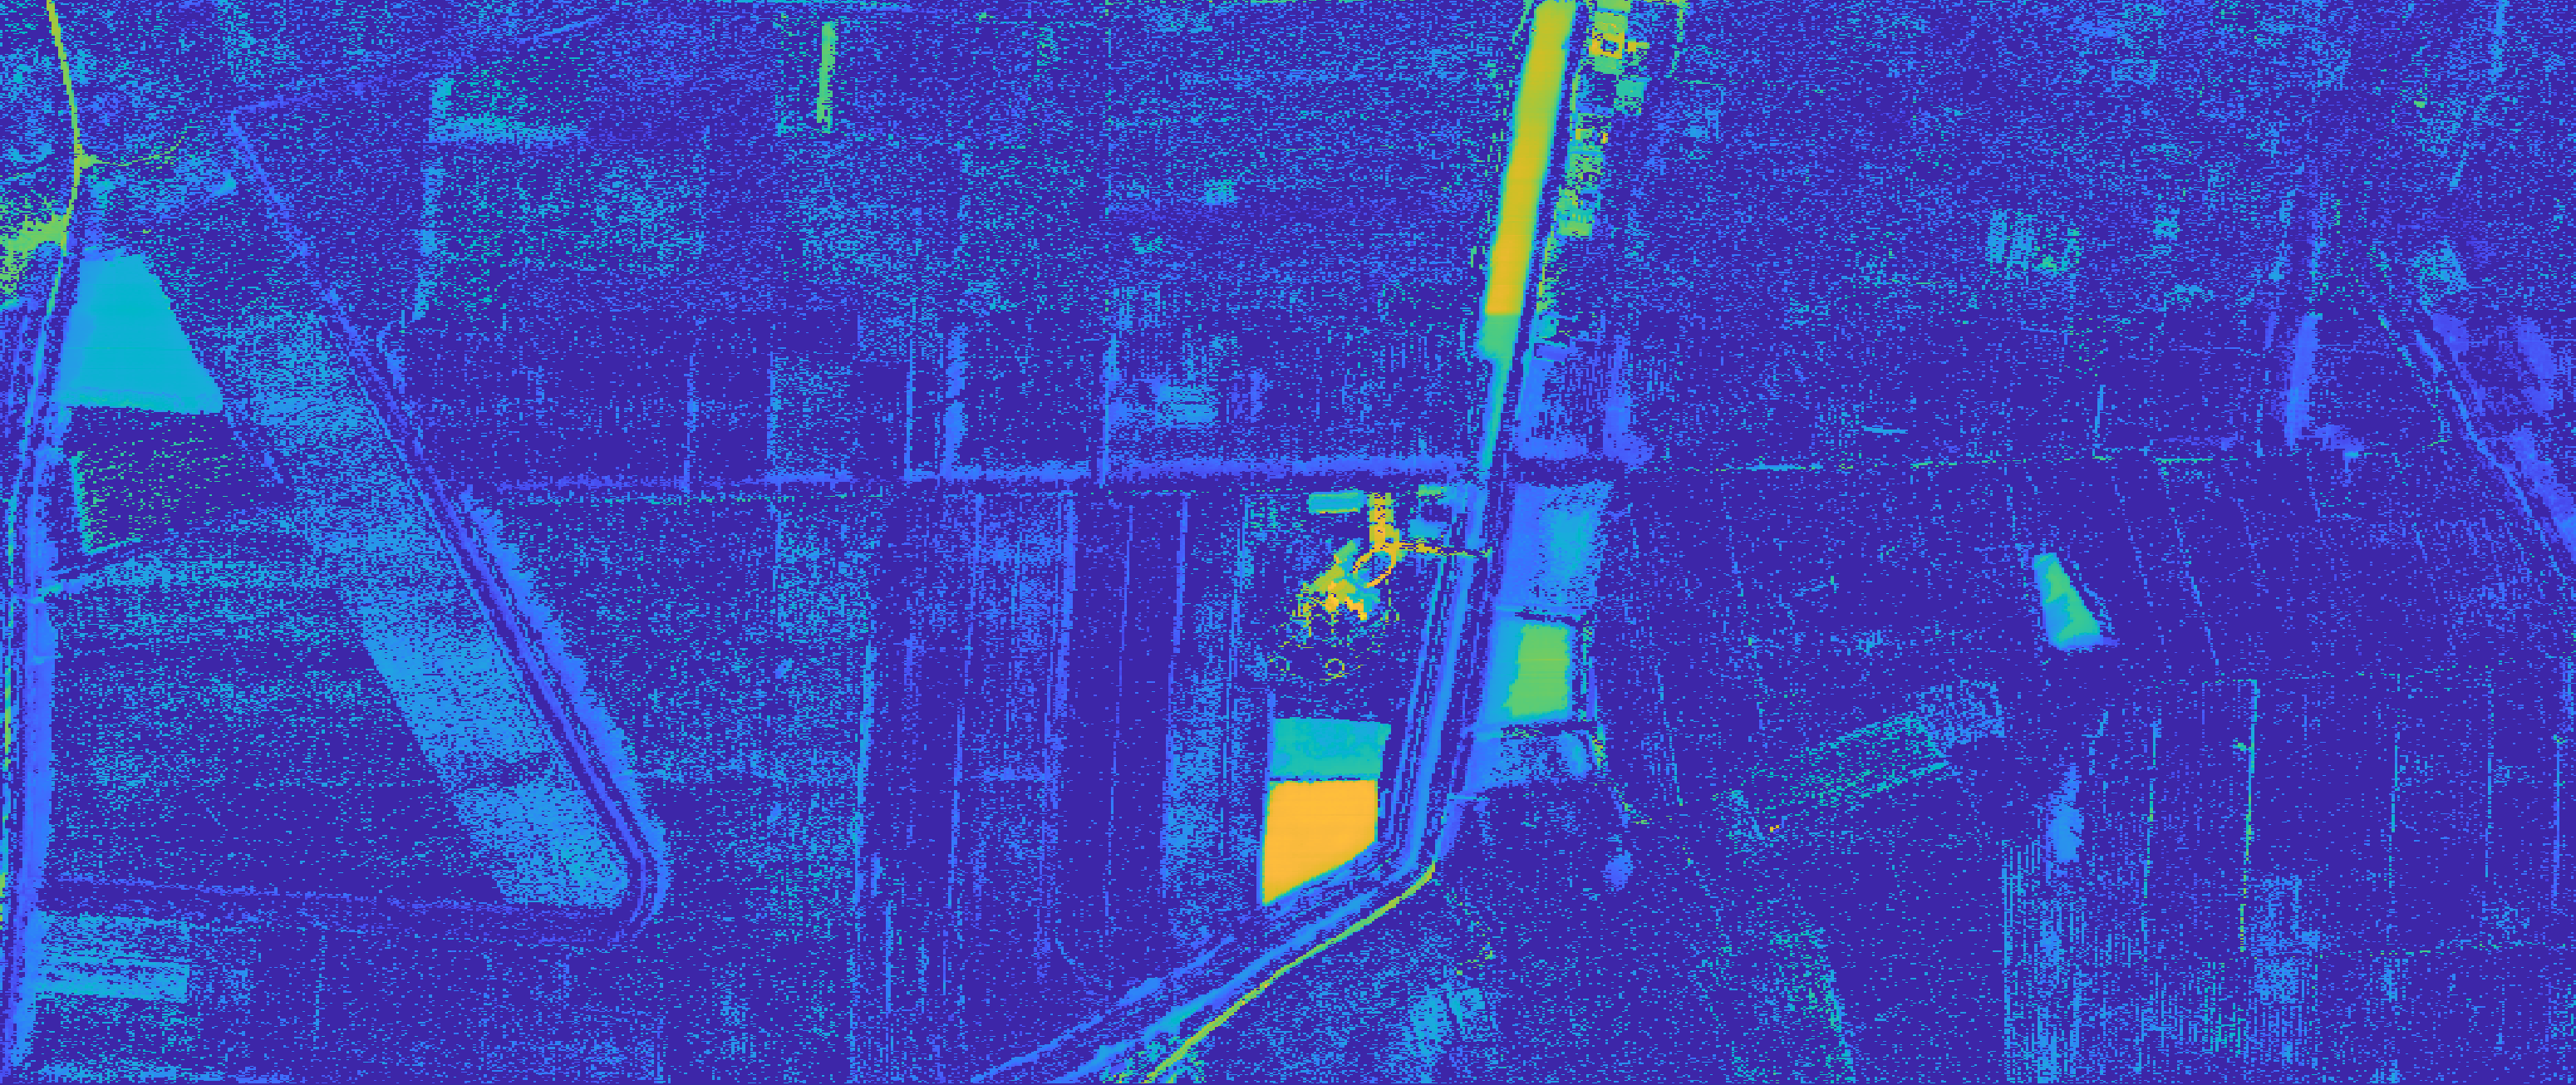
\includegraphics[width=0.485\linewidth]{xiongan-gcac_cr10.pdf}
        \label{fig_Result-Xiongan-gcc-cr0.1}
    } \\
    \subfloat[GCAC: $cr=100$]{
        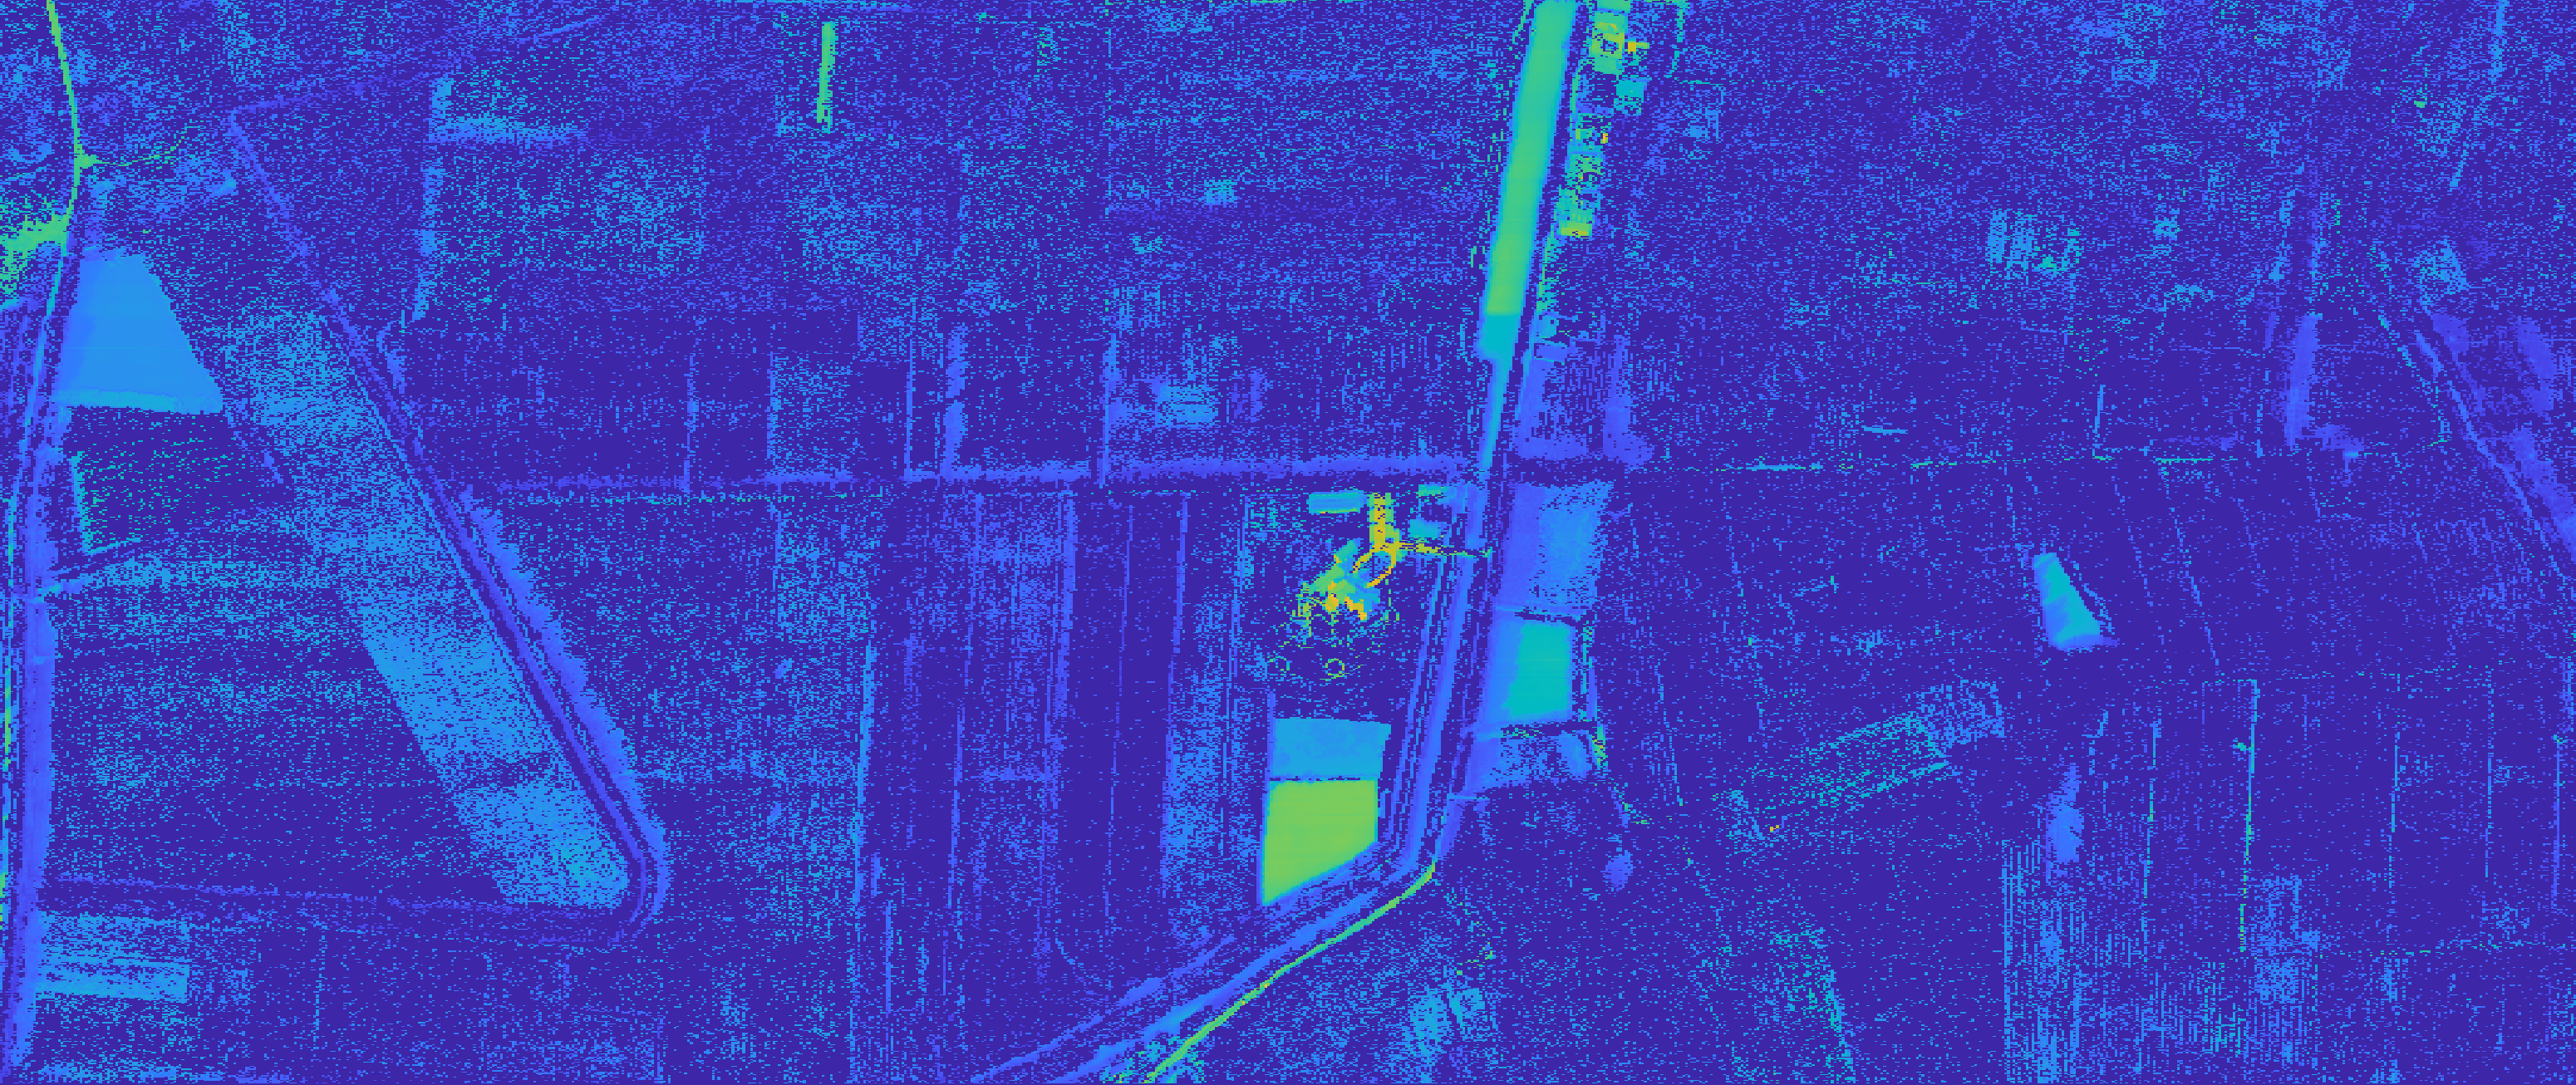
\includegraphics[width=0.485\linewidth]{xiongan-gcac_cr100.pdf}
        \label{fig_Result-Xiongan-gcc-cr0.01}
    }
    \subfloat[L1: $cr=10$]{
        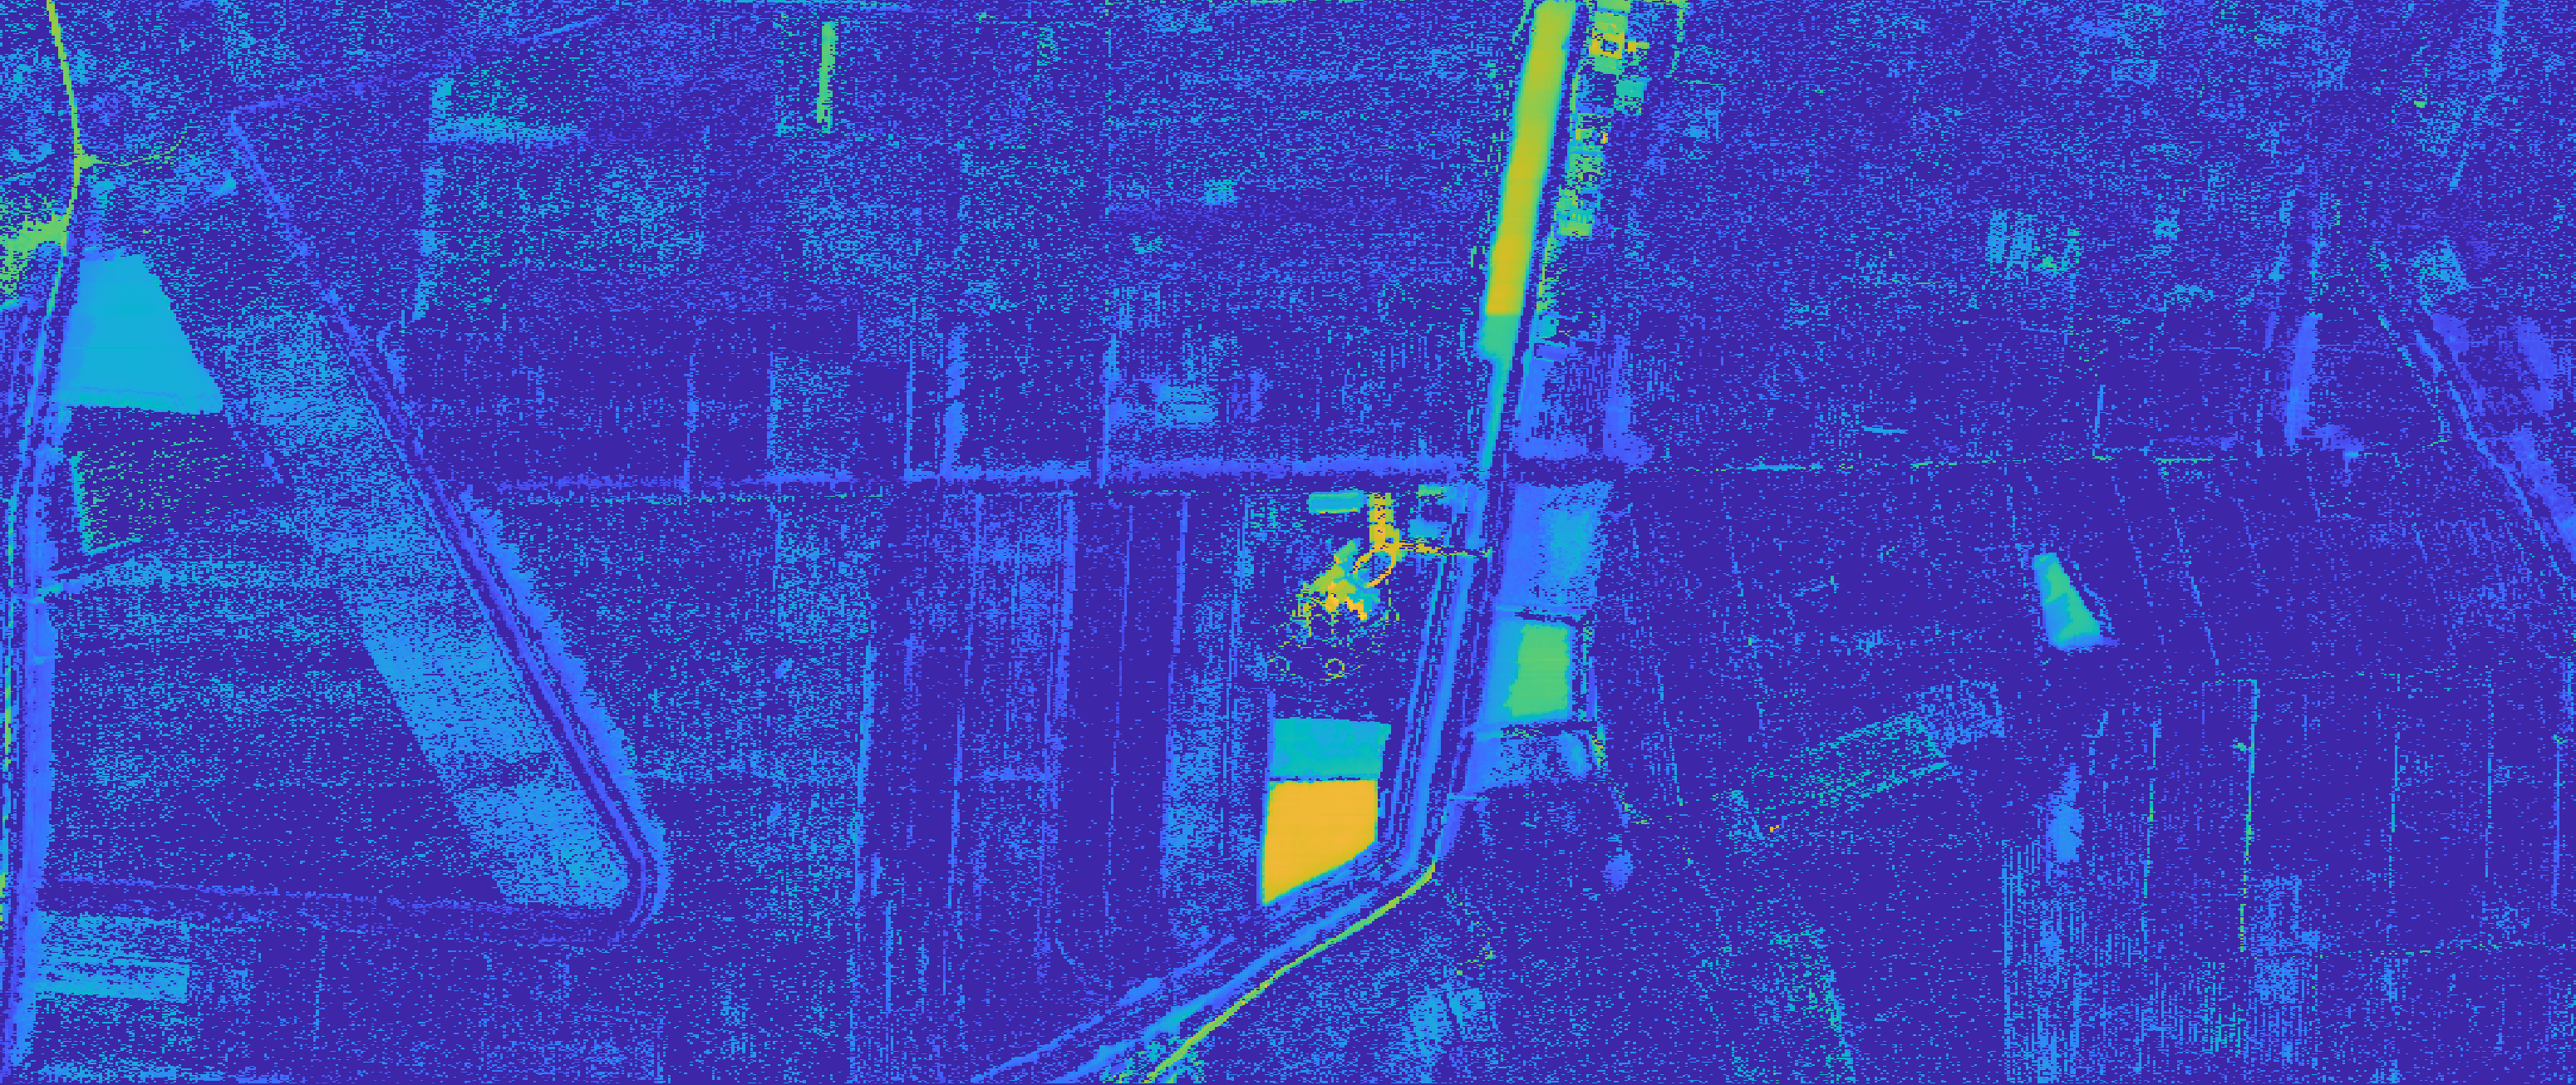
\includegraphics[width=0.485\linewidth]{xiongan-l1_cr10.pdf}
        \label{fig_Result-Xiongan-l1-cr0.1}
    } \\
    \subfloat[DGC: $cr=10$]{
        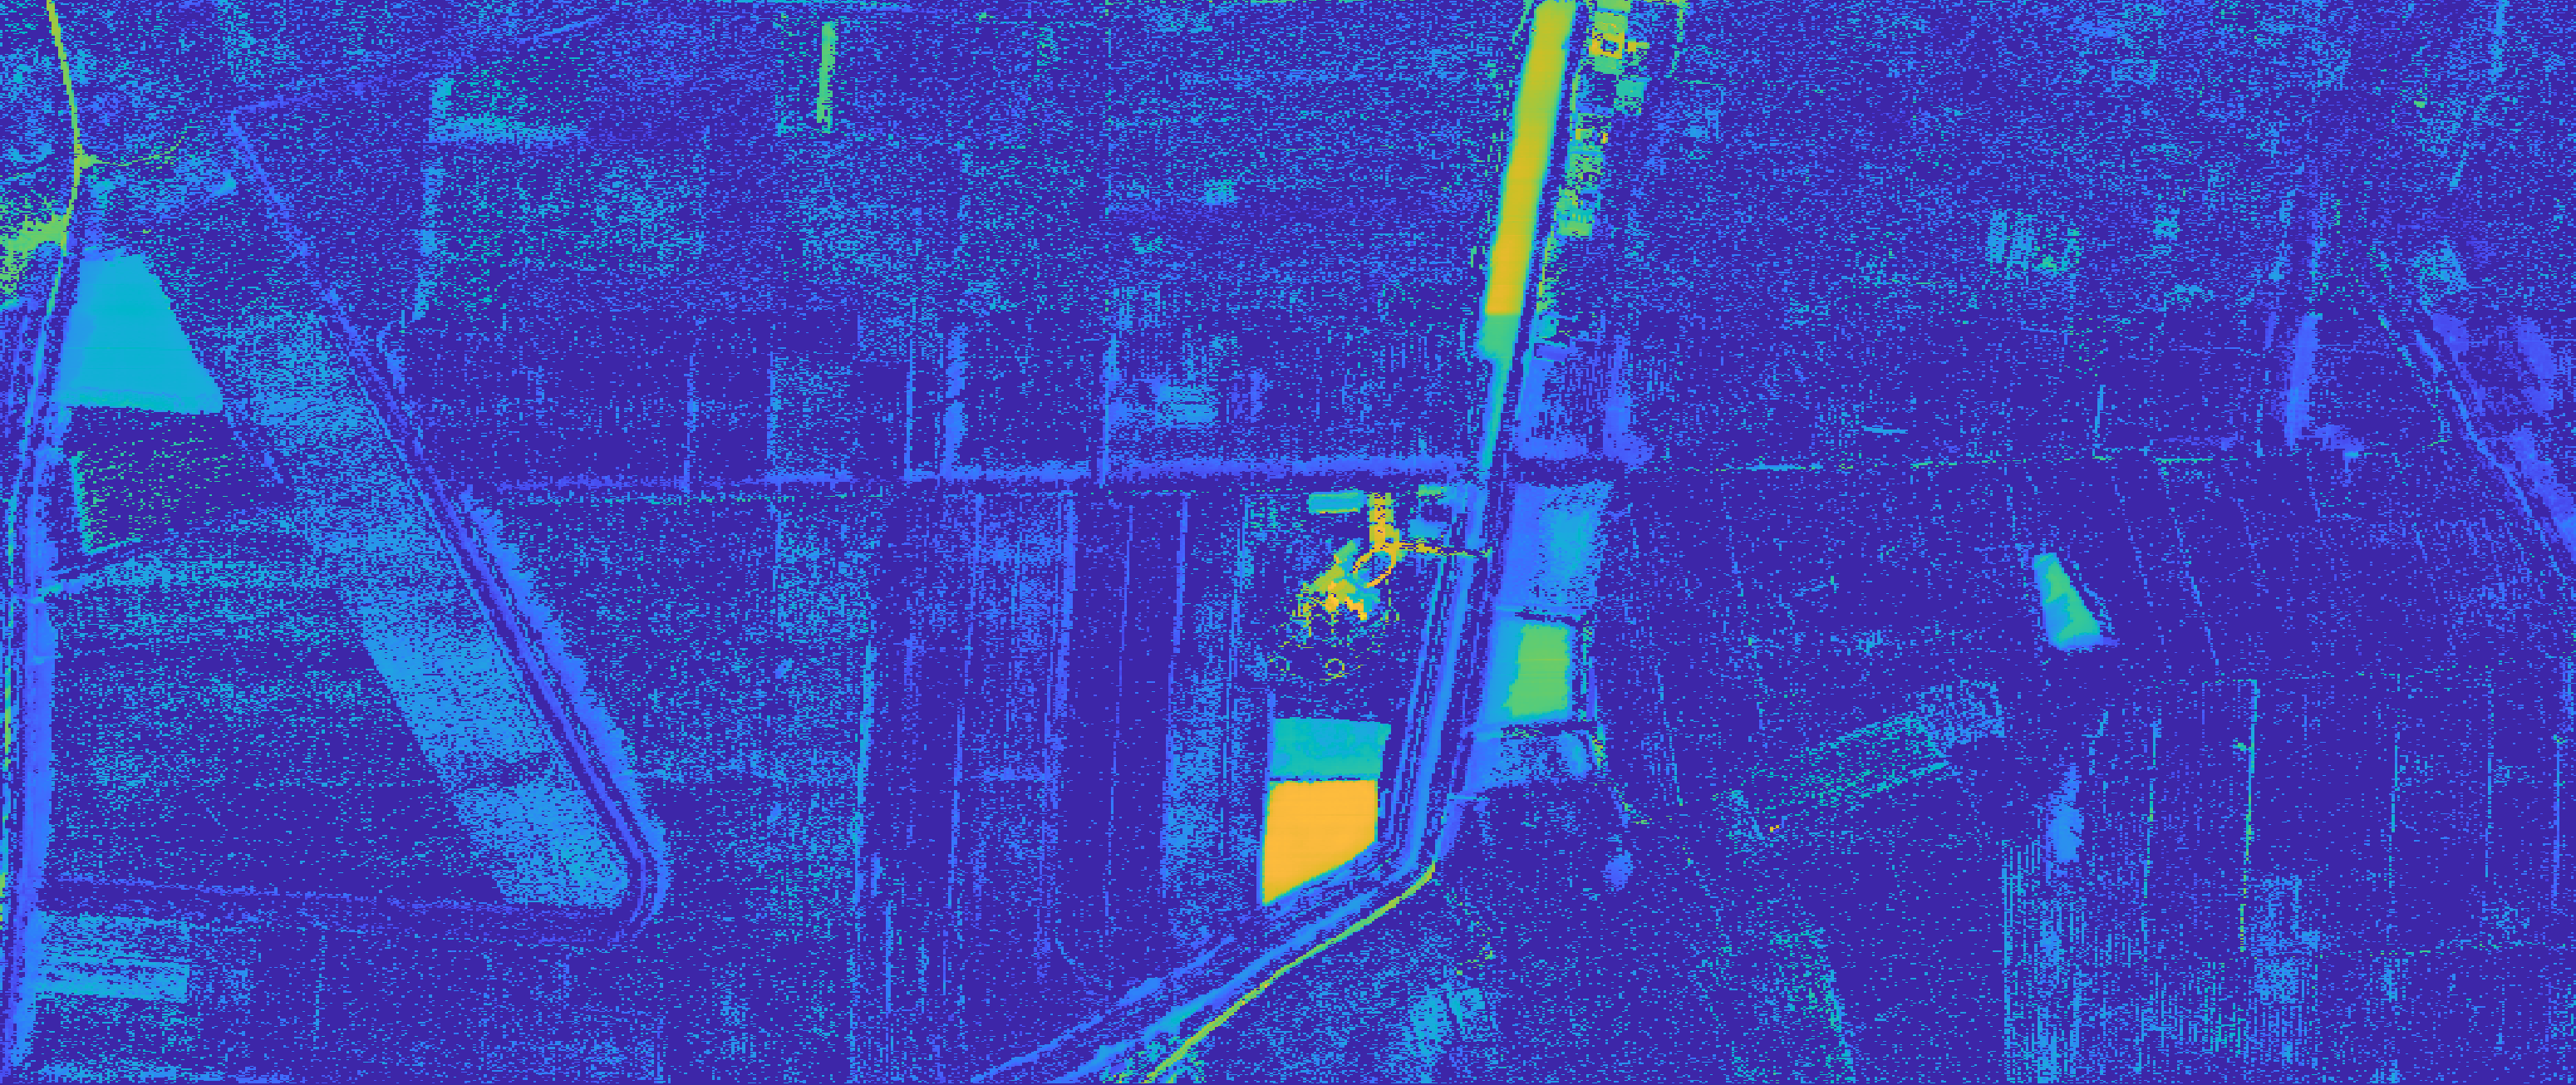
\includegraphics[width=0.485\linewidth]{xiongan-dgc_cr10.pdf}
        \label{fig_Result-Xiongan-dgc-cr0.1}
    }
    \subfloat[Top-k: $cr=10$]{
        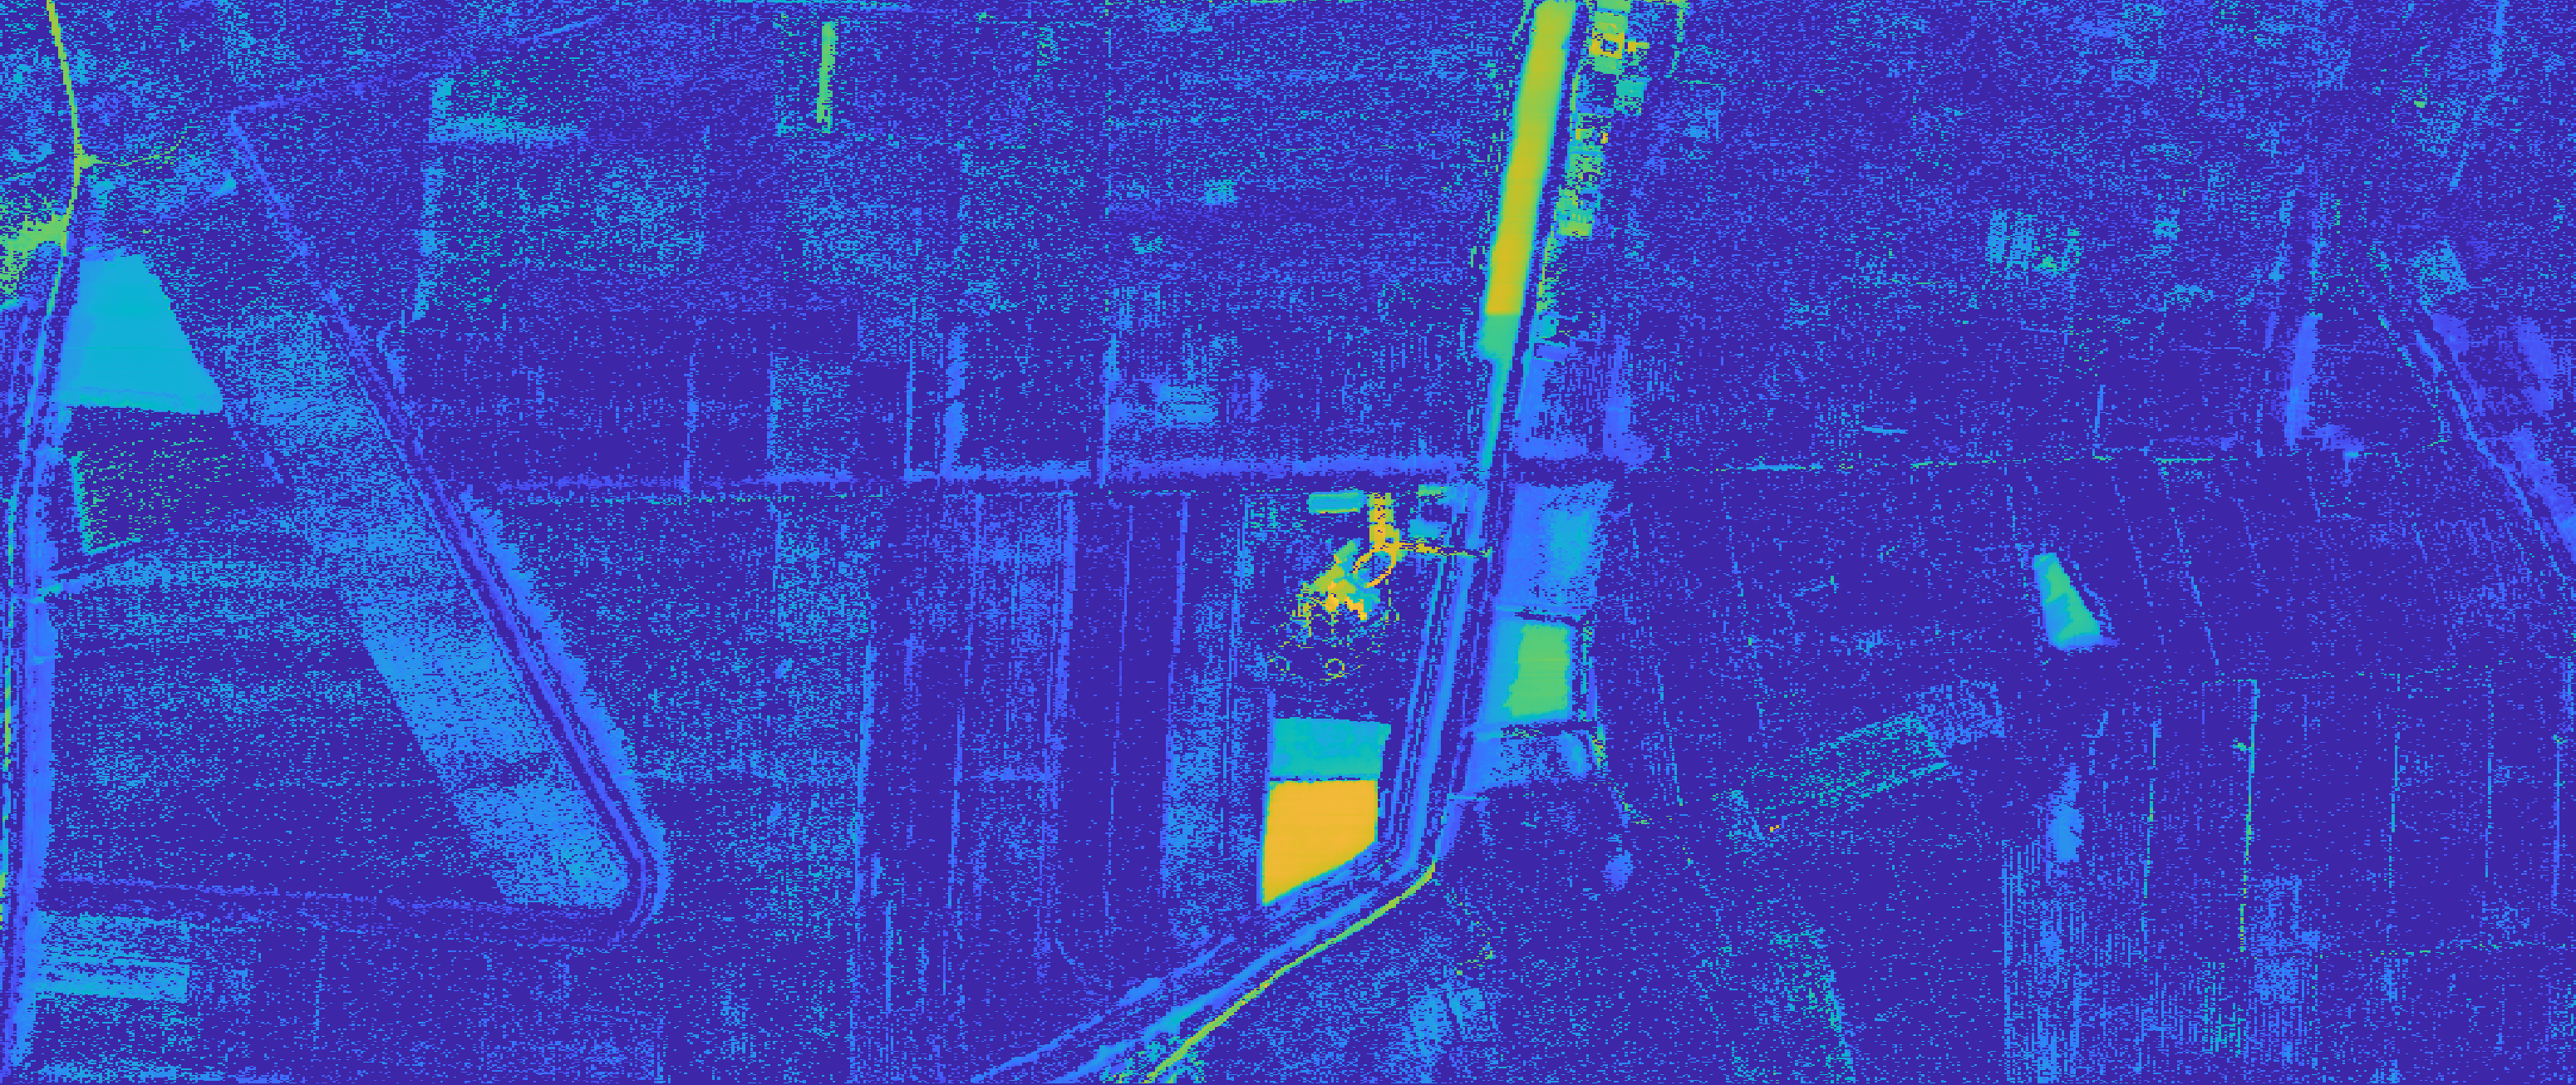
\includegraphics[width=0.485\linewidth]{xiongan-top-k_cr10.pdf}
        \label{fig_Result-Xiongan-top-k-cr0.1}
    }
    \caption{Xiongan数据集上,使用不同梯度压缩算法进行分布式训练的高光谱目标检测可视化结果}
    \label{fig_Result-Xiongan}
\end{figure}
%%%%%%%%%%%%%%%%%%%%%%%%%%%%%%%%%%%%%%%

通过图 \ref{fig_Result-AeroRIT} 以及图 \ref{fig_Result-Xiongan} 的效果进行对比,
我们可以清楚地看到,在相同的压缩比条件下,GCAC算法获取到的目标检测结果明显优于L1、DGC、Top-K等算法。
而当与Baseline进行对比时,可以发现在较小压缩比条件下,两者之间的差距非常小,目标都可以被很好地检测出来。
然而,通过图 \ref{fig_Result-AeroRIT} \subref{fig_Result-AeroRIT-gcc-cr0.1} 与图 \ref{fig_Result-AeroRIT} \subref{fig_Result-AeroRIT-gcc-cr0.01} 
以及图 \ref{fig_Result-Xiongan} \subref{fig_Result-Xiongan-gcc-cr0.1} 与
图 \ref{fig_Result-Xiongan} \subref{fig_Result-Xiongan-gcc-cr0.01} 的对比,
我们可以发现,当压缩比从10增大100时,GCAC算法并不能很好地适应这种变化,
从而导致检测效果不佳。这种情况出现的可能原因是:在实践中,由于我们为了加快计算梯度张量的质心位置,采用了“近似质心”进行代替,导致在采用保留下来的梯度进行模型训练时,梯度更新的方向与原优化方向有所偏差。


如图 \ref{fig_Result-AeroRIT}、\ref{fig_Result-Xiongan} 所示,采用了目标检测效果图来评估算法性能。
然而,这种评价方式由于主观性较强且不够全面,因此我们采用了更为客观和量化的评价指标,包括AUC、FPR等,以对算法的性能进行更深入的评估。
如表 \ref{tab_Result-gcc} 所示,总结了在不同数据集和不同压缩比的情况下,不同梯度压缩算法对网络模型检测性能的影响,并对本数据集中数值最大的AUC值以及最小的FPR值进行了加粗显示。

%%%%%%%%%%%%%%%%%%%%%%%%%%%%%%%%%%%%%%%
\renewcommand{\arraystretch}{1.3}
\begin{table*}[ht]
    \centering
    \begin{threeparttable}
        \caption{不同训练数据集上,使用不同梯度压缩算法进行分布式训练的HTD实验结果}
        \label{tab_Result-gcc}
        \begin{tabular}{c|c|c|c|c}
            \toprule
            \toprule
            数据集 & 梯度压缩算法 & 压缩比$cr$ & AUC($\%$) & FPR($\%$) \\
            \midrule
            AeroRIT & \multirow{2}{*}{Baseline} & \multirow{2}{*}{-} & \textbf{95.99} & \textbf{1.16} \\
            Xiongan New Aera(Matiwan Village) &  &  & \textbf{94.10} & 7.93 \\
            \midrule
            \multirow{7}{*}{AeroRIT} & \multirow{4}{*}{GCC} & 10$\times$ & \textbf{95.99} & 1.18 \\
             &  & 30$\times$ & 95.08 & 1.35 \\
             &  & 50$\times$ & 93.28 & 2.15 \\
             &  & 100$\times$ & 87.28 & 5.04 \\
             & L1 & 10$\times$ & 83.94 & 6.67 \\
             & DGC\cite{lin2017deep} & 10$\times$ & 95.23 & 1.58 \\
             & Top-K\cite{aji2017sparse} & 10$\times$ & 93.38 & 2.36 \\
            \midrule
            \multirow{7}{*}{Xiongan New Aera(Matiwan Village)} & \multirow{4}{*}{GCC} & 10$\times$ & \textbf{94.10} & 7.94 \\
             &  & 30$\times$ & 93.35 & \textbf{7.50} \\
             &  & 50$\times$ & 92.09 & 7.67 \\
             &  & 100$\times$ & 89.41 & 11.31 \\
             & L1 & 10$\times$ & 89.63 & 10.67 \\
             & DGC\cite{lin2017deep} & 10$\times$ & 93.63 & 7.78 \\
             & Top-K\cite{aji2017sparse} & 10$\times$ & 93.38 & 8.36 \\
            \bottomrule
            \bottomrule
        \end{tabular}
    \end{threeparttable}
\end{table*}
%%%%%%%%%%%%%%%%%%%%%%%%%%%%%%%%%%%%%%%

从表 \ref{tab_Result-gcc} 中的AUC值可以看出,本章所提出的GCAC算法在大规模遥感数据集上的表现非常具有竞争力,甚至已然超过DGC等先进的梯度压缩算法。
无论是在AeroRIT还是Xiongan New Area(Matiwan Village)遥感数据集上,
当压缩比为10时,GCAC算法都实现了无损压缩的效果,即AUC值与Baseline表现相同,同时明显优于其他梯度压缩算法。
另外,通过表 \ref{tab_Result-gcc} 中的FPR值可以看出,使用GCAC算法时,FPR值与Baseline十分接近,这说明在分布式训练场景中应用GCAC算法并没有对网络模型的虚警率产生较大影响。
然而,需要注意的是,由于GCAC算法在实践过程中采用了“近似质心”的计算加速技术,因此在面对大压缩比时,GCAC算法的表现仍有较大的提升空间。
上述的高光谱目标检测任务的实验表明,本章提出的基于近似质心的梯度压缩算法在小压缩比的情况下表现优异,但在大压缩比的情况下,网络模型的性能有较大的下降,成为了该算法的一个不足之处。

%%%%%%%%%%%%%%%%%%%%%%%%%%%%%%%%%%%%%%%
\begin{figure}[!t]
    \centering
    \subfloat[VGGNet-16 Top-1 Test Acc.]{
        % \includegraphics[width=0.488\linewidth]{vgg16-chap-3-0-acc.pdf}
        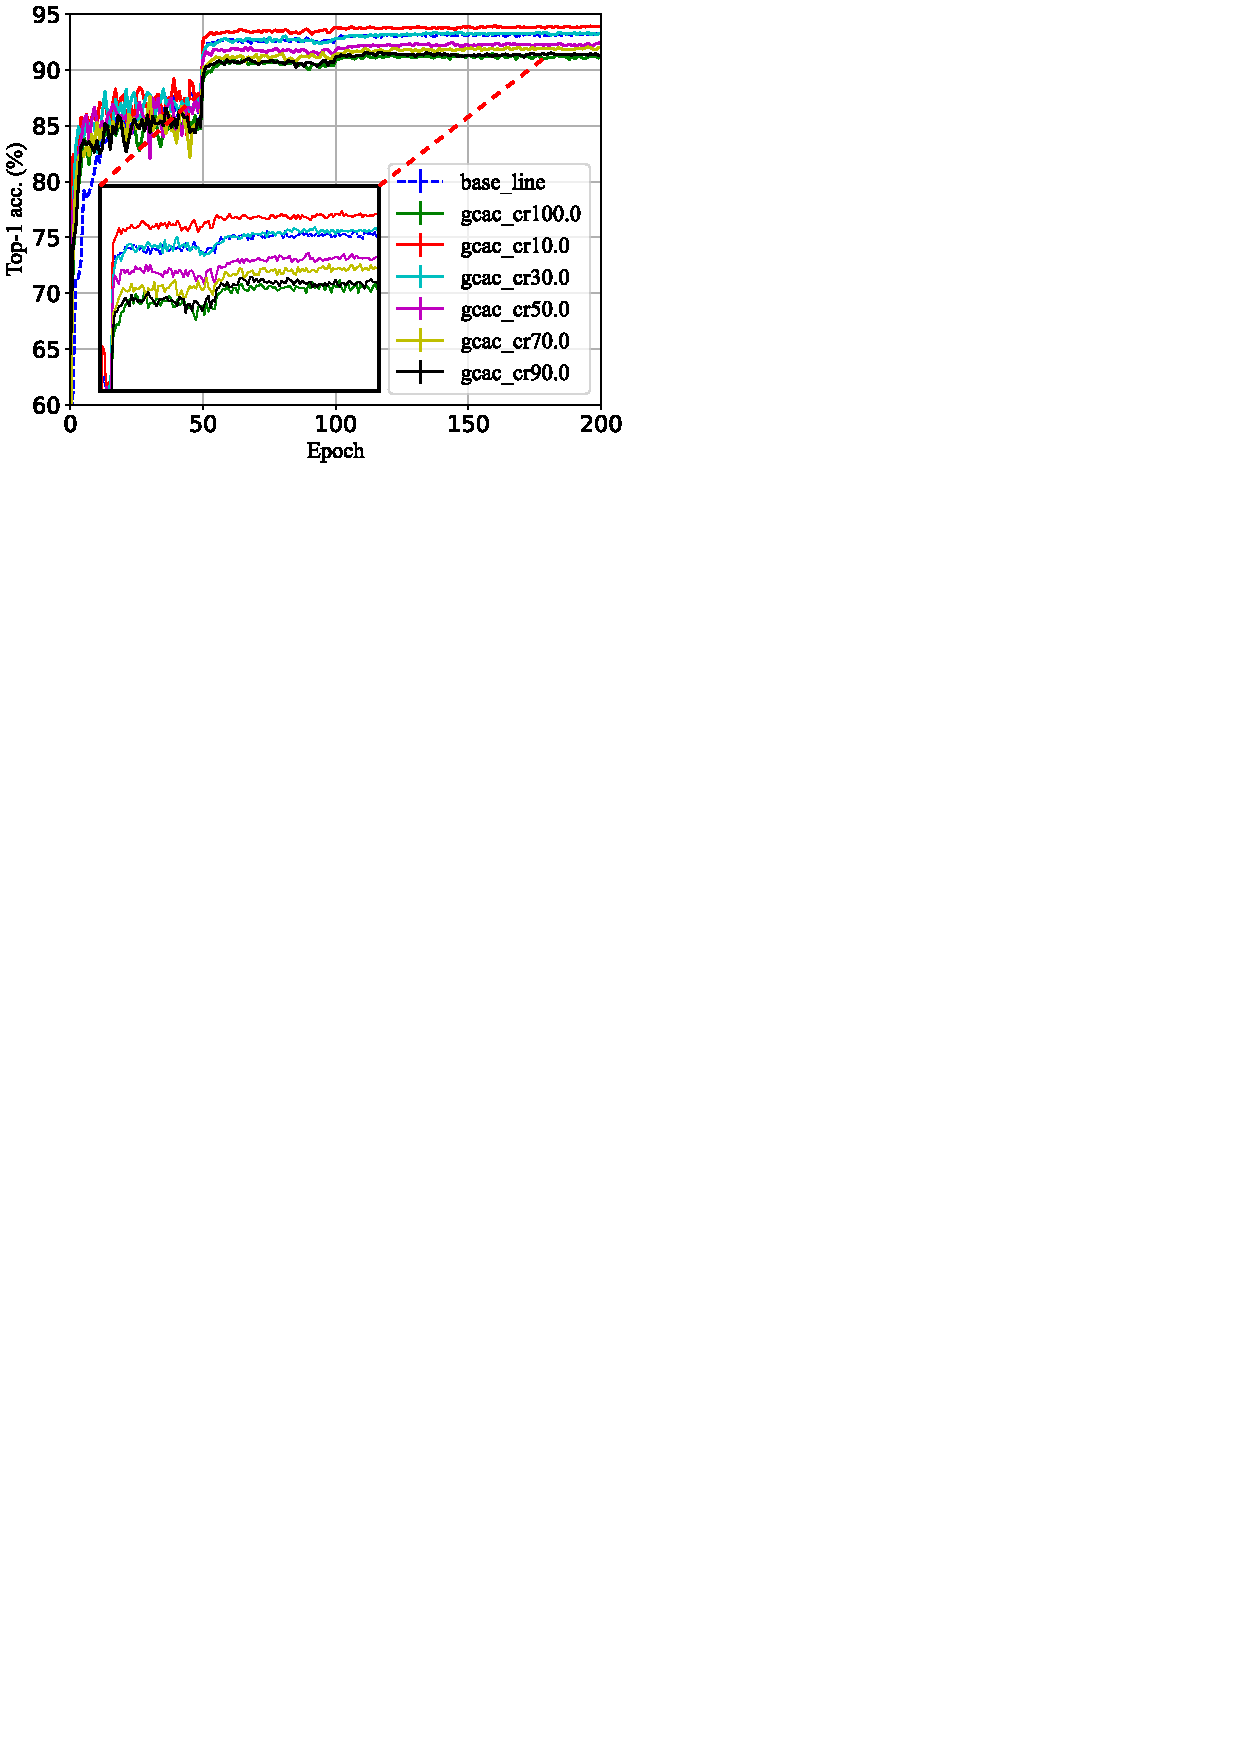
\includegraphics[width=0.488\linewidth]{vgg16-chap-3-0-acc-v2.pdf}
        \label{fig_Result-vgg16-acc}
    }
    \subfloat[VGGNet-16 Train loss]{
        % \includegraphics[width=0.488\linewidth]{vgg16-chap-3-0-loss.pdf}
        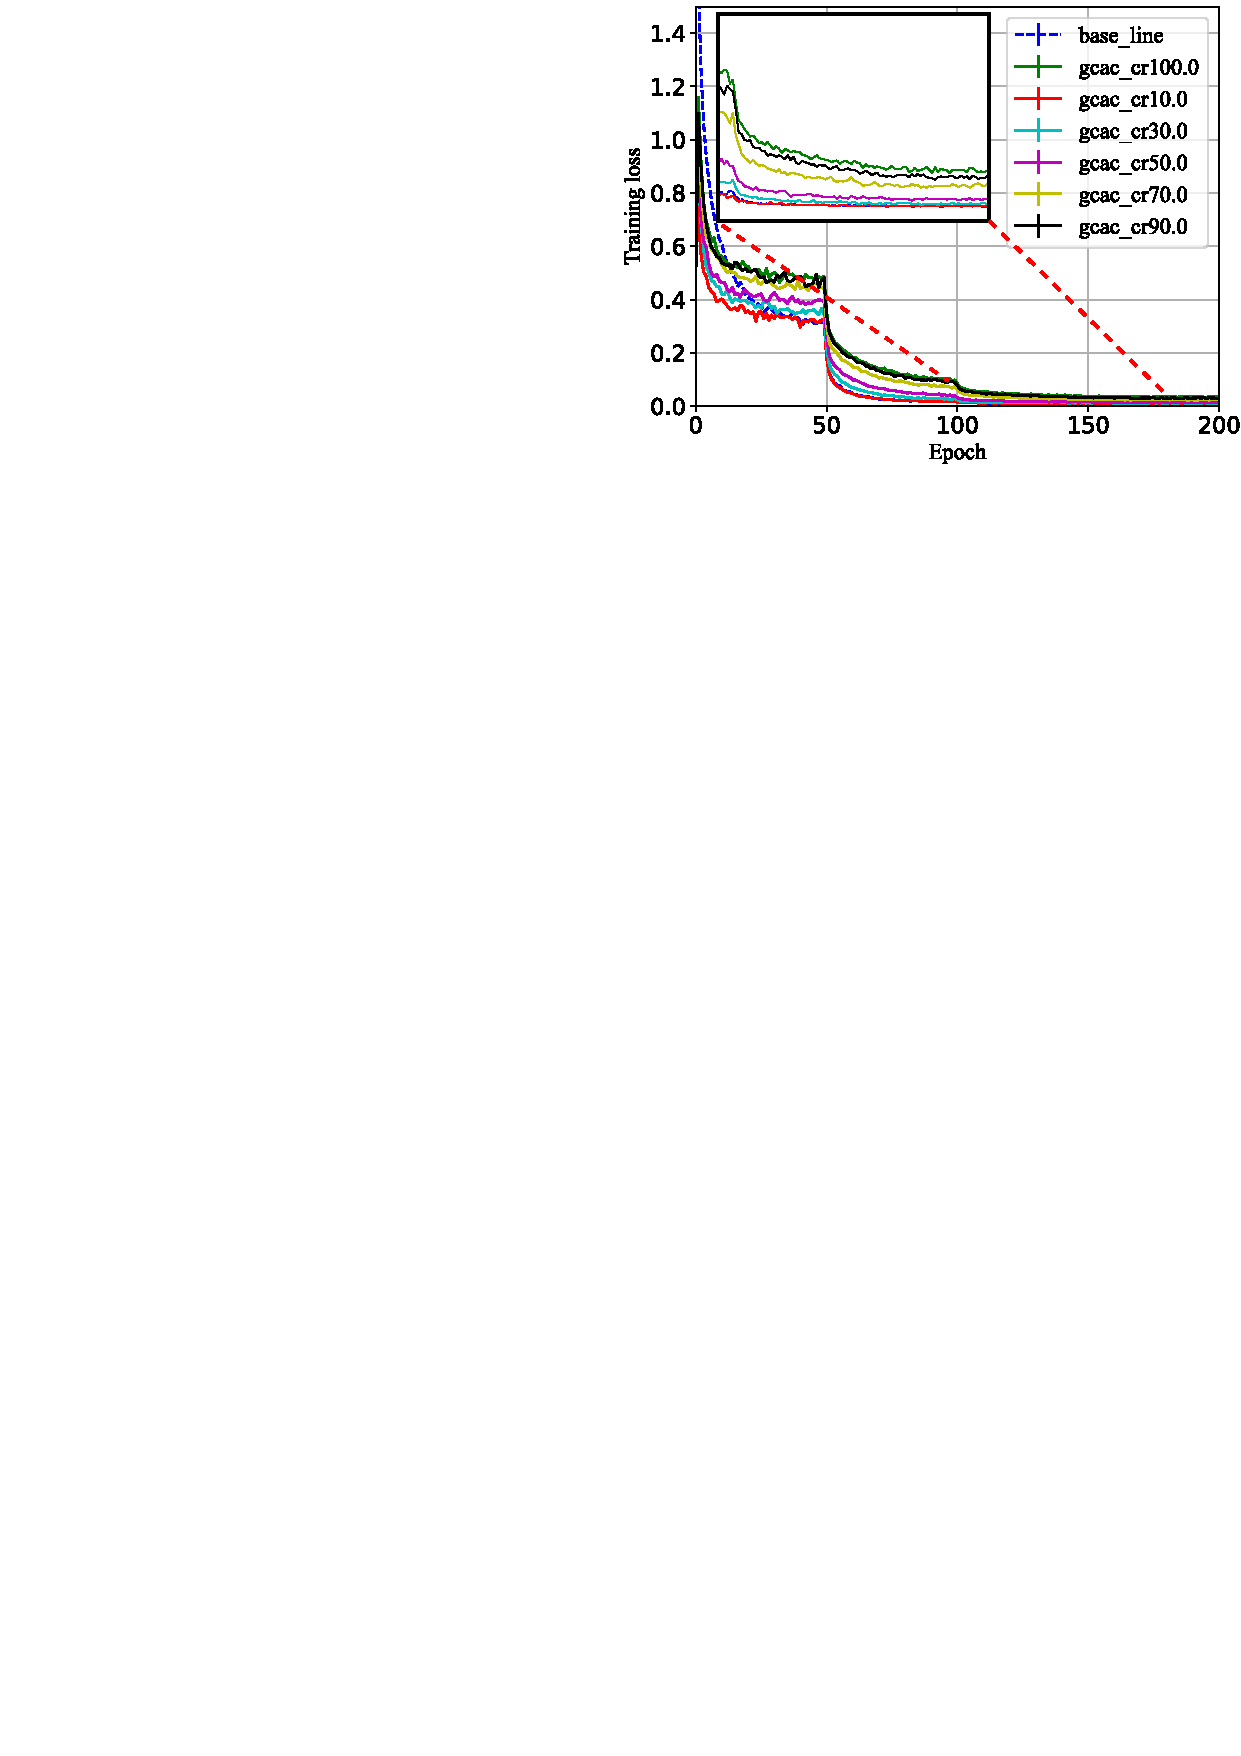
\includegraphics[width=0.488\linewidth]{vgg16-chap-3-0-loss-v2.pdf}
        \label{fig_Result-vgg16-loss}
    } \\
    \subfloat[ResNet-56 Top-1 Test Acc.]{
        % \includegraphics[width=0.488\linewidth]{resnet56-chap-3-0-acc.pdf}
        \includegraphics[width=0.488\linewidth]{resnet56-chap-3-0-acc-v2.pdf}
        \label{fig_Result-resnet56-acc}
    }
    \subfloat[ResNet-56 Train loss]{
        % \includegraphics[width=0.488\linewidth]{resnet56-chap-3-0-loss.pdf}
        \includegraphics[width=0.488\linewidth]{resnet56-chap-3-0-loss-v2.pdf}
        \label{fig_Result-resnet56-loss}
    } \\
    \subfloat[ResNet-110 Top-1 Test Acc.]{
        % \includegraphics[width=0.488\linewidth]{resnet110-chap-3-0-acc.pdf}
        \includegraphics[width=0.488\linewidth]{resnet110-chap-3-0-acc-v2.pdf}
        \label{fig_Result-resnet110-acc}
    }
    \subfloat[ResNet-110 Train loss]{
        % \includegraphics[width=0.488\linewidth]{resnet110-chap-3-0-loss.pdf}
        \includegraphics[width=0.488\linewidth]{resnet110-chap-3-0-loss-v2.pdf}
        \label{fig_Result-resnet110-loss}
    } \\
    \caption{CIFAR10数据集上,不同网络模型采用GCAC算法进行分布式训练的$acc_{1}$与loss曲线}
    \label{fig_Result-gcc}
\end{figure}
%%%%%%%%%%%%%%%%%%%%%%%%%%%%%%%%%%%%%%%


\subsection{图像分类实验结果分析}
%%%%%%%%%%%%%%%%%%%%%%%%%%%%%%%%%%%%%%%
\begin{figure}[!t]
    \centering
    \subfloat[VGGNet-16 Top-1 Test Acc.]{
        % \includegraphics[width=0.488\linewidth]{vgg16-chap-3-1-acc.pdf}
        \includegraphics[width=0.488\linewidth]{vgg16-chap-3-1-acc-v2.pdf}
        \label{fig_Result-vgg16-acc-contrast}
    } 
    \subfloat[VGGNet-16 Train loss]{
        % \includegraphics[width=0.488\linewidth]{vgg16-chap-3-1-loss.pdf}
        \includegraphics[width=0.488\linewidth]{vgg16-chap-3-1-loss-v2.pdf}
        \label{fig_Result-vgg16-loss-contrast}
    } \\
    \subfloat[ResNet-56 Top-1 Test Acc.]{
        % \includegraphics[width=0.488\linewidth]{resnet56-chap-3-1-acc.pdf}
        \includegraphics[width=0.488\linewidth]{resnet56-chap-3-1-acc-v2.pdf}
        \label{fig_Result-resnet56-acc-contrast}
    }
    \subfloat[ResNet-56 Train loss]{
        % \includegraphics[width=0.488\linewidth]{resnet56-chap-3-1-loss.pdf}
        \includegraphics[width=0.488\linewidth]{resnet56-chap-3-1-loss-v2.pdf}
        \label{fig_Result-resnet56-loss-contrast}
    } \\
    \subfloat[ResNet-110 Top-1 Test Acc.]{
        % \includegraphics[width=0.488\linewidth]{resnet110-chap-3-1-acc.pdf}
        \includegraphics[width=0.488\linewidth]{resnet110-chap-3-1-acc-v2.pdf}
        \label{fig_Result-resnet110-acc-contrast}
    }
    \subfloat[ResNet-110 Train loss]{
        % \includegraphics[width=0.488\linewidth]{resnet110-chap-3-1-loss.pdf}
        \includegraphics[width=0.488\linewidth]{resnet110-chap-3-1-loss-v2.pdf}
        \label{fig_Result-resnet110-loss-contrast}
    } \\
    \caption{CIFAR10数据集上,不同网络模型采用不同梯度压缩算法进行分布式训练的$acc_{1}$与loss曲线}
    \label{fig_Result-gcc-contrast}
\end{figure}
%%%%%%%%%%%%%%%%%%%%%%%%%%%%%%%%%%%%%%%

为了充分验证所提出的基于近似质心的梯度压缩算法的泛化能力,我们将其应用到自然图像分类这一下游任务中。
第 \ref{sec_EnvironmentAndHyperParameterSet} 小节详细描述了本任务所涉及到的模型部署环境、网络模型选择以及模型超参数设置等相关内容。

图 \ref{fig_Result-gcc} 展示了在CIFAR10数据集上,使用GCAC算法进行分布式训练不同规模的网络模型(VGGNet-16、ResNet-56以及ResNet-110)的测试精度和训练损失曲线。
其中,第一行中图 \ref{fig_Result-gcc} \subref{fig_Result-vgg16-acc}、
图 \ref{fig_Result-gcc} \subref{fig_Result-vgg16-loss},
第二行中图 \ref{fig_Result-gcc} \subref{fig_Result-resnet56-acc}、
图 \ref{fig_Result-gcc} \subref{fig_Result-resnet56-loss},
第三行中图 \ref{fig_Result-gcc} \subref{fig_Result-resnet110-acc}、
图 \ref{fig_Result-gcc} \subref{fig_Result-resnet110-loss} 
分别展示了不压缩(Baseline)以及不同压缩比的情况下,VGGNet-16、ResNet-56以及ResNet-110三个网络模型的测试精度和训练损失曲线。
可以看出,无论是VGGNet还是ResNet网络模型,在分布式训练过程中采用GCAC算法时,其收敛速度都比于Baseline更快。
此外,当压缩比较小时,网络模型的性能表现甚至超过了Baseline,这表明在梯度张量中存在一部分对模型优化起到反作用的梯度,因此,在整个分布式训练过程中,针对不同的目标选择合适的算法进行梯度稀疏化是相当重要的。
需要注意的是,在压缩比较大(例如100)的情况下,采用GCAC算法进行分布式训练的网络模型性能表现有所下降,这中现象归因于“近似质心”的加速计算技术。


如图 \ref{fig_Result-gcc-contrast} 所示,在CIFAR10数据集上,对不同网络模型(VGGNet-16、ResNet-56以及ResNet-110)采用了不同的梯度压缩算法进行分布式训练,
并展示了其测试精度以及训练损失曲线。
需要注意的是,该图仅选取了两个具有代表性的压缩比(10和100)进行比较。
与采用L1-范数为梯度度量梯度压缩算法相比,无论是从收敛速度还是网络模型性能表现来看,GCAC算法的表现更好,并且当网络模型收敛后,分布式训练的loss值更小。
因此,可以得出结论,GCAC算法可以在保证网络模型精度的同时,还可以大幅提高分布式的训练效率。
 

如表 \ref*{tab_Result-gcc-CIFAR10} 展示了在CIFAR10数据集上,不同网络模型采用不同梯度压缩算法进行分布式训练的$acc_{1}$与损失loss收敛值。
正如图 \ref*{fig_Result-gcc} 与图 \ref*{fig_Result-gcc-contrast} 所展示的,
当分布式训练过程中的梯度压缩比$cr$较小时,GCAC算法的表现非常出色。
尤其面向较大规模的网络模型时,该算法训练出来模型Top-1精度甚至超过了DGC算法。
与其他梯度压缩算法对比,采用GCAC算法的网络模型损失loss收敛值更接近于零,这表明该网络模型与训练数据集的贴合度更高。
然而,该表格也反映出,本章提出的GCAC算法在面对大压缩比的挑战时,表现不尽如人意,导致网络模型的性能下降严重,该现象在理论上归因于“近似质心”的加速计算技术。

%%%%%%%%%%%%%%%%%%%%%%%%%%%%%%%%%%%%%%%
\renewcommand{\arraystretch}{1.3}
\begin{table*}[ht]
    \centering
    \begin{threeparttable}
        \caption{CIFAR10数据集上,GCAC与其他算法的分布式训练$acc_{1}$与loss收敛值}
        \label{tab_Result-gcc-CIFAR10}
        \begin{tabular}{c|c|c|c|c}
            \toprule
            \toprule
            网络模型 & 梯度压缩算法 & 梯度压缩比$cr$ & Top-1 Acc. ($\%$)& loss收敛值 \\
            \midrule
            \multirow{6}{*}{VGGNet-16} & Baseline & - & 93.17 & 0.0105 \\
                & GCAC   & 10$\times$ / 100$\times$ & \textbf{93.28} / 90.84 & 0.0101 / 0.0359 \\
                & L1     & 10$\times$ / 100$\times$ & 91.46 / 90.32 & 0.0118 / 0.0140 \\
                & Top-K  & 10$\times$ / 100$\times$ & 92.45 / 91.48 & 0.0141 / 0.0291 \\
                & DGC    & 10$\times$ / 100$\times$ & 93.24 / 92.04 & \textbf{0.0100} / 0.0123 \\
                & Random & 10$\times$ / 100$\times$ & 90.69 / 75.06 & 0.0378 / 0.9185 \\
            \midrule
            \multirow{6}{*}{ResNet-56} & Baseline & - & \textbf{93.07} & \textbf{0.0211} \\
                & GCAC   & 10$\times$ / 100$\times$ & 92.23 / 90.89 & 0.0334 / 0.0745 \\
                & L1     & 10$\times$ / 100$\times$ & 91.30 / 89.51 & 0.0354 / 0.0816 \\
                & Top-K  & 10$\times$ / 100$\times$ & 91.41 / 90.77 & 0.0657 / 0.0811\\
                & DGC    & 10$\times$ / 100$\times$ & 92.52 / 91.08 & 0.0243 / 0.0589 \\
                & Random & 10$\times$ / 100$\times$ & 88.84 / 75.53 & 0.2631 / 0.9435 \\
            \midrule
            \multirow{6}{*}{ResNet-110} & Baseline & - & 93.24 & 0.0116 \\
                & GCAC   & 10$\times$ / 100$\times$ & \textbf{94.07} / 91.14 & \textbf{0.0110} / 0.0224 \\
                & L1     & 10$\times$ / 100$\times$ & 92.38 / 91.08 & 0.0252 / 0.0372 \\
                & Top-K  & 10$\times$ / 100$\times$ & 91.87 / 91.03 & 0.0265 / 0.338 \\
                & DGC    & 10$\times$ / 100$\times$ & 93.20 / 91.65 & 0.0113 / 0.0174 \\
                & Random & 10$\times$ / 100$\times$ & 91.41 / 84.61 & 0.0421 / 0.5033 \\
            \bottomrule
            \bottomrule
        \end{tabular}
    \end{threeparttable}
\end{table*}
%%%%%%%%%%%%%%%%%%%%%%%%%%%%%%%%%%%%%%%


\subsection{耗时分析}
分布式训练过程中采用梯度压缩技术的目的有两个:1)减小网络拓扑中各Worker之间通信的数据量;
2)缩短节点间的通信时间。
显然,梯度压缩算法可以轻松实现第一个目标,而个缩短通信时间不仅与节点数量有关,
也与网络通信内容数据量息息相关,即网络通信中节点数量越多、通信内容数据量越大,通信时间越长。
GCAC算法旨在减少通信内容数据量,在控制网络节点数量不变的情况下,
表 \ref{tab_Result-time-contrast} 展示了不进行梯度压缩与采用梯度压缩网络模型训练相关时长统计,包括每次迭代平均用时、梯度压缩平均用时及其占比。

%%%%%%%%%%%%%%%%%%%%%%%%%%%%%%%%%%%%%%%
\renewcommand{\arraystretch}{1.3}
\begin{table*}[ht]
    \centering
    \begin{threeparttable}
        \caption{CIFAR10数据集上,不同网络模型采用不同梯度压缩算法的耗时比较}
        \label{tab_Result-time-contrast}
        \begin{tabular}{c|c|c|c|c}
            \toprule
            \toprule
            \multirow{2}{*}{网络模型} & \multirow{2}{*}{梯度压缩算法} & 迭代平均用时 & 梯度压缩平均 & 梯度压缩用时 \\
            & & (毫秒) & 用时(毫秒)& 占比($\%$) \\
            \midrule
            \multirow{5}{*}{VGGNet-16} & Baseline & 640.99 & - & - \\
                  & GCAC & 828.70 & 348.78 & 42.09 \\
                  & L1 & 828.17 & \textbf{347.18} & \textbf{41.92} \\
                  & Top-K & 862.27 & 418.46 & 48.53 \\
                  & DGC & 1375.42 & 906.56 & 65.91 \\
            \midrule
            \multirow{5}{*}{ResNet-56} & Baseline & 157.33 & - & - \\
                  & GCAC & 333.28 & \textbf{230.15} & 69.06 \\
                  & L1 & 335.80 & 230.38 & \textbf{68.61} \\
                  & Top-K & 395.59 & 277.66 & 70.19 \\
                  & DGC & 557.86 & 460.00 & 82.46 \\
            \midrule
            \multirow{5}{*}{ResNet-110} & Baseline & 289.08 & - & - \\
                  & GCAC & 629.85 & \textbf{382.52} & \textbf{60.73} \\
                  & L1 & 612.90 & 397.79 & 64.90 \\
                  & Top-K & 653.27 & 494.00 & 75.62 \\
                  & DGC & 1067.71 & 866.94 & 81.20 \\
            \bottomrule
            \bottomrule
        \end{tabular}
    \end{threeparttable}
\end{table*}
%%%%%%%%%%%%%%%%%%%%%%%%%%%%%%%%%%%%%%%

根据该表可见,本文提出的GCAC算法与L1算法的梯度压缩平均用时接近,这主要得益于采用了“近似质心”的加速计算技术以及GPU并行计算。
与Top-K梯度压缩算法对比,当网络模型参数量较大时(如VGGNet-16、ResNet-110),GCAC算法进行梯度压缩平均耗时占比优势更加明显,仅占用总迭代时长的$6\%$左右。
相较于DGC算法,GCAC算法梯度压缩用时占比更小,主要是因为DGC采用的延迟通信操作被计入了梯度压缩用时。
更重要的是,无论是小规模(ResNet-56)还是大规模网络模型(VGGNet-16、ResNet-110),
GCAC算法只需要花费少量时间对梯度进行压缩操作,就可以大幅减少各节点之间的通信数据量,
进而大幅缩减通信时间。
例如,在CIFAR10数据集上,大规模网络模型VGGNet-16进行分布式训练过程中,采用GCAC算法进行梯度压缩操作,只需花费原迭代平均用时的0.29倍。


\section{本章小结}
\label{sec_Summary-3}
为了降低分布式训练过程中各Worker之间的通信数据量,本章提出一种新的梯度压缩算法,即基于近似质心的梯度压缩算法(Gradient Compression via Approximate Centroid,GCAC)。
该算法利用网络模型局部梯度张量的质心特性,选择部分梯度代替全局梯度进行通信,旨在保证网络模型性能的情况下提高分布式训练速度。
算法的核心思路是:网络拓扑中每个Worker首先获取本地的局部网络模型梯度张量,
然后根据“近似质心”的加速计算技术计算每一个梯度与“近似质心”之间的距离,并基于该距离进行梯度排序,随后根据预设压缩比选择相应数量的梯度索引,据此得到待传输梯度,最后进行梯度更新并进入下一次迭代。
我们在多个下游任务上进行了GCAC算法的验证工作,并与现有梯度压缩算法进行了对比。
实验结果表明,基于近似质心的梯度压缩算法具有很强的通用性,可以适应高光谱目标检测、自然图像分类等不同类型的任务。
同时,GCAC算法只需在各Worker通信之前花费少量时间进行梯度压缩操作,从而缓解了整个分布式训练的瓶颈难题,大大提高了网络模型训练速度。
另外,实验还发现GCAC算法在压缩比较小时可以完美应用到大数据大模型场景下,
但在大压缩比场景下会导致网络模型性能下降较多,是该算法的一个不足之处。



%%%%%%%%%%%%%%%%%%%%%%%%%%%%%%%%%%%%%%%%%%%%%%%%%%%%%%%%%%%
%%%%%%%%%%%%%%%%%%%%%%%%%%%%%%%%%%%%%%%%%%%%%%%%%%%%%%%%%%%
% \chapter{基于$k$-互异近邻的梯度压缩算法}
\chapter{基于\texorpdfstring{$k$}.-互异近邻的梯度压缩算法}
\section{引言}
% 第\ref{sec_chapter-3}章节详细介绍了基于近似质心的梯度压缩算法-GCAC。
在大规模数据集、高复杂度网络模型场景下,与现有一些梯度压缩算法(如Top-K、DGC等)相比,第\ref{sec_chapter-3}章提出的GCAC算法在最终网络模型的性能表现、梯度压缩平均耗时等方面取得了一定的优势。
但在大压缩比的情况下,采用GCAC算法的网络模型最终性能表现下降较多,是该算法的一个不足之处。
因此,发现在大压缩比场景下GCAC算法表现不足的难题后,本章进一步思考、分析梯度张量的相关特性,
提出基于$k$-互异近邻的梯度压缩算法(Gradient Compression based on $k$-Reciprocal Nearest neighbors,$k$-RNGC)。

$k$-RNGC算法实现了独立计算感知梯度重要性的测量方法,根据梯度测量结果对梯度进行排序和预选择,
同时还设计了$k$-互异近邻梯度选择方案,从推荐的梯度中选择出待保留的梯度。
另外,为了提高大压缩比场景下的算法表现,引入动量修正和预热训练两大核心组件,克服了通信频率降低导致的梯度陈旧问题,保证稀疏化网络模型的性能表现。

本章首先在第 \ref{sec_k-RNGC} 小节介绍$k$-RNGC算法的核心内容,包括计算感知算法、$k$-互异近邻梯度选择算法、动量修正、预热训练以及整体框架等。
接着,第 \ref{sec_chapter4-Exper} 小节介绍高光谱目标检测和自然图像分类两个下游任务上的验证实验以及结果分析,主要包括组件分析、耗时分析以及对比实验。
最后,第 \ref{sec_chapter4-Summary} 小节总结本章主要的研究工作。

\section{基于\texorpdfstring{$k$}.-互异近邻的梯度压缩算法}
\label{sec_k-RNGC}
\subsection{计算感知获取局部梯度压缩比}
%%%%%%%%%%%%%%%%%%%%%%%%%%%%%%%%%%%%%%%
\begin{figure}[ht]
    \centering
    \includegraphics[width=0.90\textwidth]{k-RNGC.pdf}
    \caption{通过计算感知算法以获取网络模型局部压缩比原理图}
    \label{fig_k-RNGC-global-rank}
\end{figure}
%%%%%%%%%%%%%%%%%%%%%%%%%%%%%%%%%%%%%%%

假设给定全局梯度压缩比为$cr$,全局排序的目标则是通过假定裁剪掉某些排名靠后的梯度,
使得裁剪后的梯度张量满足压缩比条件,然后根据保留梯度反向推导出其在网络模型中所处的位置,
最后再统计每一层的保留梯度得到对应的局部压缩比,该过程如图 \ref{fig_k-RNGC-global-rank} 所示。
需要注意的是,该过程中排序操作只用于梯度预裁剪,旨在获取局部压缩比,
也就说用于网络通信的梯度并不是由全局排序的结果确定,而是通过$k$-互异近邻梯度选择算法得到。

在全局排序过程中,梯度的重要性度量通过计算感知获取,具体如公式 \eqref{eq_Gradient-importance} 所示:
%%%%%%%%%%%%%%%%%%%%%%%%%%%%%%%%%%%%%%%
\begin{equation}
    \omega\left( g^{m[j]}_{i} \right) 
        = \frac{\left| g^{m[j]}_{i} \right|}
            {\left( \# FLOPs_{j} \right)^{\kappa}}
    \label{eq_Gradient-importance}
\end{equation}
%%%%%%%%%%%%%%%%%%%%%%%%%%%%%%%%%%%%%%%
其中,$\# FLOPs_{j}$表示网络模型当前层(第$j$层)的FLOPs规模大小,$\kappa \geq 0$是应用于整个网络模型的一个超参数。
公式 \eqref{eq_Gradient-importance} 是绝对值度量的推广,
当设置$\kappa$为0时,它将退化为基于绝对值的重要性度量,仅依赖于梯度幅值。
当固定$\kappa$不变时,梯度的绝对值越小、网络中该层FLOPs规模越高,梯度的重要性就越低,则往往不会被选中作为保留梯度。
另外,当网络模型以及$\kappa$确定后,$\left( \# FLOPs_{j} \right)^{\kappa}$表现为一个常量,
公式 \eqref{eq_Gradient-importance} 与基于幅值的度量方法相比,不仅没有增加计算量,
而且很好地考虑了网络模型中梯度全局性和各层计算量,可以更好地感知梯度的重要程度。

为了后续描述方便,定义分布式训练过程中第$i$次迭代时第$m$个Worker上的局部压缩比$\mathcal{R}^{m(i)}$如下:
%%%%%%%%%%%%%%%%%%%%%%%%%%%%%%%%%%%%%%%
\begin{equation}
    \begin{aligned}
    & \mathcal{R}^{m(i)} = \left\{
            r^{m(i)[1]}, r^{m(i)[2]}, \cdots, r^{m(i)[L]}
        \right\}, \\
    & r^{m(i)[j]} \in [1, +\infty), \quad \forall j \in \left[ 1, L\right] \\
    \end{aligned}
    \label{eq_iter-i-worker-m-r}
\end{equation}
%%%%%%%%%%%%%%%%%%%%%%%%%%%%%%%%%%%%%%%
其中,$r^{m(i)[j]}$定义了网络模型中第$j$层的稀疏度,具体数值由公式 \eqref{eq_Calc-r} 计算得到: 
%%%%%%%%%%%%%%%%%%%%%%%%%%%%%%%%%%%%%%%
\begin{equation}
    r^{m(i)[j]} = \frac{n^{m[j]} \cdot Q^{m[j]}}
        {\sum_{s}^{n^{m[j]}}
            \sum_{t}^{Q^{m[j]}}
                \delta\left(
                    g^{m(i)[j]}_{{s,t}}
                \right)}
    \label{eq_Calc-r}
\end{equation}
%%%%%%%%%%%%%%%%%%%%%%%%%%%%%%%%%%%%%%%
其中,$\delta\left(g^{m(i)[j]}_{{s,t}}\right)$的输出结果由全局梯度压缩比与当前梯度在全局排序结果的位置共同决定,
即当$g^{m(i)[j]}_{{s,t}}$被裁剪掉时,$\delta\left(g^{m(i)[j]}_{{s,t}}\right)$输出0,否则输出1。

根据已获得的局部压缩比,可计算出网络模型中各层梯度保留数量$\mathfrak{N}^{m(i)}$,如第$j$层待传输梯度数量$\mathfrak{n}^{m(i)[j]}$的计算公式如 \eqref{eq_mathfrak-n} 所示:
%%%%%%%%%%%%%%%%%%%%%%%%%%%%%%%%%%%%%%%
\begin{equation}
    \begin{aligned}
        \mathfrak{N}^{m(i)} &= \left\{\mathfrak{n}^{m(i)[1]}, \mathfrak{n}^{m(i)[2]}, \cdots, \mathfrak{n}^{m(i)[L]} \right\} \\
        \mathfrak{n}^{m(i)[j]} &=
            \lceil n^{m(i)[j]} \times r^{m(i)[j]} \rfloor  
        \label{eq_mathfrak-n}
    \end{aligned}
\end{equation}
%%%%%%%%%%%%%%%%%%%%%%%%%%%%%%%%%%%%%%%
其中,$\lceil \cdot \rfloor$表示四舍五入后最接近输入的整数。

算法 \ref*{alg_k-RNGC-get-pi} 展示了通过计算感知算法对网络模型进行全局梯度排序,然后根据排序的结果得到各层保留梯度数量,从而进一步获取局部梯度压缩比的具体流程。

%%%%%%%%%%%%%%%%%%%%%%%%%%%%%%%%%%%%%%%
\renewcommand{\arraystretch}{1.3}
\begin{algorithm}[ht]
    \caption{通过计算感知算法以获取网络模型局部压缩比流程}
    \label{alg_k-RNGC-get-pi}
    \raggedright
    \hspace*{0.02in} \textbf{输入:}训练数据$X$,全局目标梯度压缩比$cr$ \\
    \hspace*{0.02in} \textbf{输出:}网络模型局部梯度压缩比$\mathcal{R}^{m}$以及局部梯度保留数量$\mathfrak{N}^{m}$ \\
    \hspace*{0.02in} \textbf{算法:} \\
    \begin{algorithmic}[1]
        \State 初始化:$\mathcal{H}^{m} \leftarrow \varnothing$
        \For{$j=1$; $j \leqslant L$; $j$++}
            \State 获取局部梯度 $\mathbf{g}^{m[j]}$
            \For{$i=1$; $i \leqslant n^{[j]} \times Q^{m[j]}$; $i$++}
                \State 根据公式 \eqref{eq_Gradient-importance} 计算梯度$g^{m[j]}_{i}$的重要性度量值$\omega$,并将其追加到$\mathcal{H}^{m}$中,即$\mathcal{H}^{m} \leftarrow Append\left(\mathcal{H}^{m}, \omega\right)$
            \EndFor
        \EndFor
        \State 将$\mathcal{H}^{m}$进行排序(升序),形成网络模型梯度全局排序,即$\mathcal{H}^{m} \leftarrow Sort\left(\mathcal{H}^{m}\right)$
        \State 根据全局目标梯度压缩比$cr$,剔除掉排序靠后的梯度,即$\hat{\mathcal{H}}^{m} \leftarrow Select(\mathcal{H}^{m}, cr)$
        \For{$j, g$ := range $\hat{\mathcal{H}}^{m}$}
             \State 根据公式 \eqref{eq_Calc-r} 以及 \eqref{eq_mathfrak-n},计算获得$r^{m[j]}$, $\mathfrak{n^{m[j]}}$
            \State $\mathcal{R}^{m} \leftarrow Append\left(\mathcal{R}^{m}, r^{m[j]}\right)$, $\mathfrak{N^{m}} \leftarrow Append\left(\mathfrak{N}^{m}, \mathfrak{n}^{m[j]}\right),$
        \EndFor
        \State return $\mathcal{R}^{m}, \mathfrak{N^{m}}$
    \end{algorithmic}
\end{algorithm}
%%%%%%%%%%%%%%%%%%%%%%%%%%%%%%%%%%%%%%%

\subsection{\texorpdfstring{$k$}.-互异近邻梯度选择算法}
根据公式 \eqref{eq_mathfrak-n} 计算得到网络模型中每一层保留的梯度数量之后,
接下来就是在局部梯度张量中找到相应数量最重要的梯度。
也就是说,在该梯度选择算法中将通过测量$\mathfrak{n^{m(i)[j]}}$个梯度构成梯度子集的重要性,而不是简单地考虑单个梯度的重要性。
思路如下:每层梯度对网络模型优化做出的贡献是该层梯度共同作用的结果,因此应该考虑梯度集体的重要性而不是某一个梯度的重要性。
在该思想的启发下,提出了一种基于推荐的梯度选择算法,每一个梯度推荐子集都包含了$\mathfrak{n^{m(i)[j]}}$个梯度,
而这些梯度推荐子集都有可能用于网络通信和梯度同步,最后根据$k$-互异近邻原则选出最终的梯度子集,
我们称这种梯度选择算法为“$k$-互异近邻梯度选择算法”。
%整个流程如图\ref{fig_k-RNGC-select}所示。
%%%%%%%%%%%%%%%%%%%%%%%%%%%%%%%%%%%%%%%
% \begin{figure}[ht]
%     \centering
%     \includegraphics[width=1.0\textwidth]{k-RNGC-1.pdf}
%     \caption{通过网络模型中梯度全局排序获取局部压缩比}
%     \label{fig_k-RNGC-select}
% \end{figure}
%%%%%%%%%%%%%%%%%%%%%%%%%%%%%%%%%%%%%%%

为了通过$k$-互异近邻算法实现梯度选择,需要先对网络模型中第$j$层的梯度进行归一化紧密度建模,构建出相似矩阵$S^{m[j]}$,其元素定义如下:
%%%%%%%%%%%%%%%%%%%%%%%%%%%%%%%%%%%%%%%
\begin{equation}
    \begin{aligned}
        s^{m[j]}_{i,h} &= 
            \frac{exp\left( -\mathcal{D}^{2}\left( g^{m[j]}_{i}, g^{m[j]}_{h} \right) \right)}
                {\sum_{t = 1}^{n^{m[j]}} exp\left( 
                    -\mathcal{D}^{2}\left( g^{m[j]}_{i}, g^{m[j]}_{t} \right) 
                    \right)} \\
        &1 \le j \le L, \quad 1 \le i, h \le n^{m[j]}
    \end{aligned}
    \label{eq_Matrix-s}
\end{equation}
%%%%%%%%%%%%%%%%%%%%%%%%%%%%%%%%%%%%%%%
其中,$\mathcal{D}\left(\cdot, \cdot\right)$表示某种距离函数。
通过实践发现,欧几里得范数是最简单实用的一种,可以很好地反映出梯度与梯度之间的接近程度。
在定义好接近程度的度量基础上,则可以进一步定义接近度度量函数,
例如,给定梯度$g^{m[j]}_{i}$时,梯度$g^{m[j]}_{h}$的接近度度量可采用公式 \eqref{eq_Closeness-rank} 描述:
%%%%%%%%%%%%%%%%%%%%%%%%%%%%%%%%%%%%%%%
\begin{equation}
   \phi\left(g^{m[j]}_{h} \mid g^{m[j]}_{i}\right) = 
        1 + \sum_{t = 1}^{n^{m[j]}} \delta\left(s^{m[j]}_{i,g} > s^{m[j]}_{i,h}\right)
    \label{eq_Closeness-rank}
\end{equation}
%%%%%%%%%%%%%%%%%%%%%%%%%%%%%%%%%%%%%%%
其中,$\delta\left(\cdot\right)$表示单位函数,如果输入为真,则输出1,否则输出0。

对于节点$m$上的第$j$层梯度,将会推荐一组最与$g^{m[j]}_{i}$最接近的梯度,因此,可以使用来自于$g^{m[j]}_{i}$的$k$个梯度构建一个梯度推荐子集,其定义如下:
%%%%%%%%%%%%%%%%%%%%%%%%%%%%%%%%%%%%%%%
\begin{equation}
    \mathcal{G}_{g_{i}^{m[j]}}^{k} = \left\{
        g_{h}^{m[j]} \mid \phi\left(
            g^{m[j]}_{h} \mid g^{m[j]}_{i}
        \right) \le k, h = 1, 2, \dots, n^{m[j]}
    \right\}
\end{equation}
%%%%%%%%%%%%%%%%%%%%%%%%%%%%%%%%%%%%%%%
该公式表明,$\mathcal{G}_{g_{i}^{m[j]}}^{k}$捕获了$k$个最接近$g_{i}^{m[j]}$的梯度($k$-nearest neighbors,$k$-NN),构成了一个推荐子集。
虽然对于第$j$层的梯度$g_{i}^{m[j]}$而言,$k$-NN中的每个梯度都是良好的候选者,但不同的梯度有很大可能会存在不同的推荐子集。
因此,简单地选择某一个推荐子集是不合适的,因为该推荐梯度子集可能与其他梯度相距甚远。
为了解决该问题,我们提出了如公式 \eqref{eq_mathcal-g-hat} 所示的$k$-互异近邻梯度推荐子集:
%%%%%%%%%%%%%%%%%%%%%%%%%%%%%%%%%%%%%%%
\begin{equation}
    \hat{\mathcal{G}}_{g_{i}^{m[j]}}^{k} = 
        \mathcal{G}_{g_{1}^{m[j]}}^{k} \cap 
        \mathcal{G}_{g_{2}^{m[j]}}^{k} \cap 
        \dots
        \mathcal{G}_{g_{n^{[j]}}^{m[j]}}^{k}
    \label{eq_mathcal-g-hat}
\end{equation}
%%%%%%%%%%%%%%%%%%%%%%%%%%%%%%%%%%%%%%%

不难发现,$k$-互异近邻梯度推荐子集被定义为$g^{m[j]}$中所有梯度的$k$-NN交集。
这对最终选择的梯度推荐子集中的梯度提出更严格的要求,即每一个被选中的梯度应该属于每个梯度的$k$-NN,
而不是某一个梯度$k$-NN。因此,通过该方法可以排除一些低值邻居,也就是靠近特定的梯度但远离其他梯度的邻居。

还有一点需要注意,$\hat{\mathcal{G}}_{g_{i}^{m[j]}}^{k}$中梯度的数量可能小于计算感知算法得到的保留梯度目标数量$\mathfrak{n}^{m(i)[j]}$,
即$\left|\hat{\mathcal{G}}_{g_{i}^{m[j]}}^{k}\right| < \mathfrak{n}^{m(i)[j]}$。
为解决这一选择异常问题,我们初始化$k$为$\mathfrak{n}^{m[j]}$,并协同全局二分算法分与局部遍历算法,快速缩小$k$的搜索范围,直至找到最优值且满足保留梯度目标数量的条件。

算法 \ref*{alg_k-RNGC-knn} 展示了基于计算感知算法获取的局部梯度压缩比之上,
通过$k$-互异近邻梯度选择算法获取最终$k$-互异近邻梯度推荐子集的具体流程。

%%%%%%%%%%%%%%%%%%%%%%%%%%%%%%%%%%%%%%%
\renewcommand{\arraystretch}{1.3}
\begin{algorithm}[ht]
    \caption{基于局部梯度压缩比的$k$-互异近邻梯度选择算法流程}
    \label{alg_k-RNGC-knn}
    \raggedright
    \hspace*{0.02in} \textbf{输入:}训练数据$X$,网络模型局部梯度压缩比$\mathbf{R}^{m}$以及局部梯度保留数量$\mathfrak{N}^{m}$ \\
    \hspace*{0.02in} \textbf{输出:} $k$-互异近邻梯度子集$\hat{\mathcal{G}}^{k}$ \\
    \hspace*{0.02in} \textbf{算法:} \\
    \begin{algorithmic}[1]
        \For{$j=1$; $j \leqslant L$; $j$++}
            \State 初始化: $k \leftarrow \mathfrak{n}^{m[j]}$, $\mathcal{G}^{k} \leftarrow \varnothing$ 
            \While{$\left| \mathcal{G}^{k} \right| \neq \mathfrak{n}^{m[j]} $}
                \State 根据公式 \eqref{eq_mathcal-g-hat} 计算$\mathcal{G}^{k}$
                \State $k \leftarrow  binaryTraversSearch(k)$
                \State $\hat{\mathcal{G}}^{k} \leftarrow \hat{\mathcal{G}}^{k} \cap \mathcal{G}^{k}$
            \EndWhile
        \EndFor
        \State return $\hat{\mathcal{G}}^{k}$
    \end{algorithmic}
\end{algorithm}
%%%%%%%%%%%%%%%%%%%%%%%%%%%%%%%%%%%%%%%

\subsection{动量修正}
根据第\ref{sec_chapter-3}章以及现有研究\cite{chen2018adacomp},
不难发现当网络模型中梯度稀疏度非常高时,若仍在通信延迟技术的基础上,采用稀疏化梯度进行更新,
网络模型的收敛性将会受到极大的影响,然而,动量修正组件可以缓解这个问题。
因此,在现有分布式训练流程的基础上,将动量修正组件引入了$k$-RNGC算法。

在网络模型的分布式训练过程中,动量SGD已被广泛使用,并代替了普通的SGD优化算法。
例如,在Collective网络架构上使用普通动量SGD进行分布式训练,网络模型参数优化过程可表述如下\cite{qian1999momentum}:
%%%%%%%%%%%%%%%%%%%%%%%%%%%%%%%%%%%%%%%
\begin{equation}
    \begin{aligned}
        % \mathbf{g}^{k(t)} &= 
        %     \frac{1}{\varphi N}\sum_{\mathbf{X^{(t)}}}
        %         \bigtriangledown \mathcal{L}\left(\mathbf{X}, \mathbf{W}^{(t)}\right), \\
        \mathbf{u}^{(t)} &= m\mathbf{u}^{(t-1)} + \sum_{k = 1}^{N}\mathbf{g}^{k(t)}, \\
        \mathbf{W}^{(t+1)} &= \mathbf{W}^{(t)} - \eta\mathbf{u}^{(t)}
    \label{eq_update-dense}
    \end{aligned}
\end{equation}
%%%%%%%%%%%%%%%%%%%%%%%%%%%%%%%%%%%%%%%
其中,$m$表示动量,$N$是分布式训练网络的Worker数量。
% $\varphi$表示单个节点每次迭代时Batch的大小。
将网络模型权重$\mathbf{W}$中的第$i$个位置的权重展平并记为$\varsigma_{i}$,
则经过$T$次迭代后的$\varsigma_{i}$如公式 \eqref{eq_w-i} 所示:
%%%%%%%%%%%%%%%%%%%%%%%%%%%%%%%%%%%%%%%
\begin{equation}
    \varsigma_{i}^{(t+T)} = 
        \varsigma_{i}^{t} - \eta\left[
            \dots +
            \left( \sum_{\tau = 0}^{T - 2} m^{(\tau)} \right) \mathbf{g}_{i}^{k(t + 1)} +
            \left( \sum_{\tau = 0}^{T - 1} m^{(\tau)} \right) \mathbf{g}_{i}^{k(t)}
        \right]
    \label{eq_w-i}
\end{equation}
%%%%%%%%%%%%%%%%%%%%%%%%%%%%%%%%%%%%%%%
此时,如果将动量SGD直接应用于稀疏化场景,则更新规则如公式 \eqref{eq_w-i-2} 所示,不再等价于公式 \eqref{eq_update-dense} 。
%%%%%%%%%%%%%%%%%%%%%%%%%%%%%%%%%%%%%%%
\begin{equation}
    \begin{aligned}
        \mathbf{v}^{k(t)} &= \mathbf{v}^{k(t-1)} + \mathbf{g}^{k(t)} \\
        \mathbf{u}^{(t)} &= m\mathbf{u}^{(t - 1)} + \sum_{k = 1}^{N} sparse\left(\mathbf{v}^{k(t)}\right) \\
        \mathbf{W}^{(t+1)} &= \mathbf{W}^{(t)} - \eta\mathbf{u}^{(t)} \\
    \end{aligned}
    \label{eq_w-i-2}
\end{equation}
%%%%%%%%%%%%%%%%%%%%%%%%%%%%%%%%%%%%%%%
其中,第一项$\mathbf{v}^{k(t)}$表示训练节点$k$上的局部梯度累计。
一旦累计值大于某个阈值或到达通信延迟时间节点,
$\mathbf{v}^{k(t)}$将通过稀疏化函数$sparse\left(\cdot\right)$进行硬阈值处理并通过第二项进行编码,然后发送到网络中的其他节点进行梯度同步操作。
相似地,经过稀疏化更新间隔$T$后,$\varsigma_{i}$可由公式 \eqref{eq_w-i-3} 表示。
%%%%%%%%%%%%%%%%%%%%%%%%%%%%%%%%%%%%%%%
\begin{equation}
    \varsigma_{i}^{(t+T)} = 
        \varsigma_{i}^{t} - \eta\left(
            \dots + \mathbf{g}^{k(t+1)}_{i} + \mathbf{g}^{k(t)}_{i}
        \right)
    \label{eq_w-i-3}
\end{equation}
%%%%%%%%%%%%%%%%%%%%%%%%%%%%%%%%%%%%%%%

对比公式 \eqref{eq_w-i} 与公式 \eqref{eq_w-i-3} 可以发现,积累系数$\sum_{\tau=0}^{T-1}m^{(\tau)}$消失,而这必将导致网络模型收敛性下降。
% 如图 \ref{fig_k-RNGC-momentum-correction} \subref{fig_momentum-correction-a} 所示,公式 \eqref{eq_w-i} 引导模型由A点向B点优化,但由于局部梯度累计导致最终模型到达C点。
当梯度稀疏度变大,更新间隔$T$剧增时,积累系数消失的副作用将严重影响模型性能表现。
为了避免这一副作用带来的影响,需要在公式 \eqref{eq_w-i-2} 基础上进行动量修正,
以确保梯度稀疏更新与公式 \eqref{eq_update-dense} 表示的梯度密集更新二者等价。

将公式 \eqref{eq_update-dense} 中的速度$\mathbf{u}^{(t)}$视为“梯度”,
那么公式 \eqref{eq_update-dense} 中的第三项则可以视为“梯度$\mathbf{u}$”的普通SGD。
又因局部梯度累计已被证明对于普通SGD是有效的 \cite{lin2017deep},因此可以将局部累计的对象由“真实梯度$\mathbf{g}$”变更为“速度$\mathbf{u}$”,
并将公式 \eqref{eq_w-i-2} 推广应用到公式 \eqref{eq_update-dense} ,得到公式 \eqref{eq_w-i-4}:
%%%%%%%%%%%%%%%%%%%%%%%%%%%%%%%%%%%%%%%
\begin{equation}
    \begin{aligned}
        \mathbf{u}^{k(t)} &= m\mathbf{u}^{k(t - 1)} + \mathbf{g}^{k(t)} \\
        \mathbf{v}^{k(t)} &= \mathbf{v}^{k(t - 1)} + \mathbf{u}^{k(t)} \\
        \mathbf{W}^{(t+1)} &= \mathbf{W}^{(t)} - \eta\sum_{k = 1}^{N} sparse\left( \mathbf{v}^{k(t)} \right)
    \end{aligned}
    \label{eq_w-i-4}
\end{equation}
%%%%%%%%%%%%%%%%%%%%%%%%%%%%%%%%%%%%%%%
其中,前两项是动量修正后的局部梯度累加操作,且累加结果$v^{k(t)}$将用于后续的梯度稀疏化以及网络通信等操作。

需要注意的是,对局部梯度积累的简单修正,就可以基于公式 \eqref{eq_w-i-4} 推导出公式 \eqref{eq_w-i} 中的积累系数$\sum_{\tau=0}^{T-1}m^{(\tau)}$,很好地避免了积累系数消失的副作用。
% 如图 \ref{fig_k-RNGC-momentum-correction} \subref{fig_momentum-correction-b} 所示。
这种修正方法被称为$k$-RNGC算法中的“动量修正”组件,它只需要对更新方程进行的简单调整,而且不会产生任何新的超参数。
% %%%%%%%%%%%%%%%%%%%%%%%%%%%%%%%%%%%%%%%
% \begin{figure}[t]
%     \centering
%     \subfloat[不使用动量修正]{
%         \includegraphics[width=0.26\linewidth]{momentum-correction-a.pdf}
%         \label{fig_momentum-correction-a}
%     }
%     \subfloat[使用动量修正]{
%         \includegraphics[width=0.39\linewidth]{momentum-correction-b.pdf}
%         \label{fig_momentum-correction-b}
%     }
%     \caption{使用梯度累计时的模型优化示意图 \cite{lin2017deep}}
%     \label{fig_k-RNGC-momentum-correction}
% \end{figure}
% %%%%%%%%%%%%%%%%%%%%%%%%%%%%%%%%%%%%%%%


\subsection{预热训练}
在网络模型训练的早期阶段,模型参数变化较快,梯度更加多方向化和激进,而梯度稀疏化限制了网络模型的变化范围,无疑会影响了网络的收敛速度。
同时,训练早期剩余的激进梯度在被选中用于下一次更新之前被积累,因此它们对模型优化方向的影响可能会超过最新梯度,从而需要更多轮迭代训练进行优化方向的修正。
在大规模小批量训练中,引入预热训练组件已被证实很有帮助\cite{goyal2017accurate}。
具体来说,就是在预热训练期间,使用不太激进的学习率来减缓训练开始时网络优化方向的变化速度,并采用不太激进的梯度稀疏度,以减少被延迟的极端梯度数量。
通过本章第 \ref{sec_ComponentAnalyze} 小节$k$-RNGC算法预热组件分析实验,可得出如下结论:

1)预热训练有助于提升网络模型的最终性能表现,且模型表现提升值随着预热迭代轮数的增加,逐渐趋近与一个稳定值。

2)在预热训练阶段不使用线性的形式增加梯度稀疏度,而是将稀疏度从相对较小的值以指数级的形式增加到最终预设值,可以很大程度上帮助网络模型适应较大的稀疏度。

如算法 \ref*{alg_k-RNGC} 所示,展示了本章提出的基于$k$-互异近邻的梯度压缩算法的整体框架,
详细描述了该算法在分布式训练过程的使用方式,其核心组件主要包括预热训练、局部梯度累计、动量修正、计算感知、$k$-互异近邻梯度选择、梯度稀疏化、梯度延迟等。

%%%%%%%%%%%%%%%%%%%%%%%%%%%%%%%%%%%%%%%
\renewcommand{\arraystretch}{1.3}
\begin{algorithm}[ht]
    \caption{基于$k$-互异近邻的梯度压缩算法整体框架及流程}
    \label{alg_k-RNGC}
    \raggedright
    \hspace*{0.02in} \textbf{输入:}训练数据$\mathbf{X}^{m}$,网络模型权重$\mathbf{W}$,目标压缩比$cr$,最大迭代轮数$Epoch_{max}$,预热训练迭代轮数$Epoch_{wm}$ \\
    \hspace*{0.02in} \textbf{输出:} 训练完成的网络模型权重$\mathbf{\hat{W}}$ \\
    \hspace*{0.02in} \textbf{算法:} \\
    \begin{algorithmic}[1]
        \State 初始化:$\mathbf{u}^{m} \leftarrow 0, \mathbf{v}^{m} \leftarrow 0$
        \For{$e=1$; $e \leqslant Epoch_{max}$; $e$++}
            \State // 局部梯度累计
            \For{$i=1$; $i \leqslant \varphi$; $i$++}
                \State $\mathbf{g}^{m(t)} \leftarrow \mathbf{g}^{m(t)} + \frac{1}{\varphi N}\bigtriangledown \mathcal{L} \left(\mathbf{X}; \mathbf{W}\right)$;
            \EndFor
            \If{$i \leqslant Epoch_{wm}$}
                \State // 局部梯度更新
                \State 根据公式 \eqref{eq_w-i-4} 进行局部梯度更新; 
            \Else
                \State 根据算法 \ref{alg_k-RNGC-get-pi} 获取网络模型局部梯度压缩比$\mathbf{R}^{m}$以及局部梯度保留数量$\mathfrak{N}^{m}$;
                \State 根据算法 \ref{alg_k-RNGC-knn} 获取$k$-互异近邻梯度子集 $\hat{\mathcal{G}}^{k}$;
                \State // 梯度稀疏化 + 局部梯度更新
                \State 根据公式 \eqref{eq_w-i-4} 以及$\hat{\mathcal{G}}^{k}$依次进行梯度稀疏化、局部梯度更新; 
            \EndIf
            \State 根据预先设定的Allreduce算法,在合适的时机与其他Worker进行梯度同步操作
            \State $\mathbf{\hat{W}} \leftarrow \mathbf{W}^{(t+1)} \leftarrow SGD\left( \mathbf{W}^{(t)}, {\mathbf{g}^{n[k]}}^{\star} \right)$
        \EndFor
        \State return $\mathbf{\hat{W}}$
    \end{algorithmic}
\end{algorithm}
%%%%%%%%%%%%%%%%%%%%%%%%%%%%%%%%%%%%%%%


\section{实验与结果分析}
\label{sec_chapter4-Exper}
\subsection{实验环境及其相关参数配置}
本章所涉及的分布式训练实验环境与第\ref*{sec_chapter-3}章保持一致,且面对不同的下游任务时,
本章验证实验所涉及到的网络模型、数据集之间的对应关系也与第\ref*{sec_chapter-3}保持一致,如表 \ref*{tab_Network4task} 所示。
需要注意的是,由于GCAC算法与本章提出的$k$-RNGC算法超参数区别较大,
因此分布式训练实施过程中的参数需要重新设置,
主要包括Batch的大小$\varphi$、最大迭代轮数$Epoch_{max}$、预热训练迭代轮数$Epoch_{wm}$、
学习率$\eta$、动量Momentum、权重衰减因子、优化器、梯度同步延迟阈值等,
具体参数值如表 \ref*{tab_Network-Parameter-k-RNGC} 所示。
% 需要注意的是,压缩比$cr$为1表示不进行梯度压缩。
%%%%%%%%%%%%%%%%%%%%%%%%%%%%%%%%%%%%%%%
\renewcommand{\arraystretch}{1.3}
\begin{table*}[ht]
    \centering
    \begin{threeparttable}
        \caption{$k$-RNGC算法相关超参数设置}
        \label{tab_Network-Parameter-k-RNGC}
        \begin{tabular}{c|c|c|c}
            \toprule
            \toprule
            数据集 & AeroRIT & Xiongan New Area(Matiwan Village) & CIFAR10 \\ 
            \midrule
            Batch 大小$\varphi$ & 310000 & 200000 & 128 \\ 
            \midrule
            梯度同步延迟阈值 & \multicolumn{3}{c}{3} \\
            \midrule
            $Epoch_{max}$ & \multicolumn{3}{c}{200} \\ 
            \midrule
            $Epoch_{wm}$ & \multicolumn{3}{c}{5} \\ 
            \midrule
            学习率$\eta$ & \multicolumn{2}{c|}{0.0001} & 0.01 \\ 
            \midrule
            动量 & \multicolumn{2}{c|}{-} & 0.9 \\ 
            \midrule
            权重衰减因子 & \multicolumn{2}{c|}{-} & 0.0005 \\ 
            \midrule
            优化器 & \multicolumn{2}{c|}{Adam} & SGD \\
            \midrule
            压缩比 & \multicolumn{3}{c}{ 1 / 10 / 50 / 100} \\
            \bottomrule
            \bottomrule
        \end{tabular}
    \end{threeparttable}
\end{table*}
%%%%%%%%%%%%%%%%%%%%%%%%%%%%%%%%%%%%%%%


\subsection{预热训练组件分析}
\label{sec_ComponentAnalyze}
为了深入分析、讨论预热训练组件,我们采用控制变量实验方法,将预热组件作为实验变量。
表\ref*{tab_Result-k-rngc-warmup-contrast} 展示了在CIFAR10数据集上,VGGNet-16、ResNet-56以及ResNet-110三个不同规模的网络模型采用$k$-RNGC梯度压缩算法时的Top-1分类精度。
在该表中,“-”表示分布式训练过程中不使用预热训练组件,也可书写成“wm0”,表示从第一次迭代开始就进行梯度压缩操作,
这无疑会导致网络模型的前几步优化方向有所偏差,将需要更多次迭代操作来弥补,具体表现就是模型收敛速度慢。
“wm5”表示采用预热训练组件且$Epoch_{wm}$设置为5,也就是说预热期的终止迭代轮数为5,
并且在预热期间分布式训练的学习率逐渐增大,梯度压缩比采用指数增加的方式逐步增加到预设值$cr$。
“wm5o”表示采用预热训练组件、$Epoch_{wm}$设置为5并且预热训练期间中$cr$保持为1。
另外,该实验的目的是探究$k$-RNGC算法中预热训练组件对网络模型最终性能表现的影响,为了控制变量突出该组件的作用,我们将设置全局梯度压缩比$cr$为10。
可以看出,无论是VGGNet神经网络模型,还是ResNet神经网络模型,当预热训练组件设置为“wm5”时性能表现最优。

%%%%%%%%%%%%%%%%%%%%%%%%%%%%%%%%%%%%%%%
\renewcommand{\arraystretch}{1.3}
\begin{table*}[ht]
    \centering
    \begin{threeparttable}
        \caption{CIFAR10数据集上,预热训练组件对不同网络模型精度的影响}
        \label{tab_Result-k-rngc-warmup-contrast}
        \begin{tabular}{c|c|c|c|c|c|c|c|c|c}
            \toprule
            \toprule
            网络模型 & \multicolumn{3}{c|}{VGGNet-16} & \multicolumn{3}{c|}{ResNet-56} & \multicolumn{3}{c}{ResNet-110} \\
            \midrule
            预热训练 & - & wm5 & wm5o & - & wm5 & wm5o & - & wm5 & wm5o \\
            \midrule
            Top-1 Acc.($\%$) & 93.24 & \textbf{93.35} & 93.26  & 93.32 & \textbf{94.12} & 94.07 & 93.20 & \textbf{94.38} & 94.22 \\
            \bottomrule
            \bottomrule
        \end{tabular}
    \end{threeparttable}
\end{table*}
%%%%%%%%%%%%%%%%%%%%%%%%%%%%%%%%%%%%%%%

另外,在得知具有预热训练组件的模型性能表现后,我们又探究$Epoch_{wm}$对模型性能的影响做了一个实验。
在该实验中,采用网络模型为VGGNet-16、ResNet-16以及ResNet-110,实验变量为$Epoch_{wm}\in \left\{1, 5, 10 \right\}$,具体实验结果如图 \ref{fig_Result-Epoch-wm} 所示。
从该图可以看到,随着$Epoch_{wm}$的增加网络模型性能越好,但是在预热期间网络模型的全局梯度压缩比不能满足预设条件,
也就是说,$Epoch_{wm}$的增加会导致网络拓扑中通信数据量的相对增加,进一步导致分布式训练时长增加,并且该效应随$Epoch_{wm}$的增大愈加明显,因此不能无限制地增大。
另外,从该图中的ResNet网络模型结果可以发现,$Epoch_{wm}$从1增大到5带来的性能提升远远高于从5增大到10,该现象表明随着$Epoch_{wm}$增大所带来的性能提升在逐渐降低。
基于该实验结果综合考虑后,决定后续的验证实验将设置$Epoch_{wm}$为5,即预热组件设置为“wm5”。

%%%%%%%%%%%%%%%%%%%%%%%%%%%%%%%%%%%%%%%
\begin{figure}[ht]
    \centering
    \includegraphics[width=0.65\linewidth]{epoch_wm_chap-4-2.pdf}
    \caption{$Epoch_{wm}$对不同网络模型性能的影响}
    \label{fig_Result-Epoch-wm}
\end{figure}
%%%%%%%%%%%%%%%%%%%%%%%%%%%%%%%%%%%%%%%

\subsection{耗时分析}
对于分布式网络中的任一Worker来说,一次完整迭代训练过程耗时如下:
%%%%%%%%%%%%%%%%%%%%%%%%%%%%%%%%%%%%%%%
\begin{equation}
    T_{iter} = 
        T_{calculate} + T_{compress} + T_{synchronize}
    \label{eq_Time-iter}
\end{equation}
%%%%%%%%%%%%%%%%%%%%%%%%%%%%%%%%%%%%%%%
其中,$T_{calculate}$表示单次迭代过程中,网络模型读取数据、前向传播以及反向传播的计算耗时,
$T_{compress}$表示梯度同步前的压缩(稀疏化和/或量化)以及编码操作耗时,
$T_{synchronize}$表示网络各个Worker之间进行梯度同步操作的耗时。
各个阶段耗时与网络模型体积、节点的计算能力以及网络带宽存在较强的关联性,描述如下:
%%%%%%%%%%%%%%%%%%%%%%%%%%%%%%%%%%%%%%%
\begin{equation}
    T_{calculate} \propto \frac{M}{F}
\end{equation}
\begin{equation}
    T_{compress} \propto \frac{G}{F}
\end{equation}
\begin{equation}
    T_{synchronize} \propto \frac{G/cr}{B} = \frac{\hat{G}}{B}
\end{equation}
%%%%%%%%%%%%%%%%%%%%%%%%%%%%%%%%%%%%%%%
其中,$G$表示整个网络模型中梯度规模大小,
$M$表示网络模型完整计算一次数据流(从前向传播开始到反向传播结束)所需计算量,
$F$表示分布式网络中各Worker的计算能力,
$B$表示有效网络带宽,
$cr$表示梯度压缩比,$\hat{G}$为网络模型训练时压缩后的梯度规模大小。
显然,$G$只与网络模型本身有关,$B$与$F$则随着网络设备状态以及训练的物理环境变化而变化,
$M$则与网络模型复杂度、输入数据规模以及单次迭代时Batch的大小有关。

%%%%%%%%%%%%%%%%%%%%%%%%%%%%%%%%%%%%%%%
\renewcommand{\arraystretch}{1.3}
\begin{table*}[ht]
    \centering
    \begin{threeparttable}
        \caption{CIFAR10数据集上,不同模型采用$k$-RNGC算法进行分布式训练的单次迭代耗时}
        \label{tab_Result-time-contrast-2}
        \begin{tabular}{c|c|c|c|c}
            \toprule
            \toprule
            \multirow{2}{*}{网络模型} & 梯度同步 & 迭代平均用时 & 梯度压缩平均用时 & 梯度压缩用时 \\
            & 延迟阈值 & $T_{iter}$(毫秒) & $T_{calculate} + T_{compress}$(毫秒)& 占比($\%$) \\
            \midrule
            \multirow{3}{*}{VGGNet-16} & 1 & 916.11 & 275.12 & 30.03 \\
                                        & 3 & 1188.43 & 639.73 & 53.83 \\
                                        & 5 & 2183.81 & 1559.02 & 71.39 \\
            \midrule
            \multirow{3}{*}{ResNet-56} & 1 & 227.93 & 66.49 & 29.17 \\
                                        & 3 & 430.04 & 236.65 & 55.03 \\
                                        & 5 & 714.49 & 536.08 & 75.03 \\
            \midrule
            \multirow{3}{*}{ResNet-110} & 1 & 301.40 & 86.17 & 28.59 \\
                                        & 3 & 797.08 & 413.84 & 51.92 \\
                                        & 5 & 1204.74 & 886.57 & 73.59 \\
            \bottomrule
            \bottomrule
        \end{tabular}
    \end{threeparttable}
\end{table*}
%%%%%%%%%%%%%%%%%%%%%%%%%%%%%%%%%%%%%%%

表 \ref*{tab_Result-time-contrast-2} 展示了CIFAR10数据集上,Batch大小$\varphi$为128时,不同网络模型采用$k$-RNGC算法进行分布式训练时的单次迭代用时。
梯度同步阈值决定了两次梯度同步间隔内进行多少个Batch训练数据的输入,其值越大,输入到网络模型中的数据量越大,梯度同步时间间隔越长。
通过分析不难知道,当梯度同步阈值为3时,梯度压缩用时占比约为50$\%$;
当阈值为1时,整个算法不会进行局部梯度累计操作,提高了网络通信频次,没有进行梯度修正操作,对最终网络模型的性能表现造成较大影响;
当阈值为5时,梯度压缩平均用时占比超过50$\%$,会严重影响分布式训练进度的推进。
因此,本文将设置梯度同步阈值为3。

与表 \ref*{tab_Result-time-contrast} 对比可以发现,相较于DGC算法,本章提出的$k$-RNGC算法单次迭代耗时大幅降低
(VGGNet-16: 906.56ms $vs.$ 639.73ms,ResNet-56: 460.00ms $vs.$ 236.65ms,ResNet-110: 866.94ms $vs.$ 413.84ms),取得了不错的加速效果。
与第\ref{sec_chapter-3}章提出的GCAC算法相比,本章提出的$k$-RNGC算法步骤增多,实际场景中分布式部署难度有所上升,
并因全局梯度计算感知算法的引入,导致计算复杂度以及$T_{compresss}$变大,最终表现在迭代平均用时上的现象就是:$k$-RNGC算法多消耗了$25\%\sim  40\%$左右的时间,
但相较于Baseline来说,$k$-RNGC算法仍然取得了不错的分布式训练加速效果。
% 因此,结合表 \ref*{tab_Result-k-RNGC-AeroRIT-Xiongan} 以及表 \ref*{tab_Result-k-RNGC-AeroRIT-Xiongan} 可以看出,本章提出的$k$-RNGC算法在加速效果不如GCAC算法,但取得了更好的网络模型性能表现,同时还克服了GCAC算法所面临的大压缩比难题,具有更好的通用性。


\subsection{高光谱目标检测实验结果分析}
本小节,我们通过将$k$-RNGC算法应用于高光谱目标检测场景,来说明该算法的有效性以及在分布式训练中的加速效果。
与第 \ref*{sec_chapter-3} 章类似,我们将在AeroRIT以及Xiongan New Aera(Matiwan Village)两个大规模高光谱遥感数据集上运行AAE网络模型。

%%%%%%%%%%%%%%%%%%%%%%%%%%%%%%%%%%%%%%%
\begin{figure}[ht]
    \centering
    \subfloat[参考图]{
        \includegraphics[width=0.48\linewidth]{aerorit-ground-truth.pdf}
        \label{fig_Result-AeroRIT-ground-truth-1}
    }
    \subfloat[$cr = 10$]{
        \includegraphics[width=0.48\linewidth]{aerorit-k-rngc-cr10.pdf}
        \label{fig_Result-AeroRIT-k-rngc-cr10}
    } \\
    \subfloat[$cr = 50$]{
        \includegraphics[width=0.48\linewidth]{aerorit-k-rngc-cr50.pdf}
        \label{fig_Result-AeroRIT-k-rngc-50}
    }
    \subfloat[$cr = 100$]{
        \includegraphics[width=0.48\linewidth]{aerorit-k-rngc-cr100.pdf}
        \label{fig_Result-AeroRIT-k-rngc-100}
    }
    \caption{AeroRIT数据集上,不同压缩比对$k$-RNGC算法的HTD可视化结果}
    \label{fig_Result-AeroRIT-chapter4}
\end{figure}
%%%%%%%%%%%%%%%%%%%%%%%%%%%%%%%%%%%%%%%

图 \ref*{fig_Result-AeroRIT-chapter4} 展示了AAE网络模型在AeroRIT高光谱遥感图像数据集上采用$k$-RNGC算法时的可视化目标检测结果图,
其中图 \subref*{fig_Result-AeroRIT-ground-truth-1} 展示了AeroRIT的真实目标参考图,
图 \subref*{fig_Result-AeroRIT-k-rngc-cr10} 、
图 \subref*{fig_Result-AeroRIT-k-rngc-50} 以及
图 \subref*{fig_Result-AeroRIT-k-rngc-100} 分别展示了压缩比为10、50、100时的检测结果图。
通过如图 \ref{fig_Result-AeroRIT-chapter4} 所示的实验结果可以看出,
相较于GCAC算法,尽管$k$-RNGC算法步骤有所增加且更为复杂,但该算法在网络模型性能表现上更加优秀,感兴趣的目标都可以被很好地检测出来。

%%%%%%%%%%%%%%%%%%%%%%%%%%%%%%%%%%%%%%%
\renewcommand{\arraystretch}{1.3}
\begin{table*}[ht]
    \centering
    \begin{threeparttable}
        \caption{AAE网络模型采用$k$-RNGC算法在不同压缩比下的量化结果}
        \label{tab_Result-k-RNGC-AeroRIT-Xiongan}
        \begin{tabular}{c|c|c|c}
            \toprule
            \toprule
            数据集 & 压缩比$cr$ & ACU($\%$) & FPR($\%$) \\
            \midrule
            \multirow{3}{*}{AeroRIT} & 10 & \textbf{96.03} & \textbf{1.29} \\
                                    & 50 & 95.21 & 1.76 \\
                                    & 100 & 94.83 & 2.13 \\
            \midrule
            \multirow{3}{*}{Xiongan New Aera(Matiwan Village)} & 10 & \textbf{94.30} & \textbf{7.23} \\
                                                & 50 & 93.59 & 8.62 \\
                                                & 100 & 93.82 & 10.18 \\
            \bottomrule
            \bottomrule
        \end{tabular}
    \end{threeparttable}
\end{table*}
%%%%%%%%%%%%%%%%%%%%%%%%%%%%%%%%%%%%%%%

表 \ref{tab_Result-k-RNGC-AeroRIT-Xiongan} 展示了将AAE网络模型应用于AeroRIT高光谱遥感图像数据集,
并在分布式训练时采用$k$-RNGC算法进行梯度压缩的相关量化结果,其中梯度压缩比$cr$值与图 \ref*{fig_Result-AeroRIT-chapter4} 中$cr$值一一对应。
结合该表与表 \ref*{tab_Result-gcc} 可以发现,本章所提出的$k$-RNGC算法在AeroRIT数据集上的检测精度表现更优。
进一步结合表 \ref*{tab_Result-time-contrast} 与表 \ref*{tab_Result-time-contrast-2},对比其他梯度压缩算法可以发现,
虽然基于$k$-互异近邻梯度压缩算法由于步骤复杂导致在分布式训练中迭代耗时有所增加,
但它取得了更好的网络模型性能表现,尤其是解决了GCAC所面临的大压缩比难题。
例如当压缩比$cr$设置为100时,$k$-RNGC算法的目标检测精度仅仅下降了1.16$\%$,而GCAC算法则下降了5.71$\%$。

为了更好地展示$k$-RNGC的优势,我们还将其应用到了更大规模的高光谱遥感图像数据集Xiongan New Aera(Matiwan Village)。
如图 \ref*{fig_Result-Xiongan-chapter4} 展示了AAE神经网络模型采用$k$-RNGC算法进行高光谱目标检测任务的相关检测结果图。
其中,图 \subref*{fig_Result-Xiongan-ground-truth-1} 展示了该数据集真实目标的参考图,
图 \subref*{fig_Result-Xiongan-k-rngc-cr10} 、
图 \subref*{fig_Result-Xiongan-k-rngc-cr50} 、
图 \subref*{fig_Result-Xiongan-k-rngc-cr100} 
分别展示了压缩比$cr$设置为10、50、100时的检测结果图。
对比结果图可以发现,$k$-RNGC算法下的AAE网络模型能够在不同压缩比的情况下,很好地检测到数据集中的真实目标,尤其是大压缩比的情况下,模型的性能表现依然优异。
与图 \ref*{fig_Result-Xiongan} 中的其他算法的检测结果对比可知,
本章提出的梯度压缩算法不仅可以准确地检测并定位到真实目标的位置,而且检测结果图中背景干扰信息相对较少,即在大压缩比、大规模数据集的场景下也具有很好的表现。

%%%%%%%%%%%%%%%%%%%%%%%%%%%%%%%%%%%%%%%
\begin{figure}[t]
    \centering
    \subfloat[参考图]{
        \includegraphics[width=0.48\linewidth]{xiongan-ground-truth.pdf}
        \label{fig_Result-Xiongan-ground-truth-1}
    }
    \subfloat[$cr = 10$]{
        \includegraphics[width=0.48\linewidth]{xiongan-k-rngc_cr10.pdf}
        \label{fig_Result-Xiongan-k-rngc-cr10}
    } \\
    \subfloat[$cr = 50$]{
        \includegraphics[width=0.48\linewidth]{xiongan-k-rngc_cr50.pdf}
        \label{fig_Result-Xiongan-k-rngc-cr50}
    }
    \subfloat[$cr = 100$]{
        \includegraphics[width=0.48\linewidth]{xiongan-k-rngc_cr100.pdf}
        \label{fig_Result-Xiongan-k-rngc-cr100}
    }
    \caption{Xiongan 数据集上,不同压缩比对$k$-RNGC算法的HTD可视化结果}
    \label{fig_Result-Xiongan-chapter4}
\end{figure}
%%%%%%%%%%%%%%%%%%%%%%%%%%%%%%%%%%%%%%%

为了进一步量化高光谱目标检测的效果,表 \ref*{tab_Result-k-RNGC-AeroRIT-Xiongan} 展示了AAE网络模型在大规模高光谱遥感图像数据集Xiongan New Aera(Matiwan Village)上,采用$k$-RNGC算法进行高光谱目标检测任务的量化结果。
与表 \ref*{tab_Result-gcc} 进行对比可以得出,当采用$k$-RNGC算法时,AAE网络模型在该超大规模的数据集上性能表现更好。
当压缩比$cr$为10时,目标检测精度不仅超过其他梯度压缩算法,甚至要优于Baseline(94.30$\%$ $vs.$ 94.10$\%$)。
在大压缩比($cr$设置为100)场景下,本章所提出的梯度压缩算法相较于Baseline也仅仅下降了0.28个百分点,而GCAC算法则下降了3.69个百分点。


\subsection{图像分类实验结果分析}
上一小节将$k$-RNGC算法应用到高光谱目标检测的任务场景中,实验结果表明该算法取得了不错的实验效果。
为了验证本章提出的$k$-互异近邻梯度压缩算法的泛化性,本小节将$k$-RNGC算法应用于自然图像分类场景,来进一步说明该算法的有效性以及在分布式训练中的加速效果。
与第\ref*{sec_chapter-3}章类似,我们将在CIFAR10自然图像数据集上运行VGGNet-16、ResNet-56以及ResNet-110三个不同规模的网络模型,并且实验最终能够结果仍然采用与上一章相同的评价指标。

图 \ref*{fig_Result-k-rngc-CIFAR10} 展示了在不同压缩比的情况下,不同网络模型在CIFAR10自然图像数据集上,采用基于$k$-互异近邻的梯度压缩算法进行分布式训练时的Top-1精度曲线以及损失曲线。
当$cr$设置为1时,网络模型将不进行梯度压缩,也不使用动量修正、预热训练等组件,即Baseline训练。
通过图 \ref*{fig_Result-k-rngc-CIFAR10} 中的各个实验曲线可以发现,
无论是VGGNet网络模型还是ResNet网络模型都取得了不错的性能表现,如Top-1精度以及损失曲线的最终收敛值都在Baseline曲线附近。
当采用ResNet-56网络模型时,分布式训练损失曲线收敛速度不如Baseline,
可能的原因是该网络模型复杂度较低、参数量较小,
% 小于VGGNet-16和ResNet-100网络模型,
导致其高阶抽象能力欠缺,但是最终收敛后的网络模型性能表现却相当具有竞争力。
当压缩比$cr$设置为100时,VGGNet-16和ResNet-100两个高复杂度网络模型的损失曲线收敛速度都不逊色于Baseline,
而且最终Top-1精度并没有损失太多,说明$k$-RNGC算法克服了GCAC算法面临的大压缩比问题。

%%%%%%%%%%%%%%%%%%%%%%%%%%%%%%%%%%%%%%%
\begin{figure}[H]
    \centering
    \subfloat[VGGNet-16分布式训练精度曲线]{
        \includegraphics[width=0.48\linewidth]{vgg16-chap-4-1-acc-v2.pdf}
        \label{fig_Result-k-rngc-vgg16-acc}
    }
    \subfloat[VGGNet-16分布式训练损失曲线]{
        \includegraphics[width=0.48\linewidth]{vgg16-chap-4-1-loss-v2.pdf}
        \label{fig_Result-k-rngc-vgg16-loss}
    } \\
    \subfloat[ResNet-56分布式训练精度曲线]{
        \includegraphics[width=0.48\linewidth]{resnet56-chap-4-1-acc-v2.pdf}
        \label{fig_Result-k-rngc-resnet56-acc}
    }
    \subfloat[ResNet-56分布式训练损失曲线]{
        \includegraphics[width=0.48\linewidth]{resnet56-chap-4-1-loss-v2.pdf}
        \label{fig_Result-k-rngc-resnet56-loss}
    } \\
    \subfloat[ResNet-110分布式训练精度曲线]{
        \includegraphics[width=0.48\linewidth]{resnet110-chap-4-1-acc-v2.pdf}
        \label{fig_Result-k-rngc-resnet110-acc}
    }
    \subfloat[ResNet-110分布式训练损失曲线]{
        \includegraphics[width=0.48\linewidth]{resnet110-chap-4-1-loss-v2.pdf}
        \label{fig_Result-k-rngc-resnet110-loss}
    } \\
    \caption{CIFAR10数据集上,不同压缩比对不同网络模型采用$k$-RNGC算法的分布式训练曲线}
    \label{fig_Result-k-rngc-CIFAR10}
\end{figure}
%%%%%%%%%%%%%%%%%%%%%%%%%%%%%%%%%%%%%%%

表 \ref*{tab_Result-k-rngc-CIFAR10} 展示了在CIFAR10图像数据集上使用不同网络模型进行分布式训练的最终量化结果。
与表 \ref*{tab_Result-gcc-CIFAR10} 中的其他梯度压缩算法相比,
可以看出本章所提出的$k$-RNGC算法表现更稳定且性能更好,并且很好地克服了大压缩比所带来的网络模型性能严重下降的问题。
$k$-RNGC算法在VGGNet以及ResNet网络模型上都取得了不错的性能表现,说明该算法对不同类型网络模型的兼容性很强。

%%%%%%%%%%%%%%%%%%%%%%%%%%%%%%%%%%%%%%%
\renewcommand{\arraystretch}{1.3}
\begin{table*}[ht]
    \centering
    \begin{threeparttable}
        \caption{CIFAR10数据集上,不同网络模型采用$k$-RNGC算法进行分布式训练的量化结果}
        \label{tab_Result-k-rngc-CIFAR10}
        \begin{tabular}{c|c|c|c|c}
            \toprule
            \toprule
            网络模型 & 压缩算法 & 梯度压缩比$cr$ & Top-1 Acc.($\%$) & 损失函数收敛值 \\ 
            \midrule
            \multirow{2}{*}{VGGNet-16} & - & Baseline & 93.17 & 0.0105 \\
                & $k$-RNGC & 10$\times$ / 50$\times$ / 100$\times$ & \textbf{93.35} / 93.32 / 92.78 & \textbf{0.0103} / 0.0107 / 0.0122 \\
            \midrule 
            \multirow{2}{*}{ResNet-56} & - & Baseline & 93.07 & \textbf{0.0211} \\
                & $k$-RNGC & 10$\times$ / 50$\times$ / 100$\times$ & \textbf{93.19} / 92.80 / 92.10 & 0.0257 / 0.0551 / 0.0756 \\
            \midrule
            \multirow{2}{*}{ResNet-110} & - & Baseline & 93.24 & 0.0116 \\
             & $k$-RNGC & 10$\times$ / 50$\times$ / 100$\times$ & \textbf{94.22} / 93.84 / 93.64 & \textbf{0.0100} / 0.0132 / 0.0160 \\
            \bottomrule
            \bottomrule
        \end{tabular}
    \end{threeparttable}
\end{table*}
%%%%%%%%%%%%%%%%%%%%%%%%%%%%%%%%%%%%%%%


\section{本章小结}
\label{sec_chapter4-Summary}
本章首先分析了第\ref*{sec_chapter-3}章提出的GCAC梯度压缩算法的优势与不足,
对网络模型中的梯度张量及其特性进行重新思考、分析,提出了一种基于$k$-互异近邻的梯度压缩算法($k$-RNGC)。
该算法的核心思路是,在梯度压缩和通信延迟的协同思想指导下,通过计算感知梯度的重要性,然后采用$k$-互异近邻梯度选择算法确定待传输梯度,并在分布式训练过程中引入了动量修正、预热训练等关键组件。
接着,详细介绍了$k$-RNGC算法的相关理论,主要包括该算法的相关核心步骤、相关公式及其作用、整体框架以及分布式训练流程。
然后,通过组件分析、耗时分析实验,确定了分布式训练中的相关超参数设置,验证了$k$-RNGC算法中每一个组件的必要性。
最后,为验证本章提出的梯度压缩算法的可行性以及泛化性,在高光谱遥感数据集以及自然图像数据集上进行了高光谱目标检测和图像分类两大任务,实验结果证明了$k$-RNGC算法的有效性以及通用性。



%%%%%%%%%%%%%%%%%%%%%%%%%%%%%%%%%%%%%%%%%%%%%%%%%%%%%%%%%%%
%%%%%%%%%%%%%%%%%%%%%%%%%%%%%%%%%%%%%%%%%%%%%%%%%%%%%%%%%%%
\chapter{总结与展望}
\section{工作总结}
近年来,诸如高光谱遥感技术以及深度学习技术的高速发展,用于各种任务场景的网络模型复杂度以及数据集规模呈现爆炸式增长趋势,导致面临模型部署困难、训练时间长等众多挑战。
分布式训练突破了单机训练的算力瓶颈,协同多个Worker上的计算资源,加速了网络模型训练,极大程度上缩短了开发、部署周期。
然而,随着大规模数据集以及网络模型的广泛使用,分布式训练过程中各Worker之间由于具有通信频次高、通信流量大、通信数据全尺寸全精度的特点,产生了大量的通信开销,导致无法完全发挥并行计算的优势,严重拖慢了训练速度。
本文的主要研究内容聚焦于深度学习场景中的分布式数据并行训练,针对通信开销大的问题,
从通信流量大的角度出发,协同压缩梯度和缩减通信频次两大优化技术,以实现减少网络通信数据量、加速分布式训练的目的。
本文的主要贡献包括以下几个方面:

第一,提出了基于近似质心的梯度压缩算法GCAC。
该算法首先提取出网络模型中局部梯度张量的近似质心,然后在满足预设的梯度压缩比的同时,
依据梯度张量中各个梯度与近似质心之间的距离度量筛选出合适的梯度用以网络通信,
大幅减少了网络通信流量,提高了分布式训练速度。
GCAC算法在分布式训练过程中保留了模型参数优化所需的关键梯度信息,有助于网络模型更快收敛。
本文还通过实验的方式,验证了GCAC算法在不同任务场景、不同网络模型中的有效性,能够保证网络模型快速收敛及其性能表现。
尤其是在小压缩比的情况下,无论是大模型还是小模型,GCAC算法都能够达到不错模型的最终精度,甚至还能达到提高精度的效果。
然而,我们发现在大压缩比小模型的场景下,GCAC算法由于实践过程采用了近似质心的加速计算技术,导致网络模型收敛性较差,性能下降较多。

第二,协同梯度压缩与缩减通信频次等技术,本文提出了基于$k$-互异近邻的梯度压缩算法$k$-RNGC。
GCAC算法无法适应大压缩比小模型的分布式训练场景,其根本原因是采用近似质心而导致的梯度选择偏差。
因此,依据网络模型训练流程与梯度张量特性,提出了另外一种梯度压缩算法$k$-RNGC,该算法结合了梯度压缩与通信频次缩减技术,
即通过梯度计算感知算法与$k$-互异近邻梯度选择算法的结合,优选满足预设全局压缩比阈值的梯度,
并引入动量修正和预热训练等组件,显著降低了分布式训练过程中的网络通信流量,大幅度加快了训练速度。
实验证明,相较于GCAC算法,$k$-RNGC算法虽然在单次迭代过程中的平均耗时较多,
但是,它不仅能够适应大数据大模型的分布式训练场景,而且网络模型的性能表现更为优异。
另外,值得注意的是,面临大压缩比小模型的场景时,$k$-RNGC算法不存在网络模型收敛性速度慢、性能下降严重的问题,并且具有极其优秀的通用性。


\section{未来研究展望}
本论文面向大规模数据高复杂度模型的分布式训练场景,针对训练过程中的网络通信开销大的瓶颈问题,
基于梯度压缩、通信频次缩减等技术,对其进行进一步优化,提出了基于近似质心的梯度压缩算法(GCAC)以及基于$k$-互异近邻梯度压缩算法($k$-RNGC)。
本文提出的两种算法对分布式训练的过程进行优化,能够在尽量保证模型性能表现的情况下,加速完成训练过程,极大程度缩短了模型训练时间。
然而,由于本人知识、时间以及精力有限,目前的工作仍存在诸多不足之处,为了进一步优化,可基于本文工作从以下几点进行改进。

第一,GCAC算法是根据梯度与近似质心之间的距离进行排序,而$k$-RNGC算法则是将模型中所有梯度进行全局排序确定局部梯度压缩比,本文提出的两个梯度压缩算法的梯度分析、排序都是在空域中进行的。
后续工作可以考虑引入频域分析,
并将空频域分析结果融合,对模型中的梯度特征进行进一步挖掘以确定更优的排序规则。

第二,本文工作所提出的梯度压缩算法面向的是数据并行结合Collective架构下的分布式训练场景,
然而,参数服务器架构在某些情况下也是相当主流的架构。
因此,后续研究可以对GCAC算法以及$k$-RNGC算法进行完善优化,并做出相应的验证实验,使其兼容不同网络架构,进一步提高其通用性。

第三,本文工作所提出的梯度压缩算法在VGGNet以及ResNet网络模型进行了实验验证,
均取得不错的模型训练加速效果以及性能表现。
然而,仍有一些现有的网络模型并没有进行实验验证,例如GoogleNet、RNN、MobileNet、Transformer等,
后续研究工作中可以考虑将GCAC算法以及$k$-RNGC算法应用于更多类型的网络模型训练中,
并根据网络模型表现及时做出相应的算法评估与修正。

第四,GCAC算法在分布式训练实践中仅仅涉及梯度压缩技术,$k$-RNGC则是结合了梯度压缩技术与通信频次压缩技术。
因此,后续研究工作可以提出或实现更多的梯度压缩算法(例如通信频次缩减算法、梯度量化算法等),
然后结合这两种算法应用于各种场景下的分布式训练场景,进一步验证GCAC算法和$k$-RNGC算法对其他梯度压缩算法的兼容性。

\end{document}
